\documentclass[twoside]{book}

% Packages required by doxygen
\usepackage{fixltx2e}
\usepackage{calc}
\usepackage{doxygen}
\usepackage[export]{adjustbox} % also loads graphicx
\usepackage{graphicx}
\usepackage[utf8]{inputenc}
\usepackage{makeidx}
\usepackage{multicol}
\usepackage{multirow}
\PassOptionsToPackage{warn}{textcomp}
\usepackage{textcomp}
\usepackage[nointegrals]{wasysym}
\usepackage[table]{xcolor}

% Font selection
\usepackage[T1]{fontenc}
\usepackage[scaled=.90]{helvet}
\usepackage{courier}
\usepackage{amssymb}
\usepackage{sectsty}
\renewcommand{\familydefault}{\sfdefault}
\allsectionsfont{%
  \fontseries{bc}\selectfont%
  \color{darkgray}%
}
\renewcommand{\DoxyLabelFont}{%
  \fontseries{bc}\selectfont%
  \color{darkgray}%
}
\newcommand{\+}{\discretionary{\mbox{\scriptsize$\hookleftarrow$}}{}{}}

% Page & text layout
\usepackage{geometry}
\geometry{%
  a4paper,%
  top=2.5cm,%
  bottom=2.5cm,%
  left=2.5cm,%
  right=2.5cm%
}
\tolerance=750
\hfuzz=15pt
\hbadness=750
\setlength{\emergencystretch}{15pt}
\setlength{\parindent}{0cm}
\setlength{\parskip}{3ex plus 2ex minus 2ex}
\makeatletter
\renewcommand{\paragraph}{%
  \@startsection{paragraph}{4}{0ex}{-1.0ex}{1.0ex}{%
    \normalfont\normalsize\bfseries\SS@parafont%
  }%
}
\renewcommand{\subparagraph}{%
  \@startsection{subparagraph}{5}{0ex}{-1.0ex}{1.0ex}{%
    \normalfont\normalsize\bfseries\SS@subparafont%
  }%
}
\makeatother

% Headers & footers
\usepackage{fancyhdr}
\pagestyle{fancyplain}
\fancyhead[LE]{\fancyplain{}{\bfseries\thepage}}
\fancyhead[CE]{\fancyplain{}{}}
\fancyhead[RE]{\fancyplain{}{\bfseries\leftmark}}
\fancyhead[LO]{\fancyplain{}{\bfseries\rightmark}}
\fancyhead[CO]{\fancyplain{}{}}
\fancyhead[RO]{\fancyplain{}{\bfseries\thepage}}
\fancyfoot[LE]{\fancyplain{}{}}
\fancyfoot[CE]{\fancyplain{}{}}
\fancyfoot[RE]{\fancyplain{}{\bfseries\scriptsize Generated by Doxygen }}
\fancyfoot[LO]{\fancyplain{}{\bfseries\scriptsize Generated by Doxygen }}
\fancyfoot[CO]{\fancyplain{}{}}
\fancyfoot[RO]{\fancyplain{}{}}
\renewcommand{\footrulewidth}{0.4pt}
\renewcommand{\chaptermark}[1]{%
  \markboth{#1}{}%
}
\renewcommand{\sectionmark}[1]{%
  \markright{\thesection\ #1}%
}

% Indices & bibliography
\usepackage{natbib}
\usepackage[titles]{tocloft}
\setcounter{tocdepth}{3}
\setcounter{secnumdepth}{5}
\makeindex

% Hyperlinks (required, but should be loaded last)
\usepackage{ifpdf}
\ifpdf
  \usepackage[pdftex,pagebackref=true]{hyperref}
\else
  \usepackage[ps2pdf,pagebackref=true]{hyperref}
\fi
\hypersetup{%
  colorlinks=true,%
  linkcolor=blue,%
  citecolor=blue,%
  unicode%
}

% Custom commands
\newcommand{\clearemptydoublepage}{%
  \newpage{\pagestyle{empty}\cleardoublepage}%
}

\usepackage{caption}
\captionsetup{labelsep=space,justification=centering,font={bf},singlelinecheck=off,skip=4pt,position=top}

%===== C O N T E N T S =====

\begin{document}

% Titlepage & ToC
\hypersetup{pageanchor=false,
             bookmarksnumbered=true,
             pdfencoding=unicode
            }
\pagenumbering{alph}
\begin{titlepage}
\vspace*{7cm}
\begin{center}%
{\Large Buscador\+Semantico \\[1ex]\large 0.\+8.\+0 }\\
\vspace*{1cm}
{\large Generated by Doxygen 1.8.12}\\
\end{center}
\end{titlepage}
\clearemptydoublepage
\pagenumbering{roman}
\tableofcontents
\clearemptydoublepage
\pagenumbering{arabic}
\hypersetup{pageanchor=true}

%--- Begin generated contents ---
\chapter{Namespace Index}
\section{Packages}
Here are the packages with brief descriptions (if available)\+:\begin{DoxyCompactList}
\item\contentsline{section}{\hyperlink{namespacecontrolador}{controlador} }{\pageref{namespacecontrolador}}{}
\item\contentsline{section}{\hyperlink{namespacecontrolador_1_1servlets}{controlador.\+servlets} }{\pageref{namespacecontrolador_1_1servlets}}{}
\item\contentsline{section}{\hyperlink{namespaceDAO}{D\+AO} }{\pageref{namespaceDAO}}{}
\item\contentsline{section}{\hyperlink{namespaceentidade}{entidade} }{\pageref{namespaceentidade}}{}
\item\contentsline{section}{\hyperlink{namespaceentidade_1_1resultados}{entidade.\+resultados} }{\pageref{namespaceentidade_1_1resultados}}{}
\item\contentsline{section}{\hyperlink{namespaceexcessao}{excessao} }{\pageref{namespaceexcessao}}{}
\item\contentsline{section}{\hyperlink{namespaceutil}{util} }{\pageref{namespaceutil}}{}
\end{DoxyCompactList}

\chapter{Hierarchical Index}
\section{Class Hierarchy}
This inheritance list is sorted roughly, but not completely, alphabetically\+:\begin{DoxyCompactList}
\item \contentsline{section}{D\+A\+O.\+Authentication}{\pageref{enumDAO_1_1Authentication}}{}
\item \contentsline{section}{entidade.\+resultados.\+cypher\+Results}{\pageref{classentidade_1_1resultados_1_1cypherResults}}{}
\item \contentsline{section}{util.\+Data\+Processing}{\pageref{classutil_1_1DataProcessing}}{}
\item \contentsline{section}{entidade.\+Document}{\pageref{classentidade_1_1Document}}{}
\item \contentsline{section}{entidade.\+resultados.\+Document\+Result}{\pageref{classentidade_1_1resultados_1_1DocumentResult}}{}
\item \contentsline{section}{util.\+Documents\+Data}{\pageref{classutil_1_1DocumentsData}}{}
\item \contentsline{section}{entidade.\+Edge}{\pageref{classentidade_1_1Edge}}{}
\item Exception\begin{DoxyCompactList}
\item \contentsline{section}{excessao.\+Error\+File\+Exception}{\pageref{classexcessao_1_1ErrorFileException}}{}
\item \contentsline{section}{excessao.\+Query\+Invalida\+Exception}{\pageref{classexcessao_1_1QueryInvalidaException}}{}
\end{DoxyCompactList}
\item \contentsline{section}{D\+A\+O.\+File}{\pageref{classDAO_1_1File}}{}
\item \contentsline{section}{entidade.\+Graph}{\pageref{classentidade_1_1Graph}}{}
\item \contentsline{section}{D\+A\+O.\+Neo4j}{\pageref{classDAO_1_1Neo4j}}{}
\item \contentsline{section}{D\+A\+O.\+Neo4j\+\_\+\+Rest}{\pageref{classDAO_1_1Neo4j__Rest}}{}
\item \contentsline{section}{D\+A\+O.\+Paths}{\pageref{enumDAO_1_1Paths}}{}
\item \contentsline{section}{entidade.\+Position}{\pageref{classentidade_1_1Position}}{}
\item \contentsline{section}{entidade.\+resultados.\+Resultado\+Grafo}{\pageref{classentidade_1_1resultados_1_1ResultadoGrafo}}{}
\item \contentsline{section}{controlador.\+Semantics\+Search}{\pageref{classcontrolador_1_1SemanticsSearch}}{}
\item \contentsline{section}{entidade.\+resultados.\+Simple\+Results}{\pageref{classentidade_1_1resultados_1_1SimpleResults}}{}
\item \contentsline{section}{controlador.\+Simple\+Search}{\pageref{classcontrolador_1_1SimpleSearch}}{}
\item \contentsline{section}{util.\+Sys}{\pageref{classutil_1_1Sys}}{}
\item \contentsline{section}{entidade.\+Vertex}{\pageref{classentidade_1_1Vertex}}{}
\item Http\+Servlet\begin{DoxyCompactList}
\item \contentsline{section}{controlador.\+servlets.\+Pagina\+Principal}{\pageref{classcontrolador_1_1servlets_1_1PaginaPrincipal}}{}
\item \contentsline{section}{controlador.\+servlets.\+Pagina\+Resultados}{\pageref{classcontrolador_1_1servlets_1_1PaginaResultados}}{}
\end{DoxyCompactList}
\end{DoxyCompactList}

\chapter{Class Index}
\section{Class List}
Here are the classes, structs, unions and interfaces with brief descriptions\+:\begin{DoxyCompactList}
\item\contentsline{section}{\hyperlink{enumDAO_1_1Authentication}{D\+A\+O.\+Authentication} }{\pageref{enumDAO_1_1Authentication}}{}
\item\contentsline{section}{\hyperlink{classentidade_1_1resultados_1_1cypherResults}{entidade.\+resultados.\+cypher\+Results} }{\pageref{classentidade_1_1resultados_1_1cypherResults}}{}
\item\contentsline{section}{\hyperlink{classutil_1_1DataProcessing}{util.\+Data\+Processing} }{\pageref{classutil_1_1DataProcessing}}{}
\item\contentsline{section}{\hyperlink{classentidade_1_1Document}{entidade.\+Document} }{\pageref{classentidade_1_1Document}}{}
\item\contentsline{section}{\hyperlink{classentidade_1_1resultados_1_1DocumentResult}{entidade.\+resultados.\+Document\+Result} }{\pageref{classentidade_1_1resultados_1_1DocumentResult}}{}
\item\contentsline{section}{\hyperlink{classutil_1_1DocumentsData}{util.\+Documents\+Data} }{\pageref{classutil_1_1DocumentsData}}{}
\item\contentsline{section}{\hyperlink{classentidade_1_1Edge}{entidade.\+Edge} }{\pageref{classentidade_1_1Edge}}{}
\item\contentsline{section}{\hyperlink{classexcessao_1_1ErrorFileException}{excessao.\+Error\+File\+Exception} }{\pageref{classexcessao_1_1ErrorFileException}}{}
\item\contentsline{section}{\hyperlink{classDAO_1_1File}{D\+A\+O.\+File} }{\pageref{classDAO_1_1File}}{}
\item\contentsline{section}{\hyperlink{classentidade_1_1Graph}{entidade.\+Graph} }{\pageref{classentidade_1_1Graph}}{}
\item\contentsline{section}{\hyperlink{classDAO_1_1Neo4j}{D\+A\+O.\+Neo4j} }{\pageref{classDAO_1_1Neo4j}}{}
\item\contentsline{section}{\hyperlink{classDAO_1_1Neo4j__Rest}{D\+A\+O.\+Neo4j\+\_\+\+Rest} }{\pageref{classDAO_1_1Neo4j__Rest}}{}
\item\contentsline{section}{\hyperlink{classcontrolador_1_1servlets_1_1PaginaPrincipal}{controlador.\+servlets.\+Pagina\+Principal} }{\pageref{classcontrolador_1_1servlets_1_1PaginaPrincipal}}{}
\item\contentsline{section}{\hyperlink{classcontrolador_1_1servlets_1_1PaginaResultados}{controlador.\+servlets.\+Pagina\+Resultados} }{\pageref{classcontrolador_1_1servlets_1_1PaginaResultados}}{}
\item\contentsline{section}{\hyperlink{enumDAO_1_1Paths}{D\+A\+O.\+Paths} }{\pageref{enumDAO_1_1Paths}}{}
\item\contentsline{section}{\hyperlink{classentidade_1_1Position}{entidade.\+Position} }{\pageref{classentidade_1_1Position}}{}
\item\contentsline{section}{\hyperlink{classexcessao_1_1QueryInvalidaException}{excessao.\+Query\+Invalida\+Exception} }{\pageref{classexcessao_1_1QueryInvalidaException}}{}
\item\contentsline{section}{\hyperlink{classentidade_1_1resultados_1_1ResultadoGrafo}{entidade.\+resultados.\+Resultado\+Grafo} }{\pageref{classentidade_1_1resultados_1_1ResultadoGrafo}}{}
\item\contentsline{section}{\hyperlink{classcontrolador_1_1SemanticsSearch}{controlador.\+Semantics\+Search} }{\pageref{classcontrolador_1_1SemanticsSearch}}{}
\item\contentsline{section}{\hyperlink{classentidade_1_1resultados_1_1SimpleResults}{entidade.\+resultados.\+Simple\+Results} }{\pageref{classentidade_1_1resultados_1_1SimpleResults}}{}
\item\contentsline{section}{\hyperlink{classcontrolador_1_1SimpleSearch}{controlador.\+Simple\+Search} }{\pageref{classcontrolador_1_1SimpleSearch}}{}
\item\contentsline{section}{\hyperlink{classutil_1_1Sys}{util.\+Sys} }{\pageref{classutil_1_1Sys}}{}
\item\contentsline{section}{\hyperlink{classentidade_1_1Vertex}{entidade.\+Vertex} }{\pageref{classentidade_1_1Vertex}}{}
\end{DoxyCompactList}

\chapter{File Index}
\section{File List}
Here is a list of all files with brief descriptions\+:\begin{DoxyCompactList}
\item\contentsline{section}{controlador/\hyperlink{SemanticsSearch_8java}{Semantics\+Search.\+java} }{\pageref{SemanticsSearch_8java}}{}
\item\contentsline{section}{controlador/\hyperlink{SimpleSearch_8java}{Simple\+Search.\+java} }{\pageref{SimpleSearch_8java}}{}
\item\contentsline{section}{controlador/servlets/\hyperlink{PaginaPrincipal_8java}{Pagina\+Principal.\+java} }{\pageref{PaginaPrincipal_8java}}{}
\item\contentsline{section}{controlador/servlets/\hyperlink{PaginaResultados_8java}{Pagina\+Resultados.\+java} }{\pageref{PaginaResultados_8java}}{}
\item\contentsline{section}{D\+A\+O/\hyperlink{Authentication_8java}{Authentication.\+java} }{\pageref{Authentication_8java}}{}
\item\contentsline{section}{D\+A\+O/\hyperlink{File_8java}{File.\+java} }{\pageref{File_8java}}{}
\item\contentsline{section}{D\+A\+O/\hyperlink{Neo4j_8java}{Neo4j.\+java} }{\pageref{Neo4j_8java}}{}
\item\contentsline{section}{D\+A\+O/\hyperlink{Neo4j__Rest_8java}{Neo4j\+\_\+\+Rest.\+java} }{\pageref{Neo4j__Rest_8java}}{}
\item\contentsline{section}{D\+A\+O/\hyperlink{Paths_8java}{Paths.\+java} }{\pageref{Paths_8java}}{}
\item\contentsline{section}{entidade/\hyperlink{Document_8java}{Document.\+java} }{\pageref{Document_8java}}{}
\item\contentsline{section}{entidade/\hyperlink{Edge_8java}{Edge.\+java} }{\pageref{Edge_8java}}{}
\item\contentsline{section}{entidade/\hyperlink{Graph_8java}{Graph.\+java} }{\pageref{Graph_8java}}{}
\item\contentsline{section}{entidade/\hyperlink{Position_8java}{Position.\+java} }{\pageref{Position_8java}}{}
\item\contentsline{section}{entidade/\hyperlink{Vertex_8java}{Vertex.\+java} }{\pageref{Vertex_8java}}{}
\item\contentsline{section}{entidade/resultados/\hyperlink{cypherResults_8java}{cypher\+Results.\+java} }{\pageref{cypherResults_8java}}{}
\item\contentsline{section}{entidade/resultados/\hyperlink{DocumentResult_8java}{Document\+Result.\+java} }{\pageref{DocumentResult_8java}}{}
\item\contentsline{section}{entidade/resultados/\hyperlink{ResultadoGrafo_8java}{Resultado\+Grafo.\+java} }{\pageref{ResultadoGrafo_8java}}{}
\item\contentsline{section}{entidade/resultados/\hyperlink{SimpleResults_8java}{Simple\+Results.\+java} }{\pageref{SimpleResults_8java}}{}
\item\contentsline{section}{excessao/\hyperlink{ErrorFileException_8java}{Error\+File\+Exception.\+java} }{\pageref{ErrorFileException_8java}}{}
\item\contentsline{section}{excessao/\hyperlink{QueryInvalidaException_8java}{Query\+Invalida\+Exception.\+java} }{\pageref{QueryInvalidaException_8java}}{}
\item\contentsline{section}{util/\hyperlink{DataProcessing_8java}{Data\+Processing.\+java} }{\pageref{DataProcessing_8java}}{}
\item\contentsline{section}{util/\hyperlink{DocumentsData_8java}{Documents\+Data.\+java} }{\pageref{DocumentsData_8java}}{}
\item\contentsline{section}{util/\hyperlink{Sys_8java}{Sys.\+java} }{\pageref{Sys_8java}}{}
\end{DoxyCompactList}

\chapter{Namespace Documentation}
\hypertarget{namespacecontrolador}{}\section{Package controlador}
\label{namespacecontrolador}\index{controlador@{controlador}}
\subsection*{Packages}
\begin{DoxyCompactItemize}
\item 
package \hyperlink{namespacecontrolador_1_1servlets}{servlets}
\end{DoxyCompactItemize}
\subsection*{Classes}
\begin{DoxyCompactItemize}
\item 
class \hyperlink{classcontrolador_1_1SemanticsSearch}{Semantics\+Search}
\item 
class \hyperlink{classcontrolador_1_1SimpleSearch}{Simple\+Search}
\end{DoxyCompactItemize}

\hypertarget{namespacecontrolador_1_1servlets}{}\section{Package controlador.\+servlets}
\label{namespacecontrolador_1_1servlets}\index{controlador.\+servlets@{controlador.\+servlets}}
\subsection*{Classes}
\begin{DoxyCompactItemize}
\item 
class \hyperlink{classcontrolador_1_1servlets_1_1PaginaPrincipal}{Pagina\+Principal}
\item 
class \hyperlink{classcontrolador_1_1servlets_1_1PaginaResultados}{Pagina\+Resultados}
\end{DoxyCompactItemize}

\hypertarget{namespaceDAO}{}\section{Package D\+AO}
\label{namespaceDAO}\index{D\+AO@{D\+AO}}
\subsection*{Classes}
\begin{DoxyCompactItemize}
\item 
enum \hyperlink{enumDAO_1_1Authentication}{Authentication}
\item 
class \hyperlink{classDAO_1_1File}{File}
\item 
class \hyperlink{classDAO_1_1Neo4j}{Neo4j}
\item 
class \hyperlink{classDAO_1_1Neo4j__Rest}{Neo4j\+\_\+\+Rest}
\item 
enum \hyperlink{enumDAO_1_1Paths}{Paths}
\end{DoxyCompactItemize}

\hypertarget{namespaceentidade}{}\section{Package entidade}
\label{namespaceentidade}\index{entidade@{entidade}}
\subsection*{Packages}
\begin{DoxyCompactItemize}
\item 
package \hyperlink{namespaceentidade_1_1resultados}{resultados}
\end{DoxyCompactItemize}
\subsection*{Classes}
\begin{DoxyCompactItemize}
\item 
class \hyperlink{classentidade_1_1Document}{Document}
\item 
class \hyperlink{classentidade_1_1Edge}{Edge}
\item 
class \hyperlink{classentidade_1_1Graph}{Graph}
\item 
class \hyperlink{classentidade_1_1Position}{Position}
\item 
class \hyperlink{classentidade_1_1Vertex}{Vertex}
\end{DoxyCompactItemize}

\hypertarget{namespaceentidade_1_1resultados}{}\section{Package entidade.\+resultados}
\label{namespaceentidade_1_1resultados}\index{entidade.\+resultados@{entidade.\+resultados}}
\subsection*{Classes}
\begin{DoxyCompactItemize}
\item 
class \hyperlink{classentidade_1_1resultados_1_1cypherResults}{cypher\+Results}
\item 
class \hyperlink{classentidade_1_1resultados_1_1DocumentResult}{Document\+Result}
\item 
class \hyperlink{classentidade_1_1resultados_1_1ResultadoGrafo}{Resultado\+Grafo}
\item 
class \hyperlink{classentidade_1_1resultados_1_1SimpleResults}{Simple\+Results}
\end{DoxyCompactItemize}

\hypertarget{namespaceexcessao}{}\section{Package excessao}
\label{namespaceexcessao}\index{excessao@{excessao}}
\subsection*{Classes}
\begin{DoxyCompactItemize}
\item 
class \hyperlink{classexcessao_1_1ErrorFileException}{Error\+File\+Exception}
\item 
class \hyperlink{classexcessao_1_1QueryInvalidaException}{Query\+Invalida\+Exception}
\end{DoxyCompactItemize}

\hypertarget{namespaceutil}{}\section{Package util}
\label{namespaceutil}\index{util@{util}}
\subsection*{Classes}
\begin{DoxyCompactItemize}
\item 
class \hyperlink{classutil_1_1DataProcessing}{Data\+Processing}
\item 
class \hyperlink{classutil_1_1DocumentsData}{Documents\+Data}
\item 
class \hyperlink{classutil_1_1Sys}{Sys}
\end{DoxyCompactItemize}

\chapter{Class Documentation}
\hypertarget{enumDAO_1_1Authentication}{}\section{D\+A\+O.\+Authentication Enum Reference}
\label{enumDAO_1_1Authentication}\index{D\+A\+O.\+Authentication@{D\+A\+O.\+Authentication}}
\subsection*{Public Member Functions}
\begin{DoxyCompactItemize}
\item 
String \hyperlink{enumDAO_1_1Authentication_aee2343f1f01c93f403d8a768bfb6c3ab}{to\+String} ()
\end{DoxyCompactItemize}
\subsection*{Public Attributes}
\begin{DoxyCompactItemize}
\item 
\hyperlink{enumDAO_1_1Authentication_a5f441343b3dc00f97af7f7317e6cde41}{U\+S\+ER} =(\char`\"{}neo4j\char`\"{})
\item 
\hyperlink{enumDAO_1_1Authentication_acd4baefc303c56d134d8ee3b8cec2b7a}{P\+A\+S\+S\+W\+O\+RD} =(\char`\"{}cedim\char`\"{})
\end{DoxyCompactItemize}
\subsection*{Private Member Functions}
\begin{DoxyCompactItemize}
\item 
\hyperlink{enumDAO_1_1Authentication_ae2aa2fbece2d43b0558d014e074af952}{Authentication} (final String \hyperlink{enumDAO_1_1Authentication_ad4204da02a05a24b88a131a38ab8af2a}{text})
\end{DoxyCompactItemize}
\subsection*{Private Attributes}
\begin{DoxyCompactItemize}
\item 
final String \hyperlink{enumDAO_1_1Authentication_ad4204da02a05a24b88a131a38ab8af2a}{text}
\end{DoxyCompactItemize}


\subsection{Detailed Description}
Esta classe tem como finalidade informar o usuário e senha do banco para o sistema. O principal objetivo é centralizar as alterações, para que, caso necessário, essas informações sejam alteradas em apenas um local.

\begin{DoxyAuthor}{Author}
Geovani Celebrim 
\end{DoxyAuthor}


Definition at line 10 of file Authentication.\+java.



\subsection{Constructor \& Destructor Documentation}
\hypertarget{enumDAO_1_1Authentication_ae2aa2fbece2d43b0558d014e074af952}{}\label{enumDAO_1_1Authentication_ae2aa2fbece2d43b0558d014e074af952} 
\index{D\+A\+O\+::\+Authentication@{D\+A\+O\+::\+Authentication}!Authentication@{Authentication}}
\index{Authentication@{Authentication}!D\+A\+O\+::\+Authentication@{D\+A\+O\+::\+Authentication}}
\subsubsection{\texorpdfstring{Authentication()}{Authentication()}}
{\footnotesize\ttfamily D\+A\+O.\+Authentication.\+Authentication (\begin{DoxyParamCaption}\item[{final String}]{text }\end{DoxyParamCaption})\hspace{0.3cm}{\ttfamily [private]}}



Definition at line 23 of file Authentication.\+java.



\subsection{Member Function Documentation}
\hypertarget{enumDAO_1_1Authentication_aee2343f1f01c93f403d8a768bfb6c3ab}{}\label{enumDAO_1_1Authentication_aee2343f1f01c93f403d8a768bfb6c3ab} 
\index{D\+A\+O\+::\+Authentication@{D\+A\+O\+::\+Authentication}!to\+String@{to\+String}}
\index{to\+String@{to\+String}!D\+A\+O\+::\+Authentication@{D\+A\+O\+::\+Authentication}}
\subsubsection{\texorpdfstring{to\+String()}{toString()}}
{\footnotesize\ttfamily String D\+A\+O.\+Authentication.\+to\+String (\begin{DoxyParamCaption}{ }\end{DoxyParamCaption})}

Pega o valor relacionado ao Enum em questão.

\begin{DoxyReturn}{Returns}
{\bfseries String} contendo o valor associado ao Enum.
\end{DoxyReturn}
\begin{DoxySeeAlso}{See also}
java.\+lang.\+Enum\+::to\+String() 

Enum 
\end{DoxySeeAlso}


Definition at line 36 of file Authentication.\+java.



\subsection{Member Data Documentation}
\hypertarget{enumDAO_1_1Authentication_acd4baefc303c56d134d8ee3b8cec2b7a}{}\label{enumDAO_1_1Authentication_acd4baefc303c56d134d8ee3b8cec2b7a} 
\index{D\+A\+O\+::\+Authentication@{D\+A\+O\+::\+Authentication}!P\+A\+S\+S\+W\+O\+RD@{P\+A\+S\+S\+W\+O\+RD}}
\index{P\+A\+S\+S\+W\+O\+RD@{P\+A\+S\+S\+W\+O\+RD}!D\+A\+O\+::\+Authentication@{D\+A\+O\+::\+Authentication}}
\subsubsection{\texorpdfstring{P\+A\+S\+S\+W\+O\+RD}{PASSWORD}}
{\footnotesize\ttfamily D\+A\+O.\+Authentication.\+P\+A\+S\+S\+W\+O\+RD =(\char`\"{}cedim\char`\"{})}

Enum que representa a senha do banco. 

Definition at line 19 of file Authentication.\+java.



Referenced by D\+A\+O.\+Neo4j.\+Neo4j(), and D\+A\+O.\+Neo4j\+\_\+\+Rest.\+rest\+\_\+query().

\hypertarget{enumDAO_1_1Authentication_ad4204da02a05a24b88a131a38ab8af2a}{}\label{enumDAO_1_1Authentication_ad4204da02a05a24b88a131a38ab8af2a} 
\index{D\+A\+O\+::\+Authentication@{D\+A\+O\+::\+Authentication}!text@{text}}
\index{text@{text}!D\+A\+O\+::\+Authentication@{D\+A\+O\+::\+Authentication}}
\subsubsection{\texorpdfstring{text}{text}}
{\footnotesize\ttfamily final String D\+A\+O.\+Authentication.\+text\hspace{0.3cm}{\ttfamily [private]}}



Definition at line 21 of file Authentication.\+java.

\hypertarget{enumDAO_1_1Authentication_a5f441343b3dc00f97af7f7317e6cde41}{}\label{enumDAO_1_1Authentication_a5f441343b3dc00f97af7f7317e6cde41} 
\index{D\+A\+O\+::\+Authentication@{D\+A\+O\+::\+Authentication}!U\+S\+ER@{U\+S\+ER}}
\index{U\+S\+ER@{U\+S\+ER}!D\+A\+O\+::\+Authentication@{D\+A\+O\+::\+Authentication}}
\subsubsection{\texorpdfstring{U\+S\+ER}{USER}}
{\footnotesize\ttfamily D\+A\+O.\+Authentication.\+U\+S\+ER =(\char`\"{}neo4j\char`\"{})}

Enum que representa o usuário do banco. 

Definition at line 14 of file Authentication.\+java.



Referenced by D\+A\+O.\+Neo4j.\+Neo4j(), and D\+A\+O.\+Neo4j\+\_\+\+Rest.\+rest\+\_\+query().



The documentation for this enum was generated from the following file\+:\begin{DoxyCompactItemize}
\item 
D\+A\+O/\hyperlink{Authentication_8java}{Authentication.\+java}\end{DoxyCompactItemize}

\hypertarget{classentidade_1_1resultados_1_1cypherResults}{}\section{entidade.\+resultados.\+cypher\+Results Class Reference}
\label{classentidade_1_1resultados_1_1cypherResults}\index{entidade.\+resultados.\+cypher\+Results@{entidade.\+resultados.\+cypher\+Results}}
\subsection*{Public Member Functions}
\begin{DoxyCompactItemize}
\item 
\hyperlink{classentidade_1_1resultados_1_1cypherResults_aa6fe60ac9bde49616bfdcae4584612ca}{cypher\+Results} (String \hyperlink{classentidade_1_1resultados_1_1cypherResults_a9baf0ede3f9f4ee7aa7c6863033b9e5c}{entidade1}, String entidade2, String citacoes\+\_\+entidade1, String citacoes\+\_\+entidade2, String relacoes\+\_\+entidade1, String relacoes\+\_\+entidade2, String nome\+\_\+documento)
\item 
\hyperlink{classentidade_1_1resultados_1_1cypherResults_a5582207c17ecffee1196df3f582a3694}{cypher\+Results} (String \hyperlink{classentidade_1_1resultados_1_1cypherResults_af77782dbcb06c64d5d2d0b387bc9fd09}{resultado}, Long \hyperlink{classentidade_1_1resultados_1_1cypherResults_a98c868396c9a666d35d2a4fd9adc2e2d}{tempo})
\item 
Long \hyperlink{classentidade_1_1resultados_1_1cypherResults_a9555f9aab56a0a1c42cce96da183dc01}{get\+Tempo} ()
\item 
String \hyperlink{classentidade_1_1resultados_1_1cypherResults_a4fb71afa8fcecc6a5f34a81dc9457514}{get\+Resultado} ()
\item 
String \hyperlink{classentidade_1_1resultados_1_1cypherResults_a96b375e44f9c6ca3991981adfe5b0ae9}{get\+Entidade1} ()
\item 
String \hyperlink{classentidade_1_1resultados_1_1cypherResults_a3b71305929339a1feb95b98dc3932158}{get\+Entidade2} ()
\item 
String \hyperlink{classentidade_1_1resultados_1_1cypherResults_a3f9d461ed5dc60198a4cb09a7c39a992}{get\+Citacoes\+Entidade1} ()
\item 
String \hyperlink{classentidade_1_1resultados_1_1cypherResults_a8e4a4d50083315d7eb19a55d43c3b2e7}{get\+Citacoes\+Entidade2} ()
\item 
String \hyperlink{classentidade_1_1resultados_1_1cypherResults_a4da90baa7d0c37931e4f7602fdf69382}{get\+Relacoes\+Entidade1} ()
\item 
String \hyperlink{classentidade_1_1resultados_1_1cypherResults_a5d5b2eac46cb5c6defe26610f8a7b7cf}{get\+Relacoes\+Entidade2} ()
\item 
String \hyperlink{classentidade_1_1resultados_1_1cypherResults_af126305c04727e92719c7ccdc243683c}{get\+Nome\+Documento} ()
\item 
String \hyperlink{classentidade_1_1resultados_1_1cypherResults_abd2c774d19f2378d5e6e635ce155224b}{to\+String} ()
\end{DoxyCompactItemize}
\subsection*{Private Attributes}
\begin{DoxyCompactItemize}
\item 
String \hyperlink{classentidade_1_1resultados_1_1cypherResults_a9baf0ede3f9f4ee7aa7c6863033b9e5c}{entidade1}
\item 
String \hyperlink{classentidade_1_1resultados_1_1cypherResults_af77782dbcb06c64d5d2d0b387bc9fd09}{resultado}
\item 
Long \hyperlink{classentidade_1_1resultados_1_1cypherResults_a98c868396c9a666d35d2a4fd9adc2e2d}{tempo}
\end{DoxyCompactItemize}


\subsection{Detailed Description}


Definition at line 3 of file cypher\+Results.\+java.



\subsection{Constructor \& Destructor Documentation}
\hypertarget{classentidade_1_1resultados_1_1cypherResults_aa6fe60ac9bde49616bfdcae4584612ca}{}\label{classentidade_1_1resultados_1_1cypherResults_aa6fe60ac9bde49616bfdcae4584612ca} 
\index{entidade\+::resultados\+::cypher\+Results@{entidade\+::resultados\+::cypher\+Results}!cypher\+Results@{cypher\+Results}}
\index{cypher\+Results@{cypher\+Results}!entidade\+::resultados\+::cypher\+Results@{entidade\+::resultados\+::cypher\+Results}}
\subsubsection{\texorpdfstring{cypher\+Results()}{cypherResults()}\hspace{0.1cm}{\footnotesize\ttfamily [1/2]}}
{\footnotesize\ttfamily entidade.\+resultados.\+cypher\+Results.\+cypher\+Results (\begin{DoxyParamCaption}\item[{String}]{entidade1,  }\item[{String}]{entidade2,  }\item[{String}]{citacoes\+\_\+entidade1,  }\item[{String}]{citacoes\+\_\+entidade2,  }\item[{String}]{relacoes\+\_\+entidade1,  }\item[{String}]{relacoes\+\_\+entidade2,  }\item[{String}]{nome\+\_\+documento }\end{DoxyParamCaption})}



Definition at line 22 of file cypher\+Results.\+java.



References entidade.\+resultados.\+cypher\+Results.\+entidade1.

\hypertarget{classentidade_1_1resultados_1_1cypherResults_a5582207c17ecffee1196df3f582a3694}{}\label{classentidade_1_1resultados_1_1cypherResults_a5582207c17ecffee1196df3f582a3694} 
\index{entidade\+::resultados\+::cypher\+Results@{entidade\+::resultados\+::cypher\+Results}!cypher\+Results@{cypher\+Results}}
\index{cypher\+Results@{cypher\+Results}!entidade\+::resultados\+::cypher\+Results@{entidade\+::resultados\+::cypher\+Results}}
\subsubsection{\texorpdfstring{cypher\+Results()}{cypherResults()}\hspace{0.1cm}{\footnotesize\ttfamily [2/2]}}
{\footnotesize\ttfamily entidade.\+resultados.\+cypher\+Results.\+cypher\+Results (\begin{DoxyParamCaption}\item[{String}]{resultado,  }\item[{Long}]{tempo }\end{DoxyParamCaption})}



Definition at line 33 of file cypher\+Results.\+java.



References entidade.\+resultados.\+cypher\+Results.\+resultado, and entidade.\+resultados.\+cypher\+Results.\+tempo.



\subsection{Member Function Documentation}
\hypertarget{classentidade_1_1resultados_1_1cypherResults_a3f9d461ed5dc60198a4cb09a7c39a992}{}\label{classentidade_1_1resultados_1_1cypherResults_a3f9d461ed5dc60198a4cb09a7c39a992} 
\index{entidade\+::resultados\+::cypher\+Results@{entidade\+::resultados\+::cypher\+Results}!get\+Citacoes\+Entidade1@{get\+Citacoes\+Entidade1}}
\index{get\+Citacoes\+Entidade1@{get\+Citacoes\+Entidade1}!entidade\+::resultados\+::cypher\+Results@{entidade\+::resultados\+::cypher\+Results}}
\subsubsection{\texorpdfstring{get\+Citacoes\+Entidade1()}{getCitacoesEntidade1()}}
{\footnotesize\ttfamily String entidade.\+resultados.\+cypher\+Results.\+get\+Citacoes\+Entidade1 (\begin{DoxyParamCaption}{ }\end{DoxyParamCaption})}



Definition at line 54 of file cypher\+Results.\+java.

\hypertarget{classentidade_1_1resultados_1_1cypherResults_a8e4a4d50083315d7eb19a55d43c3b2e7}{}\label{classentidade_1_1resultados_1_1cypherResults_a8e4a4d50083315d7eb19a55d43c3b2e7} 
\index{entidade\+::resultados\+::cypher\+Results@{entidade\+::resultados\+::cypher\+Results}!get\+Citacoes\+Entidade2@{get\+Citacoes\+Entidade2}}
\index{get\+Citacoes\+Entidade2@{get\+Citacoes\+Entidade2}!entidade\+::resultados\+::cypher\+Results@{entidade\+::resultados\+::cypher\+Results}}
\subsubsection{\texorpdfstring{get\+Citacoes\+Entidade2()}{getCitacoesEntidade2()}}
{\footnotesize\ttfamily String entidade.\+resultados.\+cypher\+Results.\+get\+Citacoes\+Entidade2 (\begin{DoxyParamCaption}{ }\end{DoxyParamCaption})}



Definition at line 58 of file cypher\+Results.\+java.

\hypertarget{classentidade_1_1resultados_1_1cypherResults_a96b375e44f9c6ca3991981adfe5b0ae9}{}\label{classentidade_1_1resultados_1_1cypherResults_a96b375e44f9c6ca3991981adfe5b0ae9} 
\index{entidade\+::resultados\+::cypher\+Results@{entidade\+::resultados\+::cypher\+Results}!get\+Entidade1@{get\+Entidade1}}
\index{get\+Entidade1@{get\+Entidade1}!entidade\+::resultados\+::cypher\+Results@{entidade\+::resultados\+::cypher\+Results}}
\subsubsection{\texorpdfstring{get\+Entidade1()}{getEntidade1()}}
{\footnotesize\ttfamily String entidade.\+resultados.\+cypher\+Results.\+get\+Entidade1 (\begin{DoxyParamCaption}{ }\end{DoxyParamCaption})}



Definition at line 46 of file cypher\+Results.\+java.



References entidade.\+resultados.\+cypher\+Results.\+entidade1.

\hypertarget{classentidade_1_1resultados_1_1cypherResults_a3b71305929339a1feb95b98dc3932158}{}\label{classentidade_1_1resultados_1_1cypherResults_a3b71305929339a1feb95b98dc3932158} 
\index{entidade\+::resultados\+::cypher\+Results@{entidade\+::resultados\+::cypher\+Results}!get\+Entidade2@{get\+Entidade2}}
\index{get\+Entidade2@{get\+Entidade2}!entidade\+::resultados\+::cypher\+Results@{entidade\+::resultados\+::cypher\+Results}}
\subsubsection{\texorpdfstring{get\+Entidade2()}{getEntidade2()}}
{\footnotesize\ttfamily String entidade.\+resultados.\+cypher\+Results.\+get\+Entidade2 (\begin{DoxyParamCaption}{ }\end{DoxyParamCaption})}



Definition at line 50 of file cypher\+Results.\+java.

\hypertarget{classentidade_1_1resultados_1_1cypherResults_af126305c04727e92719c7ccdc243683c}{}\label{classentidade_1_1resultados_1_1cypherResults_af126305c04727e92719c7ccdc243683c} 
\index{entidade\+::resultados\+::cypher\+Results@{entidade\+::resultados\+::cypher\+Results}!get\+Nome\+Documento@{get\+Nome\+Documento}}
\index{get\+Nome\+Documento@{get\+Nome\+Documento}!entidade\+::resultados\+::cypher\+Results@{entidade\+::resultados\+::cypher\+Results}}
\subsubsection{\texorpdfstring{get\+Nome\+Documento()}{getNomeDocumento()}}
{\footnotesize\ttfamily String entidade.\+resultados.\+cypher\+Results.\+get\+Nome\+Documento (\begin{DoxyParamCaption}{ }\end{DoxyParamCaption})}



Definition at line 70 of file cypher\+Results.\+java.

\hypertarget{classentidade_1_1resultados_1_1cypherResults_a4da90baa7d0c37931e4f7602fdf69382}{}\label{classentidade_1_1resultados_1_1cypherResults_a4da90baa7d0c37931e4f7602fdf69382} 
\index{entidade\+::resultados\+::cypher\+Results@{entidade\+::resultados\+::cypher\+Results}!get\+Relacoes\+Entidade1@{get\+Relacoes\+Entidade1}}
\index{get\+Relacoes\+Entidade1@{get\+Relacoes\+Entidade1}!entidade\+::resultados\+::cypher\+Results@{entidade\+::resultados\+::cypher\+Results}}
\subsubsection{\texorpdfstring{get\+Relacoes\+Entidade1()}{getRelacoesEntidade1()}}
{\footnotesize\ttfamily String entidade.\+resultados.\+cypher\+Results.\+get\+Relacoes\+Entidade1 (\begin{DoxyParamCaption}{ }\end{DoxyParamCaption})}



Definition at line 62 of file cypher\+Results.\+java.

\hypertarget{classentidade_1_1resultados_1_1cypherResults_a5d5b2eac46cb5c6defe26610f8a7b7cf}{}\label{classentidade_1_1resultados_1_1cypherResults_a5d5b2eac46cb5c6defe26610f8a7b7cf} 
\index{entidade\+::resultados\+::cypher\+Results@{entidade\+::resultados\+::cypher\+Results}!get\+Relacoes\+Entidade2@{get\+Relacoes\+Entidade2}}
\index{get\+Relacoes\+Entidade2@{get\+Relacoes\+Entidade2}!entidade\+::resultados\+::cypher\+Results@{entidade\+::resultados\+::cypher\+Results}}
\subsubsection{\texorpdfstring{get\+Relacoes\+Entidade2()}{getRelacoesEntidade2()}}
{\footnotesize\ttfamily String entidade.\+resultados.\+cypher\+Results.\+get\+Relacoes\+Entidade2 (\begin{DoxyParamCaption}{ }\end{DoxyParamCaption})}



Definition at line 66 of file cypher\+Results.\+java.

\hypertarget{classentidade_1_1resultados_1_1cypherResults_a4fb71afa8fcecc6a5f34a81dc9457514}{}\label{classentidade_1_1resultados_1_1cypherResults_a4fb71afa8fcecc6a5f34a81dc9457514} 
\index{entidade\+::resultados\+::cypher\+Results@{entidade\+::resultados\+::cypher\+Results}!get\+Resultado@{get\+Resultado}}
\index{get\+Resultado@{get\+Resultado}!entidade\+::resultados\+::cypher\+Results@{entidade\+::resultados\+::cypher\+Results}}
\subsubsection{\texorpdfstring{get\+Resultado()}{getResultado()}}
{\footnotesize\ttfamily String entidade.\+resultados.\+cypher\+Results.\+get\+Resultado (\begin{DoxyParamCaption}{ }\end{DoxyParamCaption})}



Definition at line 42 of file cypher\+Results.\+java.



References entidade.\+resultados.\+cypher\+Results.\+resultado.

\hypertarget{classentidade_1_1resultados_1_1cypherResults_a9555f9aab56a0a1c42cce96da183dc01}{}\label{classentidade_1_1resultados_1_1cypherResults_a9555f9aab56a0a1c42cce96da183dc01} 
\index{entidade\+::resultados\+::cypher\+Results@{entidade\+::resultados\+::cypher\+Results}!get\+Tempo@{get\+Tempo}}
\index{get\+Tempo@{get\+Tempo}!entidade\+::resultados\+::cypher\+Results@{entidade\+::resultados\+::cypher\+Results}}
\subsubsection{\texorpdfstring{get\+Tempo()}{getTempo()}}
{\footnotesize\ttfamily Long entidade.\+resultados.\+cypher\+Results.\+get\+Tempo (\begin{DoxyParamCaption}{ }\end{DoxyParamCaption})}



Definition at line 38 of file cypher\+Results.\+java.



References entidade.\+resultados.\+cypher\+Results.\+tempo.

\hypertarget{classentidade_1_1resultados_1_1cypherResults_abd2c774d19f2378d5e6e635ce155224b}{}\label{classentidade_1_1resultados_1_1cypherResults_abd2c774d19f2378d5e6e635ce155224b} 
\index{entidade\+::resultados\+::cypher\+Results@{entidade\+::resultados\+::cypher\+Results}!to\+String@{to\+String}}
\index{to\+String@{to\+String}!entidade\+::resultados\+::cypher\+Results@{entidade\+::resultados\+::cypher\+Results}}
\subsubsection{\texorpdfstring{to\+String()}{toString()}}
{\footnotesize\ttfamily String entidade.\+resultados.\+cypher\+Results.\+to\+String (\begin{DoxyParamCaption}{ }\end{DoxyParamCaption})}



Definition at line 75 of file cypher\+Results.\+java.



\subsection{Member Data Documentation}
\hypertarget{classentidade_1_1resultados_1_1cypherResults_a9baf0ede3f9f4ee7aa7c6863033b9e5c}{}\label{classentidade_1_1resultados_1_1cypherResults_a9baf0ede3f9f4ee7aa7c6863033b9e5c} 
\index{entidade\+::resultados\+::cypher\+Results@{entidade\+::resultados\+::cypher\+Results}!entidade1@{entidade1}}
\index{entidade1@{entidade1}!entidade\+::resultados\+::cypher\+Results@{entidade\+::resultados\+::cypher\+Results}}
\subsubsection{\texorpdfstring{entidade1}{entidade1}}
{\footnotesize\ttfamily String entidade.\+resultados.\+cypher\+Results.\+entidade1\hspace{0.3cm}{\ttfamily [private]}}



Definition at line 5 of file cypher\+Results.\+java.



Referenced by entidade.\+resultados.\+cypher\+Results.\+cypher\+Results(), and entidade.\+resultados.\+cypher\+Results.\+get\+Entidade1().

\hypertarget{classentidade_1_1resultados_1_1cypherResults_af77782dbcb06c64d5d2d0b387bc9fd09}{}\label{classentidade_1_1resultados_1_1cypherResults_af77782dbcb06c64d5d2d0b387bc9fd09} 
\index{entidade\+::resultados\+::cypher\+Results@{entidade\+::resultados\+::cypher\+Results}!resultado@{resultado}}
\index{resultado@{resultado}!entidade\+::resultados\+::cypher\+Results@{entidade\+::resultados\+::cypher\+Results}}
\subsubsection{\texorpdfstring{resultado}{resultado}}
{\footnotesize\ttfamily String entidade.\+resultados.\+cypher\+Results.\+resultado\hspace{0.3cm}{\ttfamily [private]}}



Definition at line 18 of file cypher\+Results.\+java.



Referenced by entidade.\+resultados.\+cypher\+Results.\+cypher\+Results(), and entidade.\+resultados.\+cypher\+Results.\+get\+Resultado().

\hypertarget{classentidade_1_1resultados_1_1cypherResults_a98c868396c9a666d35d2a4fd9adc2e2d}{}\label{classentidade_1_1resultados_1_1cypherResults_a98c868396c9a666d35d2a4fd9adc2e2d} 
\index{entidade\+::resultados\+::cypher\+Results@{entidade\+::resultados\+::cypher\+Results}!tempo@{tempo}}
\index{tempo@{tempo}!entidade\+::resultados\+::cypher\+Results@{entidade\+::resultados\+::cypher\+Results}}
\subsubsection{\texorpdfstring{tempo}{tempo}}
{\footnotesize\ttfamily Long entidade.\+resultados.\+cypher\+Results.\+tempo\hspace{0.3cm}{\ttfamily [private]}}



Definition at line 20 of file cypher\+Results.\+java.



Referenced by entidade.\+resultados.\+cypher\+Results.\+cypher\+Results(), and entidade.\+resultados.\+cypher\+Results.\+get\+Tempo().



The documentation for this class was generated from the following file\+:\begin{DoxyCompactItemize}
\item 
entidade/resultados/\hyperlink{cypherResults_8java}{cypher\+Results.\+java}\end{DoxyCompactItemize}

\hypertarget{classutil_1_1DataProcessing}{}\section{util.\+Data\+Processing Class Reference}
\label{classutil_1_1DataProcessing}\index{util.\+Data\+Processing@{util.\+Data\+Processing}}
\subsection*{Static Public Member Functions}
\begin{DoxyCompactItemize}
\item 
static Array\+List$<$ \hyperlink{classentidade_1_1Position}{Position} $>$ \hyperlink{classutil_1_1DataProcessing_a0551eb49141e5ccab05dfc9fe40c57d7}{cross\+Data} (Array\+List$<$ \hyperlink{classentidade_1_1Position}{Position} $>$ position1, Array\+List$<$ \hyperlink{classentidade_1_1Position}{Position} $>$ position2)
\item 
static String \hyperlink{classutil_1_1DataProcessing_ae56c5b29df8fc14baf4abac4bd225fd8}{statement\+To\+String} (String cypher\+Query, Statement\+Result resultado)  throws Query\+Invalida\+Exception 
\item 
static Array\+List$<$ \hyperlink{classentidade_1_1resultados_1_1cypherResults}{cypher\+Results} $>$ \hyperlink{classutil_1_1DataProcessing_a9929ea41acdba832995351f10610135a}{statement\+To\+Cypher} (String cypher\+Query, Statement\+Result resultado)  throws Query\+Invalida\+Exception 
\end{DoxyCompactItemize}


\subsection{Detailed Description}
Possui alguns métodos de processamento de dados úteis para o projeto.

\begin{DoxyAuthor}{Author}
Geovani Celebrim 
\end{DoxyAuthor}


Definition at line 17 of file Data\+Processing.\+java.



\subsection{Member Function Documentation}
\hypertarget{classutil_1_1DataProcessing_a0551eb49141e5ccab05dfc9fe40c57d7}{}\label{classutil_1_1DataProcessing_a0551eb49141e5ccab05dfc9fe40c57d7} 
\index{util\+::\+Data\+Processing@{util\+::\+Data\+Processing}!cross\+Data@{cross\+Data}}
\index{cross\+Data@{cross\+Data}!util\+::\+Data\+Processing@{util\+::\+Data\+Processing}}
\subsubsection{\texorpdfstring{cross\+Data()}{crossData()}}
{\footnotesize\ttfamily static Array\+List$<$\hyperlink{classentidade_1_1Position}{Position}$>$ util.\+Data\+Processing.\+cross\+Data (\begin{DoxyParamCaption}\item[{Array\+List$<$ \hyperlink{classentidade_1_1Position}{Position} $>$}]{position1,  }\item[{Array\+List$<$ \hyperlink{classentidade_1_1Position}{Position} $>$}]{position2 }\end{DoxyParamCaption})\hspace{0.3cm}{\ttfamily [static]}}

Dados dois \hyperlink{}{Array\+List}s de \hyperlink{}{Position} s, esse método faz um cruzamento desses dados afim de determinar as entidades as quais essas posições pertencem estão em um mesmo contexto. É considerado que as entidades estão no mesmo contexto se elas possuem uma distância menor ou irual a 500 caracteres.


\begin{DoxyParams}{Parameters}
{\em position1} & é um \hyperlink{}{Array\+List} de \hyperlink{}{Position} de uma entidade. \\
\hline
{\em position2} & é um \hyperlink{}{Array\+List} de \hyperlink{}{Position} de uma entidade. \\
\hline
\end{DoxyParams}
\begin{DoxyReturn}{Returns}
{\bfseries Array\+List} de \hyperlink{}{Position} com as posições correlacionadas. 
\end{DoxyReturn}


Definition at line 33 of file Data\+Processing.\+java.



Referenced by controlador.\+Semantics\+Search.\+document\+Search().

\hypertarget{classutil_1_1DataProcessing_a9929ea41acdba832995351f10610135a}{}\label{classutil_1_1DataProcessing_a9929ea41acdba832995351f10610135a} 
\index{util\+::\+Data\+Processing@{util\+::\+Data\+Processing}!statement\+To\+Cypher@{statement\+To\+Cypher}}
\index{statement\+To\+Cypher@{statement\+To\+Cypher}!util\+::\+Data\+Processing@{util\+::\+Data\+Processing}}
\subsubsection{\texorpdfstring{statement\+To\+Cypher()}{statementToCypher()}}
{\footnotesize\ttfamily static Array\+List$<$\hyperlink{classentidade_1_1resultados_1_1cypherResults}{cypher\+Results}$>$ util.\+Data\+Processing.\+statement\+To\+Cypher (\begin{DoxyParamCaption}\item[{String}]{cypher\+Query,  }\item[{Statement\+Result}]{resultado }\end{DoxyParamCaption}) throws \hyperlink{classexcessao_1_1QueryInvalidaException}{Query\+Invalida\+Exception}\hspace{0.3cm}{\ttfamily [static]}}



Definition at line 92 of file Data\+Processing.\+java.



Referenced by controlador.\+Semantics\+Search.\+cypher\+Search\+Bolt().

\hypertarget{classutil_1_1DataProcessing_ae56c5b29df8fc14baf4abac4bd225fd8}{}\label{classutil_1_1DataProcessing_ae56c5b29df8fc14baf4abac4bd225fd8} 
\index{util\+::\+Data\+Processing@{util\+::\+Data\+Processing}!statement\+To\+String@{statement\+To\+String}}
\index{statement\+To\+String@{statement\+To\+String}!util\+::\+Data\+Processing@{util\+::\+Data\+Processing}}
\subsubsection{\texorpdfstring{statement\+To\+String()}{statementToString()}}
{\footnotesize\ttfamily static String util.\+Data\+Processing.\+statement\+To\+String (\begin{DoxyParamCaption}\item[{String}]{cypher\+Query,  }\item[{Statement\+Result}]{resultado }\end{DoxyParamCaption}) throws \hyperlink{classexcessao_1_1QueryInvalidaException}{Query\+Invalida\+Exception}\hspace{0.3cm}{\ttfamily [static]}}



Definition at line 64 of file Data\+Processing.\+java.



The documentation for this class was generated from the following file\+:\begin{DoxyCompactItemize}
\item 
util/\hyperlink{DataProcessing_8java}{Data\+Processing.\+java}\end{DoxyCompactItemize}

\hypertarget{classentidade_1_1Document}{}\section{entidade.\+Document Class Reference}
\label{classentidade_1_1Document}\index{entidade.\+Document@{entidade.\+Document}}
\subsection*{Public Member Functions}
\begin{DoxyCompactItemize}
\item 
\hyperlink{classentidade_1_1Document_a5c4d135e68423bdbfaf7584bc99669f7}{Document} (String \hyperlink{classentidade_1_1Document_ad19a8ea43a8ed7f3a418f7546fa4cd5c}{nome}, String \hyperlink{classentidade_1_1Document_a13324b3f331d617f95a64ad0ff958a94}{texto})
\item 
String \hyperlink{classentidade_1_1Document_aeeee0c94c00c921c2cc9b22bf2337f6c}{get\+Nome} ()
\item 
String \hyperlink{classentidade_1_1Document_abbdb123ed0ae443399b81060a7be9979}{get\+Texto} ()
\end{DoxyCompactItemize}
\subsection*{Private Attributes}
\begin{DoxyCompactItemize}
\item 
String \hyperlink{classentidade_1_1Document_ad19a8ea43a8ed7f3a418f7546fa4cd5c}{nome}
\item 
String \hyperlink{classentidade_1_1Document_a13324b3f331d617f95a64ad0ff958a94}{texto}
\end{DoxyCompactItemize}


\subsection{Detailed Description}


Definition at line 3 of file Document.\+java.



\subsection{Constructor \& Destructor Documentation}
\hypertarget{classentidade_1_1Document_a5c4d135e68423bdbfaf7584bc99669f7}{}\label{classentidade_1_1Document_a5c4d135e68423bdbfaf7584bc99669f7} 
\index{entidade\+::\+Document@{entidade\+::\+Document}!Document@{Document}}
\index{Document@{Document}!entidade\+::\+Document@{entidade\+::\+Document}}
\subsubsection{\texorpdfstring{Document()}{Document()}}
{\footnotesize\ttfamily entidade.\+Document.\+Document (\begin{DoxyParamCaption}\item[{String}]{nome,  }\item[{String}]{texto }\end{DoxyParamCaption})}



Definition at line 7 of file Document.\+java.



References entidade.\+Document.\+nome, and entidade.\+Document.\+texto.



\subsection{Member Function Documentation}
\hypertarget{classentidade_1_1Document_aeeee0c94c00c921c2cc9b22bf2337f6c}{}\label{classentidade_1_1Document_aeeee0c94c00c921c2cc9b22bf2337f6c} 
\index{entidade\+::\+Document@{entidade\+::\+Document}!get\+Nome@{get\+Nome}}
\index{get\+Nome@{get\+Nome}!entidade\+::\+Document@{entidade\+::\+Document}}
\subsubsection{\texorpdfstring{get\+Nome()}{getNome()}}
{\footnotesize\ttfamily String entidade.\+Document.\+get\+Nome (\begin{DoxyParamCaption}{ }\end{DoxyParamCaption})}



Definition at line 12 of file Document.\+java.



References entidade.\+Document.\+nome.

\hypertarget{classentidade_1_1Document_abbdb123ed0ae443399b81060a7be9979}{}\label{classentidade_1_1Document_abbdb123ed0ae443399b81060a7be9979} 
\index{entidade\+::\+Document@{entidade\+::\+Document}!get\+Texto@{get\+Texto}}
\index{get\+Texto@{get\+Texto}!entidade\+::\+Document@{entidade\+::\+Document}}
\subsubsection{\texorpdfstring{get\+Texto()}{getTexto()}}
{\footnotesize\ttfamily String entidade.\+Document.\+get\+Texto (\begin{DoxyParamCaption}{ }\end{DoxyParamCaption})}



Definition at line 16 of file Document.\+java.



References entidade.\+Document.\+texto.



\subsection{Member Data Documentation}
\hypertarget{classentidade_1_1Document_ad19a8ea43a8ed7f3a418f7546fa4cd5c}{}\label{classentidade_1_1Document_ad19a8ea43a8ed7f3a418f7546fa4cd5c} 
\index{entidade\+::\+Document@{entidade\+::\+Document}!nome@{nome}}
\index{nome@{nome}!entidade\+::\+Document@{entidade\+::\+Document}}
\subsubsection{\texorpdfstring{nome}{nome}}
{\footnotesize\ttfamily String entidade.\+Document.\+nome\hspace{0.3cm}{\ttfamily [private]}}



Definition at line 4 of file Document.\+java.



Referenced by entidade.\+Document.\+Document(), and entidade.\+Document.\+get\+Nome().

\hypertarget{classentidade_1_1Document_a13324b3f331d617f95a64ad0ff958a94}{}\label{classentidade_1_1Document_a13324b3f331d617f95a64ad0ff958a94} 
\index{entidade\+::\+Document@{entidade\+::\+Document}!texto@{texto}}
\index{texto@{texto}!entidade\+::\+Document@{entidade\+::\+Document}}
\subsubsection{\texorpdfstring{texto}{texto}}
{\footnotesize\ttfamily String entidade.\+Document.\+texto\hspace{0.3cm}{\ttfamily [private]}}



Definition at line 5 of file Document.\+java.



Referenced by entidade.\+Document.\+Document(), and entidade.\+Document.\+get\+Texto().



The documentation for this class was generated from the following file\+:\begin{DoxyCompactItemize}
\item 
entidade/\hyperlink{Document_8java}{Document.\+java}\end{DoxyCompactItemize}

\hypertarget{classentidade_1_1resultados_1_1DocumentResult}{}\section{entidade.\+resultados.\+Document\+Result Class Reference}
\label{classentidade_1_1resultados_1_1DocumentResult}\index{entidade.\+resultados.\+Document\+Result@{entidade.\+resultados.\+Document\+Result}}
\subsection*{Public Member Functions}
\begin{DoxyCompactItemize}
\item 
\hyperlink{classentidade_1_1resultados_1_1DocumentResult_acadb0a005ce6c47313c1dbde300ecdb0}{Document\+Result} (String \hyperlink{classentidade_1_1resultados_1_1DocumentResult_ad7a0e1860d8f76fc15d65dab6cec9ac7}{nome\+Documento}, \hyperlink{classentidade_1_1Position}{Position} \hyperlink{classentidade_1_1resultados_1_1DocumentResult_af0690de1fbdf3817b5a534754656f156}{posicao}, String \hyperlink{classentidade_1_1resultados_1_1DocumentResult_ad6290fdc6352643297775c26d098003b}{trecho}, String \hyperlink{classentidade_1_1resultados_1_1DocumentResult_a3b075228042908bf76793f2bf7f8bdf3}{autor}, String \hyperlink{classentidade_1_1resultados_1_1DocumentResult_ad7180ea32ea41099262d5ca323fa7aa4}{fonte})
\item 
\hyperlink{classentidade_1_1resultados_1_1DocumentResult_a035ccff5ed35ef1cce97ea9107d6f78e}{Document\+Result} (String \hyperlink{classentidade_1_1resultados_1_1DocumentResult_ad7a0e1860d8f76fc15d65dab6cec9ac7}{nome\+Documento}, \hyperlink{classentidade_1_1Position}{Position} \hyperlink{classentidade_1_1resultados_1_1DocumentResult_af0690de1fbdf3817b5a534754656f156}{posicao})
\item 
\hyperlink{classentidade_1_1resultados_1_1DocumentResult_ad45c2937e41ef220c2008e631ffd9469}{Document\+Result} (String \hyperlink{classentidade_1_1resultados_1_1DocumentResult_a3b075228042908bf76793f2bf7f8bdf3}{autor}, String \hyperlink{classentidade_1_1resultados_1_1DocumentResult_ad7180ea32ea41099262d5ca323fa7aa4}{fonte})
\item 
String \hyperlink{classentidade_1_1resultados_1_1DocumentResult_aab081f0479196c7d4ecd31780cf3e4a5}{get\+Nome\+Documento} ()
\item 
\hyperlink{classentidade_1_1Position}{Position} \hyperlink{classentidade_1_1resultados_1_1DocumentResult_a0ed7bb9d4c27fad1bc0f9c1858f90699}{get\+Posicao} ()
\item 
String \hyperlink{classentidade_1_1resultados_1_1DocumentResult_a365863d1ef9df91c89700c01107e4c11}{get\+Trecho} ()
\item 
String \hyperlink{classentidade_1_1resultados_1_1DocumentResult_a9021856f6324fe1f6c6cdaaec6d00ece}{get\+Author} ()
\item 
String \hyperlink{classentidade_1_1resultados_1_1DocumentResult_a61e790adc2fe5d757ceae4ef067aedc4}{get\+Source} ()
\item 
String \hyperlink{classentidade_1_1resultados_1_1DocumentResult_a8cd843267b63c52a03ed3326833df1a0}{to\+String} ()
\end{DoxyCompactItemize}
\subsection*{Private Attributes}
\begin{DoxyCompactItemize}
\item 
String \hyperlink{classentidade_1_1resultados_1_1DocumentResult_ad7a0e1860d8f76fc15d65dab6cec9ac7}{nome\+Documento}
\item 
\hyperlink{classentidade_1_1Position}{Position} \hyperlink{classentidade_1_1resultados_1_1DocumentResult_af0690de1fbdf3817b5a534754656f156}{posicao}
\item 
String \hyperlink{classentidade_1_1resultados_1_1DocumentResult_ad6290fdc6352643297775c26d098003b}{trecho}
\item 
String \hyperlink{classentidade_1_1resultados_1_1DocumentResult_a3b075228042908bf76793f2bf7f8bdf3}{autor}
\item 
String \hyperlink{classentidade_1_1resultados_1_1DocumentResult_ad7180ea32ea41099262d5ca323fa7aa4}{fonte}
\end{DoxyCompactItemize}


\subsection{Detailed Description}


Definition at line 5 of file Document\+Result.\+java.



\subsection{Constructor \& Destructor Documentation}
\hypertarget{classentidade_1_1resultados_1_1DocumentResult_acadb0a005ce6c47313c1dbde300ecdb0}{}\label{classentidade_1_1resultados_1_1DocumentResult_acadb0a005ce6c47313c1dbde300ecdb0} 
\index{entidade\+::resultados\+::\+Document\+Result@{entidade\+::resultados\+::\+Document\+Result}!Document\+Result@{Document\+Result}}
\index{Document\+Result@{Document\+Result}!entidade\+::resultados\+::\+Document\+Result@{entidade\+::resultados\+::\+Document\+Result}}
\subsubsection{\texorpdfstring{Document\+Result()}{DocumentResult()}\hspace{0.1cm}{\footnotesize\ttfamily [1/3]}}
{\footnotesize\ttfamily entidade.\+resultados.\+Document\+Result.\+Document\+Result (\begin{DoxyParamCaption}\item[{String}]{nome\+Documento,  }\item[{\hyperlink{classentidade_1_1Position}{Position}}]{posicao,  }\item[{String}]{trecho,  }\item[{String}]{autor,  }\item[{String}]{fonte }\end{DoxyParamCaption})}



Definition at line 12 of file Document\+Result.\+java.



References entidade.\+resultados.\+Document\+Result.\+autor, entidade.\+resultados.\+Document\+Result.\+fonte, entidade.\+resultados.\+Document\+Result.\+nome\+Documento, entidade.\+resultados.\+Document\+Result.\+posicao, and entidade.\+resultados.\+Document\+Result.\+trecho.

\hypertarget{classentidade_1_1resultados_1_1DocumentResult_a035ccff5ed35ef1cce97ea9107d6f78e}{}\label{classentidade_1_1resultados_1_1DocumentResult_a035ccff5ed35ef1cce97ea9107d6f78e} 
\index{entidade\+::resultados\+::\+Document\+Result@{entidade\+::resultados\+::\+Document\+Result}!Document\+Result@{Document\+Result}}
\index{Document\+Result@{Document\+Result}!entidade\+::resultados\+::\+Document\+Result@{entidade\+::resultados\+::\+Document\+Result}}
\subsubsection{\texorpdfstring{Document\+Result()}{DocumentResult()}\hspace{0.1cm}{\footnotesize\ttfamily [2/3]}}
{\footnotesize\ttfamily entidade.\+resultados.\+Document\+Result.\+Document\+Result (\begin{DoxyParamCaption}\item[{String}]{nome\+Documento,  }\item[{\hyperlink{classentidade_1_1Position}{Position}}]{posicao }\end{DoxyParamCaption})}



Definition at line 21 of file Document\+Result.\+java.



References entidade.\+resultados.\+Document\+Result.\+nome\+Documento, and entidade.\+resultados.\+Document\+Result.\+posicao.

\hypertarget{classentidade_1_1resultados_1_1DocumentResult_ad45c2937e41ef220c2008e631ffd9469}{}\label{classentidade_1_1resultados_1_1DocumentResult_ad45c2937e41ef220c2008e631ffd9469} 
\index{entidade\+::resultados\+::\+Document\+Result@{entidade\+::resultados\+::\+Document\+Result}!Document\+Result@{Document\+Result}}
\index{Document\+Result@{Document\+Result}!entidade\+::resultados\+::\+Document\+Result@{entidade\+::resultados\+::\+Document\+Result}}
\subsubsection{\texorpdfstring{Document\+Result()}{DocumentResult()}\hspace{0.1cm}{\footnotesize\ttfamily [3/3]}}
{\footnotesize\ttfamily entidade.\+resultados.\+Document\+Result.\+Document\+Result (\begin{DoxyParamCaption}\item[{String}]{autor,  }\item[{String}]{fonte }\end{DoxyParamCaption})}



Definition at line 26 of file Document\+Result.\+java.



References entidade.\+resultados.\+Document\+Result.\+autor, and entidade.\+resultados.\+Document\+Result.\+fonte.



\subsection{Member Function Documentation}
\hypertarget{classentidade_1_1resultados_1_1DocumentResult_a9021856f6324fe1f6c6cdaaec6d00ece}{}\label{classentidade_1_1resultados_1_1DocumentResult_a9021856f6324fe1f6c6cdaaec6d00ece} 
\index{entidade\+::resultados\+::\+Document\+Result@{entidade\+::resultados\+::\+Document\+Result}!get\+Author@{get\+Author}}
\index{get\+Author@{get\+Author}!entidade\+::resultados\+::\+Document\+Result@{entidade\+::resultados\+::\+Document\+Result}}
\subsubsection{\texorpdfstring{get\+Author()}{getAuthor()}}
{\footnotesize\ttfamily String entidade.\+resultados.\+Document\+Result.\+get\+Author (\begin{DoxyParamCaption}{ }\end{DoxyParamCaption})}



Definition at line 43 of file Document\+Result.\+java.



References entidade.\+resultados.\+Document\+Result.\+autor.



Referenced by controlador.\+Semantics\+Search.\+document\+Search().

\hypertarget{classentidade_1_1resultados_1_1DocumentResult_aab081f0479196c7d4ecd31780cf3e4a5}{}\label{classentidade_1_1resultados_1_1DocumentResult_aab081f0479196c7d4ecd31780cf3e4a5} 
\index{entidade\+::resultados\+::\+Document\+Result@{entidade\+::resultados\+::\+Document\+Result}!get\+Nome\+Documento@{get\+Nome\+Documento}}
\index{get\+Nome\+Documento@{get\+Nome\+Documento}!entidade\+::resultados\+::\+Document\+Result@{entidade\+::resultados\+::\+Document\+Result}}
\subsubsection{\texorpdfstring{get\+Nome\+Documento()}{getNomeDocumento()}}
{\footnotesize\ttfamily String entidade.\+resultados.\+Document\+Result.\+get\+Nome\+Documento (\begin{DoxyParamCaption}{ }\end{DoxyParamCaption})}



Definition at line 31 of file Document\+Result.\+java.



References entidade.\+resultados.\+Document\+Result.\+nome\+Documento.

\hypertarget{classentidade_1_1resultados_1_1DocumentResult_a0ed7bb9d4c27fad1bc0f9c1858f90699}{}\label{classentidade_1_1resultados_1_1DocumentResult_a0ed7bb9d4c27fad1bc0f9c1858f90699} 
\index{entidade\+::resultados\+::\+Document\+Result@{entidade\+::resultados\+::\+Document\+Result}!get\+Posicao@{get\+Posicao}}
\index{get\+Posicao@{get\+Posicao}!entidade\+::resultados\+::\+Document\+Result@{entidade\+::resultados\+::\+Document\+Result}}
\subsubsection{\texorpdfstring{get\+Posicao()}{getPosicao()}}
{\footnotesize\ttfamily \hyperlink{classentidade_1_1Position}{Position} entidade.\+resultados.\+Document\+Result.\+get\+Posicao (\begin{DoxyParamCaption}{ }\end{DoxyParamCaption})}



Definition at line 35 of file Document\+Result.\+java.



References entidade.\+resultados.\+Document\+Result.\+posicao.

\hypertarget{classentidade_1_1resultados_1_1DocumentResult_a61e790adc2fe5d757ceae4ef067aedc4}{}\label{classentidade_1_1resultados_1_1DocumentResult_a61e790adc2fe5d757ceae4ef067aedc4} 
\index{entidade\+::resultados\+::\+Document\+Result@{entidade\+::resultados\+::\+Document\+Result}!get\+Source@{get\+Source}}
\index{get\+Source@{get\+Source}!entidade\+::resultados\+::\+Document\+Result@{entidade\+::resultados\+::\+Document\+Result}}
\subsubsection{\texorpdfstring{get\+Source()}{getSource()}}
{\footnotesize\ttfamily String entidade.\+resultados.\+Document\+Result.\+get\+Source (\begin{DoxyParamCaption}{ }\end{DoxyParamCaption})}



Definition at line 47 of file Document\+Result.\+java.



References entidade.\+resultados.\+Document\+Result.\+fonte.



Referenced by controlador.\+Semantics\+Search.\+document\+Search().

\hypertarget{classentidade_1_1resultados_1_1DocumentResult_a365863d1ef9df91c89700c01107e4c11}{}\label{classentidade_1_1resultados_1_1DocumentResult_a365863d1ef9df91c89700c01107e4c11} 
\index{entidade\+::resultados\+::\+Document\+Result@{entidade\+::resultados\+::\+Document\+Result}!get\+Trecho@{get\+Trecho}}
\index{get\+Trecho@{get\+Trecho}!entidade\+::resultados\+::\+Document\+Result@{entidade\+::resultados\+::\+Document\+Result}}
\subsubsection{\texorpdfstring{get\+Trecho()}{getTrecho()}}
{\footnotesize\ttfamily String entidade.\+resultados.\+Document\+Result.\+get\+Trecho (\begin{DoxyParamCaption}{ }\end{DoxyParamCaption})}



Definition at line 39 of file Document\+Result.\+java.



References entidade.\+resultados.\+Document\+Result.\+trecho.

\hypertarget{classentidade_1_1resultados_1_1DocumentResult_a8cd843267b63c52a03ed3326833df1a0}{}\label{classentidade_1_1resultados_1_1DocumentResult_a8cd843267b63c52a03ed3326833df1a0} 
\index{entidade\+::resultados\+::\+Document\+Result@{entidade\+::resultados\+::\+Document\+Result}!to\+String@{to\+String}}
\index{to\+String@{to\+String}!entidade\+::resultados\+::\+Document\+Result@{entidade\+::resultados\+::\+Document\+Result}}
\subsubsection{\texorpdfstring{to\+String()}{toString()}}
{\footnotesize\ttfamily String entidade.\+resultados.\+Document\+Result.\+to\+String (\begin{DoxyParamCaption}{ }\end{DoxyParamCaption})}



Definition at line 52 of file Document\+Result.\+java.



References entidade.\+resultados.\+Document\+Result.\+fonte, and entidade.\+Position.\+to\+String().



\subsection{Member Data Documentation}
\hypertarget{classentidade_1_1resultados_1_1DocumentResult_a3b075228042908bf76793f2bf7f8bdf3}{}\label{classentidade_1_1resultados_1_1DocumentResult_a3b075228042908bf76793f2bf7f8bdf3} 
\index{entidade\+::resultados\+::\+Document\+Result@{entidade\+::resultados\+::\+Document\+Result}!autor@{autor}}
\index{autor@{autor}!entidade\+::resultados\+::\+Document\+Result@{entidade\+::resultados\+::\+Document\+Result}}
\subsubsection{\texorpdfstring{autor}{autor}}
{\footnotesize\ttfamily String entidade.\+resultados.\+Document\+Result.\+autor\hspace{0.3cm}{\ttfamily [private]}}



Definition at line 9 of file Document\+Result.\+java.



Referenced by entidade.\+resultados.\+Document\+Result.\+Document\+Result(), and entidade.\+resultados.\+Document\+Result.\+get\+Author().

\hypertarget{classentidade_1_1resultados_1_1DocumentResult_ad7180ea32ea41099262d5ca323fa7aa4}{}\label{classentidade_1_1resultados_1_1DocumentResult_ad7180ea32ea41099262d5ca323fa7aa4} 
\index{entidade\+::resultados\+::\+Document\+Result@{entidade\+::resultados\+::\+Document\+Result}!fonte@{fonte}}
\index{fonte@{fonte}!entidade\+::resultados\+::\+Document\+Result@{entidade\+::resultados\+::\+Document\+Result}}
\subsubsection{\texorpdfstring{fonte}{fonte}}
{\footnotesize\ttfamily String entidade.\+resultados.\+Document\+Result.\+fonte\hspace{0.3cm}{\ttfamily [private]}}



Definition at line 10 of file Document\+Result.\+java.



Referenced by entidade.\+resultados.\+Document\+Result.\+Document\+Result(), entidade.\+resultados.\+Document\+Result.\+get\+Source(), and entidade.\+resultados.\+Document\+Result.\+to\+String().

\hypertarget{classentidade_1_1resultados_1_1DocumentResult_ad7a0e1860d8f76fc15d65dab6cec9ac7}{}\label{classentidade_1_1resultados_1_1DocumentResult_ad7a0e1860d8f76fc15d65dab6cec9ac7} 
\index{entidade\+::resultados\+::\+Document\+Result@{entidade\+::resultados\+::\+Document\+Result}!nome\+Documento@{nome\+Documento}}
\index{nome\+Documento@{nome\+Documento}!entidade\+::resultados\+::\+Document\+Result@{entidade\+::resultados\+::\+Document\+Result}}
\subsubsection{\texorpdfstring{nome\+Documento}{nomeDocumento}}
{\footnotesize\ttfamily String entidade.\+resultados.\+Document\+Result.\+nome\+Documento\hspace{0.3cm}{\ttfamily [private]}}



Definition at line 6 of file Document\+Result.\+java.



Referenced by entidade.\+resultados.\+Document\+Result.\+Document\+Result(), and entidade.\+resultados.\+Document\+Result.\+get\+Nome\+Documento().

\hypertarget{classentidade_1_1resultados_1_1DocumentResult_af0690de1fbdf3817b5a534754656f156}{}\label{classentidade_1_1resultados_1_1DocumentResult_af0690de1fbdf3817b5a534754656f156} 
\index{entidade\+::resultados\+::\+Document\+Result@{entidade\+::resultados\+::\+Document\+Result}!posicao@{posicao}}
\index{posicao@{posicao}!entidade\+::resultados\+::\+Document\+Result@{entidade\+::resultados\+::\+Document\+Result}}
\subsubsection{\texorpdfstring{posicao}{posicao}}
{\footnotesize\ttfamily \hyperlink{classentidade_1_1Position}{Position} entidade.\+resultados.\+Document\+Result.\+posicao\hspace{0.3cm}{\ttfamily [private]}}



Definition at line 7 of file Document\+Result.\+java.



Referenced by entidade.\+resultados.\+Document\+Result.\+Document\+Result(), and entidade.\+resultados.\+Document\+Result.\+get\+Posicao().

\hypertarget{classentidade_1_1resultados_1_1DocumentResult_ad6290fdc6352643297775c26d098003b}{}\label{classentidade_1_1resultados_1_1DocumentResult_ad6290fdc6352643297775c26d098003b} 
\index{entidade\+::resultados\+::\+Document\+Result@{entidade\+::resultados\+::\+Document\+Result}!trecho@{trecho}}
\index{trecho@{trecho}!entidade\+::resultados\+::\+Document\+Result@{entidade\+::resultados\+::\+Document\+Result}}
\subsubsection{\texorpdfstring{trecho}{trecho}}
{\footnotesize\ttfamily String entidade.\+resultados.\+Document\+Result.\+trecho\hspace{0.3cm}{\ttfamily [private]}}



Definition at line 8 of file Document\+Result.\+java.



Referenced by entidade.\+resultados.\+Document\+Result.\+Document\+Result(), and entidade.\+resultados.\+Document\+Result.\+get\+Trecho().



The documentation for this class was generated from the following file\+:\begin{DoxyCompactItemize}
\item 
entidade/resultados/\hyperlink{DocumentResult_8java}{Document\+Result.\+java}\end{DoxyCompactItemize}

\hypertarget{classutil_1_1DocumentsData}{}\section{util.\+Documents\+Data Class Reference}
\label{classutil_1_1DocumentsData}\index{util.\+Documents\+Data@{util.\+Documents\+Data}}
\subsection*{Static Public Member Functions}
\begin{DoxyCompactItemize}
\item 
static \hyperlink{classentidade_1_1resultados_1_1DocumentResult}{Document\+Result} \hyperlink{classutil_1_1DocumentsData_a8a08f5b6aab10fb5628aed6771e3938a}{search\+Author\+And\+Source} (String caminho\+Documento)
\item 
static int \hyperlink{classutil_1_1DocumentsData_a1ec1fd9ffe21a704659c0ae244c6bf64}{approaching\+Initial\+Index} (String texto, int posicao)
\item 
static int \hyperlink{classutil_1_1DocumentsData_ad153c5f3425b5dd0599df8a15df620ff}{end\+Index} (String texto, int posicao)
\end{DoxyCompactItemize}


\subsection{Detailed Description}


Definition at line 9 of file Documents\+Data.\+java.



\subsection{Member Function Documentation}
\hypertarget{classutil_1_1DocumentsData_a1ec1fd9ffe21a704659c0ae244c6bf64}{}\label{classutil_1_1DocumentsData_a1ec1fd9ffe21a704659c0ae244c6bf64} 
\index{util\+::\+Documents\+Data@{util\+::\+Documents\+Data}!approaching\+Initial\+Index@{approaching\+Initial\+Index}}
\index{approaching\+Initial\+Index@{approaching\+Initial\+Index}!util\+::\+Documents\+Data@{util\+::\+Documents\+Data}}
\subsubsection{\texorpdfstring{approaching\+Initial\+Index()}{approachingInitialIndex()}}
{\footnotesize\ttfamily static int util.\+Documents\+Data.\+approaching\+Initial\+Index (\begin{DoxyParamCaption}\item[{String}]{texto,  }\item[{int}]{posicao }\end{DoxyParamCaption})\hspace{0.3cm}{\ttfamily [static]}}



Definition at line 34 of file Documents\+Data.\+java.



Referenced by controlador.\+Semantics\+Search.\+document\+Search().

\hypertarget{classutil_1_1DocumentsData_ad153c5f3425b5dd0599df8a15df620ff}{}\label{classutil_1_1DocumentsData_ad153c5f3425b5dd0599df8a15df620ff} 
\index{util\+::\+Documents\+Data@{util\+::\+Documents\+Data}!end\+Index@{end\+Index}}
\index{end\+Index@{end\+Index}!util\+::\+Documents\+Data@{util\+::\+Documents\+Data}}
\subsubsection{\texorpdfstring{end\+Index()}{endIndex()}}
{\footnotesize\ttfamily static int util.\+Documents\+Data.\+end\+Index (\begin{DoxyParamCaption}\item[{String}]{texto,  }\item[{int}]{posicao }\end{DoxyParamCaption})\hspace{0.3cm}{\ttfamily [static]}}



Definition at line 45 of file Documents\+Data.\+java.



Referenced by controlador.\+Semantics\+Search.\+document\+Search().

\hypertarget{classutil_1_1DocumentsData_a8a08f5b6aab10fb5628aed6771e3938a}{}\label{classutil_1_1DocumentsData_a8a08f5b6aab10fb5628aed6771e3938a} 
\index{util\+::\+Documents\+Data@{util\+::\+Documents\+Data}!search\+Author\+And\+Source@{search\+Author\+And\+Source}}
\index{search\+Author\+And\+Source@{search\+Author\+And\+Source}!util\+::\+Documents\+Data@{util\+::\+Documents\+Data}}
\subsubsection{\texorpdfstring{search\+Author\+And\+Source()}{searchAuthorAndSource()}}
{\footnotesize\ttfamily static \hyperlink{classentidade_1_1resultados_1_1DocumentResult}{Document\+Result} util.\+Documents\+Data.\+search\+Author\+And\+Source (\begin{DoxyParamCaption}\item[{String}]{caminho\+Documento }\end{DoxyParamCaption})\hspace{0.3cm}{\ttfamily [static]}}



Definition at line 10 of file Documents\+Data.\+java.



References D\+A\+O.\+Neo4j.\+disconnect(), and D\+A\+O.\+Neo4j.\+get\+Session().



Referenced by controlador.\+Semantics\+Search.\+document\+Search().



The documentation for this class was generated from the following file\+:\begin{DoxyCompactItemize}
\item 
util/\hyperlink{DocumentsData_8java}{Documents\+Data.\+java}\end{DoxyCompactItemize}

\hypertarget{classentidade_1_1Edge}{}\section{entidade.\+Edge Class Reference}
\label{classentidade_1_1Edge}\index{entidade.\+Edge@{entidade.\+Edge}}
\subsection*{Public Member Functions}
\begin{DoxyCompactItemize}
\item 
\hyperlink{classentidade_1_1Edge_a311a540258bdd9f8762a7ce29c6974de}{Edge} (String \hyperlink{classentidade_1_1Edge_a07aaa9aa9967df0794ebc3f18e3e97d9}{from}, String \hyperlink{classentidade_1_1Edge_a642c55ff920cf29678aa54b15ee52f9f}{to})
\item 
String \hyperlink{classentidade_1_1Edge_aa6fdf62a95dc0c9d25b61abfd832041b}{get\+From} ()
\item 
String \hyperlink{classentidade_1_1Edge_aa068ecd10ba33f29120b7b935a44c488}{get\+To} ()
\item 
String \hyperlink{classentidade_1_1Edge_a584386c6625287aa683413263db3de3a}{to\+String} ()
\end{DoxyCompactItemize}
\subsection*{Private Attributes}
\begin{DoxyCompactItemize}
\item 
String \hyperlink{classentidade_1_1Edge_a07aaa9aa9967df0794ebc3f18e3e97d9}{from}
\item 
String \hyperlink{classentidade_1_1Edge_a642c55ff920cf29678aa54b15ee52f9f}{to}
\end{DoxyCompactItemize}


\subsection{Detailed Description}


Definition at line 3 of file Edge.\+java.



\subsection{Constructor \& Destructor Documentation}
\hypertarget{classentidade_1_1Edge_a311a540258bdd9f8762a7ce29c6974de}{}\label{classentidade_1_1Edge_a311a540258bdd9f8762a7ce29c6974de} 
\index{entidade\+::\+Edge@{entidade\+::\+Edge}!Edge@{Edge}}
\index{Edge@{Edge}!entidade\+::\+Edge@{entidade\+::\+Edge}}
\subsubsection{\texorpdfstring{Edge()}{Edge()}}
{\footnotesize\ttfamily entidade.\+Edge.\+Edge (\begin{DoxyParamCaption}\item[{String}]{from,  }\item[{String}]{to }\end{DoxyParamCaption})}



Definition at line 8 of file Edge.\+java.



References entidade.\+Edge.\+from, and entidade.\+Edge.\+to.



\subsection{Member Function Documentation}
\hypertarget{classentidade_1_1Edge_aa6fdf62a95dc0c9d25b61abfd832041b}{}\label{classentidade_1_1Edge_aa6fdf62a95dc0c9d25b61abfd832041b} 
\index{entidade\+::\+Edge@{entidade\+::\+Edge}!get\+From@{get\+From}}
\index{get\+From@{get\+From}!entidade\+::\+Edge@{entidade\+::\+Edge}}
\subsubsection{\texorpdfstring{get\+From()}{getFrom()}}
{\footnotesize\ttfamily String entidade.\+Edge.\+get\+From (\begin{DoxyParamCaption}{ }\end{DoxyParamCaption})}



Definition at line 13 of file Edge.\+java.



References entidade.\+Edge.\+from.

\hypertarget{classentidade_1_1Edge_aa068ecd10ba33f29120b7b935a44c488}{}\label{classentidade_1_1Edge_aa068ecd10ba33f29120b7b935a44c488} 
\index{entidade\+::\+Edge@{entidade\+::\+Edge}!get\+To@{get\+To}}
\index{get\+To@{get\+To}!entidade\+::\+Edge@{entidade\+::\+Edge}}
\subsubsection{\texorpdfstring{get\+To()}{getTo()}}
{\footnotesize\ttfamily String entidade.\+Edge.\+get\+To (\begin{DoxyParamCaption}{ }\end{DoxyParamCaption})}



Definition at line 17 of file Edge.\+java.



References entidade.\+Edge.\+to.

\hypertarget{classentidade_1_1Edge_a584386c6625287aa683413263db3de3a}{}\label{classentidade_1_1Edge_a584386c6625287aa683413263db3de3a} 
\index{entidade\+::\+Edge@{entidade\+::\+Edge}!to\+String@{to\+String}}
\index{to\+String@{to\+String}!entidade\+::\+Edge@{entidade\+::\+Edge}}
\subsubsection{\texorpdfstring{to\+String()}{toString()}}
{\footnotesize\ttfamily String entidade.\+Edge.\+to\+String (\begin{DoxyParamCaption}{ }\end{DoxyParamCaption})}



Definition at line 22 of file Edge.\+java.



References entidade.\+Edge.\+to.



\subsection{Member Data Documentation}
\hypertarget{classentidade_1_1Edge_a07aaa9aa9967df0794ebc3f18e3e97d9}{}\label{classentidade_1_1Edge_a07aaa9aa9967df0794ebc3f18e3e97d9} 
\index{entidade\+::\+Edge@{entidade\+::\+Edge}!from@{from}}
\index{from@{from}!entidade\+::\+Edge@{entidade\+::\+Edge}}
\subsubsection{\texorpdfstring{from}{from}}
{\footnotesize\ttfamily String entidade.\+Edge.\+from\hspace{0.3cm}{\ttfamily [private]}}



Definition at line 5 of file Edge.\+java.



Referenced by entidade.\+Edge.\+Edge(), and entidade.\+Edge.\+get\+From().

\hypertarget{classentidade_1_1Edge_a642c55ff920cf29678aa54b15ee52f9f}{}\label{classentidade_1_1Edge_a642c55ff920cf29678aa54b15ee52f9f} 
\index{entidade\+::\+Edge@{entidade\+::\+Edge}!to@{to}}
\index{to@{to}!entidade\+::\+Edge@{entidade\+::\+Edge}}
\subsubsection{\texorpdfstring{to}{to}}
{\footnotesize\ttfamily String entidade.\+Edge.\+to\hspace{0.3cm}{\ttfamily [private]}}



Definition at line 6 of file Edge.\+java.



Referenced by entidade.\+Edge.\+Edge(), entidade.\+Edge.\+get\+To(), and entidade.\+Edge.\+to\+String().



The documentation for this class was generated from the following file\+:\begin{DoxyCompactItemize}
\item 
entidade/\hyperlink{Edge_8java}{Edge.\+java}\end{DoxyCompactItemize}

\hypertarget{classexcessao_1_1ErrorFileException}{}\section{excessao.\+Error\+File\+Exception Class Reference}
\label{classexcessao_1_1ErrorFileException}\index{excessao.\+Error\+File\+Exception@{excessao.\+Error\+File\+Exception}}
Inheritance diagram for excessao.\+Error\+File\+Exception\+:\begin{figure}[H]
\begin{center}
\leavevmode
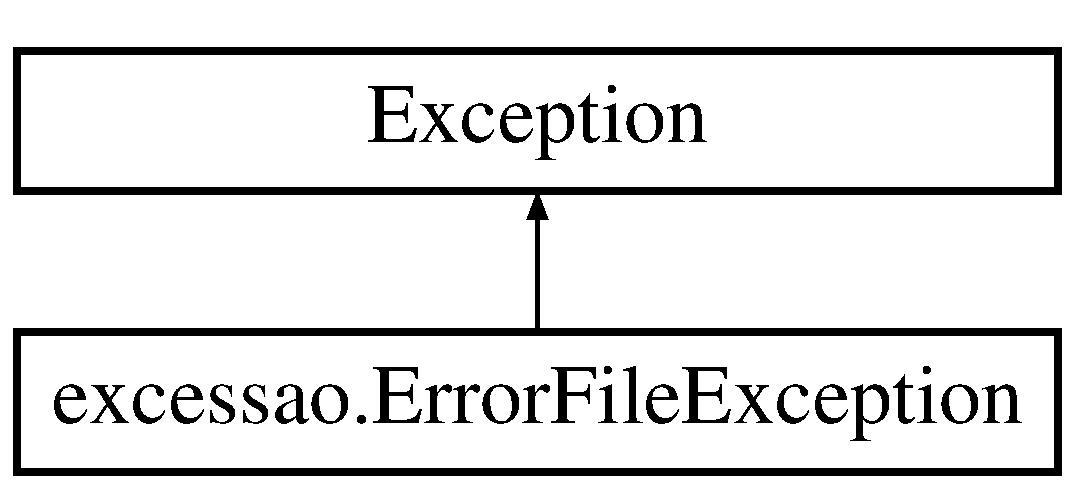
\includegraphics[height=2.000000cm]{classexcessao_1_1ErrorFileException}
\end{center}
\end{figure}
\subsection*{Public Member Functions}
\begin{DoxyCompactItemize}
\item 
String \hyperlink{classexcessao_1_1ErrorFileException_af764a39592ff12424d4dd76ef9c1fc30}{to\+String} ()
\item 
String \hyperlink{classexcessao_1_1ErrorFileException_a9503bc596c17f4a9bde0bb3fe7d12b0a}{get\+Message} ()
\end{DoxyCompactItemize}


\subsection{Detailed Description}


Definition at line 4 of file Error\+File\+Exception.\+java.



\subsection{Member Function Documentation}
\hypertarget{classexcessao_1_1ErrorFileException_a9503bc596c17f4a9bde0bb3fe7d12b0a}{}\label{classexcessao_1_1ErrorFileException_a9503bc596c17f4a9bde0bb3fe7d12b0a} 
\index{excessao\+::\+Error\+File\+Exception@{excessao\+::\+Error\+File\+Exception}!get\+Message@{get\+Message}}
\index{get\+Message@{get\+Message}!excessao\+::\+Error\+File\+Exception@{excessao\+::\+Error\+File\+Exception}}
\subsubsection{\texorpdfstring{get\+Message()}{getMessage()}}
{\footnotesize\ttfamily String excessao.\+Error\+File\+Exception.\+get\+Message (\begin{DoxyParamCaption}{ }\end{DoxyParamCaption})}



Definition at line 11 of file Error\+File\+Exception.\+java.

\hypertarget{classexcessao_1_1ErrorFileException_af764a39592ff12424d4dd76ef9c1fc30}{}\label{classexcessao_1_1ErrorFileException_af764a39592ff12424d4dd76ef9c1fc30} 
\index{excessao\+::\+Error\+File\+Exception@{excessao\+::\+Error\+File\+Exception}!to\+String@{to\+String}}
\index{to\+String@{to\+String}!excessao\+::\+Error\+File\+Exception@{excessao\+::\+Error\+File\+Exception}}
\subsubsection{\texorpdfstring{to\+String()}{toString()}}
{\footnotesize\ttfamily String excessao.\+Error\+File\+Exception.\+to\+String (\begin{DoxyParamCaption}{ }\end{DoxyParamCaption})}



Definition at line 6 of file Error\+File\+Exception.\+java.



The documentation for this class was generated from the following file\+:\begin{DoxyCompactItemize}
\item 
excessao/\hyperlink{ErrorFileException_8java}{Error\+File\+Exception.\+java}\end{DoxyCompactItemize}

\hypertarget{classDAO_1_1File}{}\section{D\+A\+O.\+File Class Reference}
\label{classDAO_1_1File}\index{D\+A\+O.\+File@{D\+A\+O.\+File}}
\subsection*{Static Public Member Functions}
\begin{DoxyCompactItemize}
\item 
static String \hyperlink{classDAO_1_1File_a348c16a4685741546b894803f95fc8b7}{read\+File} (String path)  throws Error\+File\+Exception 
\item 
static String \hyperlink{classDAO_1_1File_ae6b4d0d0dc80f0e783e78bee62c3f7fe}{read\+Prefixed\+File} (String path)  throws Error\+File\+Exception 
\item 
static void \hyperlink{classDAO_1_1File_aff9e42d1f5bc8fbf1e70426585c09240}{write\+File} (String path, String text)  throws I\+O\+Exception 
\item 
static java.\+io.\+File \mbox{[}$\,$\mbox{]} \hyperlink{classDAO_1_1File_abd456e59e6420b8bd4b534c5ffa33158}{list\+Files} ()
\end{DoxyCompactItemize}


\subsection{Detailed Description}
Intermedia as operações de leitura e escrita no disco.

\begin{DoxyAuthor}{Author}
Geovani Celebrim 
\end{DoxyAuthor}


Definition at line 18 of file File.\+java.



\subsection{Member Function Documentation}
\hypertarget{classDAO_1_1File_abd456e59e6420b8bd4b534c5ffa33158}{}\label{classDAO_1_1File_abd456e59e6420b8bd4b534c5ffa33158} 
\index{D\+A\+O\+::\+File@{D\+A\+O\+::\+File}!list\+Files@{list\+Files}}
\index{list\+Files@{list\+Files}!D\+A\+O\+::\+File@{D\+A\+O\+::\+File}}
\subsubsection{\texorpdfstring{list\+Files()}{listFiles()}}
{\footnotesize\ttfamily static java.\+io.\+File \mbox{[}$\,$\mbox{]} D\+A\+O.\+File.\+list\+Files (\begin{DoxyParamCaption}{ }\end{DoxyParamCaption})\hspace{0.3cm}{\ttfamily [static]}}

Lista os arquivos do diretório fixado em \hyperlink{enumDAO_1_1Authentication}{Authentication}.

\begin{DoxyReturn}{Returns}
\hyperlink{classDAO_1_1File}{File}\mbox{[}\mbox{]} que é um array de nomes de arquivos contidos no diretório fixado. 
\end{DoxyReturn}


Definition at line 113 of file File.\+java.



References D\+A\+O.\+Paths.\+D\+A\+T\+A\+\_\+\+T\+E\+XT, and D\+A\+O.\+Paths.\+F\+O\+L\+D\+ER.



Referenced by controlador.\+Simple\+Search.\+simple\+Search().

\hypertarget{classDAO_1_1File_a348c16a4685741546b894803f95fc8b7}{}\label{classDAO_1_1File_a348c16a4685741546b894803f95fc8b7} 
\index{D\+A\+O\+::\+File@{D\+A\+O\+::\+File}!read\+File@{read\+File}}
\index{read\+File@{read\+File}!D\+A\+O\+::\+File@{D\+A\+O\+::\+File}}
\subsubsection{\texorpdfstring{read\+File()}{readFile()}}
{\footnotesize\ttfamily static String D\+A\+O.\+File.\+read\+File (\begin{DoxyParamCaption}\item[{String}]{path }\end{DoxyParamCaption}) throws \hyperlink{classexcessao_1_1ErrorFileException}{Error\+File\+Exception}\hspace{0.3cm}{\ttfamily [static]}}

Lê o arquivo passado por parâmetro e retorna uma String com o seu conteúdo.


\begin{DoxyParams}{Parameters}
{\em path} & que é uma String o contendo caminho do arquivo. \\
\hline
\end{DoxyParams}
\begin{DoxyReturn}{Returns}
{\bfseries String} contendo as informações internas do arquivo. 
\end{DoxyReturn}

\begin{DoxyExceptions}{Exceptions}
{\em Error\+File\+Exception} & informando que não foi possível realizar a leitura do arquivo. \\
\hline
\end{DoxyExceptions}


Definition at line 30 of file File.\+java.



Referenced by D\+A\+O.\+Neo4j\+\_\+\+Rest.\+rest\+\_\+query().

\hypertarget{classDAO_1_1File_ae6b4d0d0dc80f0e783e78bee62c3f7fe}{}\label{classDAO_1_1File_ae6b4d0d0dc80f0e783e78bee62c3f7fe} 
\index{D\+A\+O\+::\+File@{D\+A\+O\+::\+File}!read\+Prefixed\+File@{read\+Prefixed\+File}}
\index{read\+Prefixed\+File@{read\+Prefixed\+File}!D\+A\+O\+::\+File@{D\+A\+O\+::\+File}}
\subsubsection{\texorpdfstring{read\+Prefixed\+File()}{readPrefixedFile()}}
{\footnotesize\ttfamily static String D\+A\+O.\+File.\+read\+Prefixed\+File (\begin{DoxyParamCaption}\item[{String}]{path }\end{DoxyParamCaption}) throws \hyperlink{classexcessao_1_1ErrorFileException}{Error\+File\+Exception}\hspace{0.3cm}{\ttfamily [static]}}

Lê o arquivo passado por parâmetro, que se localiza em um diretório prefixado em \hyperlink{enumDAO_1_1Authentication}{Authentication} e retorna uma String com o seu conteúdo.


\begin{DoxyParams}{Parameters}
{\em path} & que é uma String contendo o nome do arquivo. \\
\hline
\end{DoxyParams}
\begin{DoxyReturn}{Returns}
{\bfseries String} contendo as informações internas do arquivo. 
\end{DoxyReturn}

\begin{DoxyExceptions}{Exceptions}
{\em Error\+File\+Exception} & informando que não foi possível realizar a leitura do arquivo. \\
\hline
\end{DoxyExceptions}


Definition at line 63 of file File.\+java.



References D\+A\+O.\+Paths.\+D\+A\+T\+A\+\_\+\+T\+E\+XT.



Referenced by controlador.\+Semantics\+Search.\+document\+Search(), and controlador.\+servlets.\+Pagina\+Resultados.\+processar\+Requisicao().

\hypertarget{classDAO_1_1File_aff9e42d1f5bc8fbf1e70426585c09240}{}\label{classDAO_1_1File_aff9e42d1f5bc8fbf1e70426585c09240} 
\index{D\+A\+O\+::\+File@{D\+A\+O\+::\+File}!write\+File@{write\+File}}
\index{write\+File@{write\+File}!D\+A\+O\+::\+File@{D\+A\+O\+::\+File}}
\subsubsection{\texorpdfstring{write\+File()}{writeFile()}}
{\footnotesize\ttfamily static void D\+A\+O.\+File.\+write\+File (\begin{DoxyParamCaption}\item[{String}]{path,  }\item[{String}]{text }\end{DoxyParamCaption}) throws I\+O\+Exception\hspace{0.3cm}{\ttfamily [static]}}

Escreve no arquivo passado por parâmetro, o texto, também passado por parâmetro. Caso não seja possível realizar a escrita, é lançada uma excessão.


\begin{DoxyParams}{Parameters}
{\em path} & que é o caminho e nome do arquivo. \\
\hline
{\em text} & que é o texto a ser escrito no arquivo. \\
\hline
\end{DoxyParams}

\begin{DoxyExceptions}{Exceptions}
{\em I\+O\+Exception} & caso não seja possível a escrita. \\
\hline
\end{DoxyExceptions}


Definition at line 98 of file File.\+java.



Referenced by D\+A\+O.\+Neo4j\+\_\+\+Rest.\+rest\+\_\+query().



The documentation for this class was generated from the following file\+:\begin{DoxyCompactItemize}
\item 
D\+A\+O/\hyperlink{File_8java}{File.\+java}\end{DoxyCompactItemize}

\hypertarget{classentidade_1_1Graph}{}\section{entidade.\+Graph Class Reference}
\label{classentidade_1_1Graph}\index{entidade.\+Graph@{entidade.\+Graph}}
\subsection*{Public Member Functions}
\begin{DoxyCompactItemize}
\item 
\hyperlink{classentidade_1_1Graph_a8198c0f5c431837a3703d1473ab226ee}{Graph} ()
\item 
void \hyperlink{classentidade_1_1Graph_a95cb77104c1025c3628f614a299421ab}{adicionar\+Vertice} (\hyperlink{classentidade_1_1Vertex}{Vertex} vertice)
\item 
void \hyperlink{classentidade_1_1Graph_a284be62e0044149ea34122fabcdf1ace}{add\+Edge} (\hyperlink{classentidade_1_1Edge}{Edge} aresta)
\item 
Array\+List$<$ \hyperlink{classentidade_1_1Vertex}{Vertex} $>$ \hyperlink{classentidade_1_1Graph_a680550908cc41c83b901fb795cbbfd47}{get\+Vertices} ()
\item 
Array\+List$<$ \hyperlink{classentidade_1_1Edge}{Edge} $>$ \hyperlink{classentidade_1_1Graph_a36fc05f2c89421c63f9538bf280e54bb}{get\+Arestas} ()
\end{DoxyCompactItemize}


\subsection{Detailed Description}


Definition at line 5 of file Graph.\+java.



\subsection{Constructor \& Destructor Documentation}
\hypertarget{classentidade_1_1Graph_a8198c0f5c431837a3703d1473ab226ee}{}\label{classentidade_1_1Graph_a8198c0f5c431837a3703d1473ab226ee} 
\index{entidade\+::\+Graph@{entidade\+::\+Graph}!Graph@{Graph}}
\index{Graph@{Graph}!entidade\+::\+Graph@{entidade\+::\+Graph}}
\subsubsection{\texorpdfstring{Graph()}{Graph()}}
{\footnotesize\ttfamily entidade.\+Graph.\+Graph (\begin{DoxyParamCaption}{ }\end{DoxyParamCaption})}



Definition at line 9 of file Graph.\+java.



\subsection{Member Function Documentation}
\hypertarget{classentidade_1_1Graph_a284be62e0044149ea34122fabcdf1ace}{}\label{classentidade_1_1Graph_a284be62e0044149ea34122fabcdf1ace} 
\index{entidade\+::\+Graph@{entidade\+::\+Graph}!add\+Edge@{add\+Edge}}
\index{add\+Edge@{add\+Edge}!entidade\+::\+Graph@{entidade\+::\+Graph}}
\subsubsection{\texorpdfstring{add\+Edge()}{addEdge()}}
{\footnotesize\ttfamily void entidade.\+Graph.\+add\+Edge (\begin{DoxyParamCaption}\item[{\hyperlink{classentidade_1_1Edge}{Edge}}]{aresta }\end{DoxyParamCaption})}



Definition at line 18 of file Graph.\+java.



Referenced by D\+A\+O.\+Neo4j\+\_\+\+Rest.\+builder\+Graph().

\hypertarget{classentidade_1_1Graph_a95cb77104c1025c3628f614a299421ab}{}\label{classentidade_1_1Graph_a95cb77104c1025c3628f614a299421ab} 
\index{entidade\+::\+Graph@{entidade\+::\+Graph}!adicionar\+Vertice@{adicionar\+Vertice}}
\index{adicionar\+Vertice@{adicionar\+Vertice}!entidade\+::\+Graph@{entidade\+::\+Graph}}
\subsubsection{\texorpdfstring{adicionar\+Vertice()}{adicionarVertice()}}
{\footnotesize\ttfamily void entidade.\+Graph.\+adicionar\+Vertice (\begin{DoxyParamCaption}\item[{\hyperlink{classentidade_1_1Vertex}{Vertex}}]{vertice }\end{DoxyParamCaption})}



Definition at line 14 of file Graph.\+java.



Referenced by D\+A\+O.\+Neo4j\+\_\+\+Rest.\+builder\+Graph().

\hypertarget{classentidade_1_1Graph_a36fc05f2c89421c63f9538bf280e54bb}{}\label{classentidade_1_1Graph_a36fc05f2c89421c63f9538bf280e54bb} 
\index{entidade\+::\+Graph@{entidade\+::\+Graph}!get\+Arestas@{get\+Arestas}}
\index{get\+Arestas@{get\+Arestas}!entidade\+::\+Graph@{entidade\+::\+Graph}}
\subsubsection{\texorpdfstring{get\+Arestas()}{getArestas()}}
{\footnotesize\ttfamily Array\+List$<$\hyperlink{classentidade_1_1Edge}{Edge}$>$ entidade.\+Graph.\+get\+Arestas (\begin{DoxyParamCaption}{ }\end{DoxyParamCaption})}



Definition at line 26 of file Graph.\+java.

\hypertarget{classentidade_1_1Graph_a680550908cc41c83b901fb795cbbfd47}{}\label{classentidade_1_1Graph_a680550908cc41c83b901fb795cbbfd47} 
\index{entidade\+::\+Graph@{entidade\+::\+Graph}!get\+Vertices@{get\+Vertices}}
\index{get\+Vertices@{get\+Vertices}!entidade\+::\+Graph@{entidade\+::\+Graph}}
\subsubsection{\texorpdfstring{get\+Vertices()}{getVertices()}}
{\footnotesize\ttfamily Array\+List$<$\hyperlink{classentidade_1_1Vertex}{Vertex}$>$ entidade.\+Graph.\+get\+Vertices (\begin{DoxyParamCaption}{ }\end{DoxyParamCaption})}



Definition at line 22 of file Graph.\+java.



The documentation for this class was generated from the following file\+:\begin{DoxyCompactItemize}
\item 
entidade/\hyperlink{Graph_8java}{Graph.\+java}\end{DoxyCompactItemize}

\hypertarget{classDAO_1_1Neo4j}{}\section{D\+A\+O.\+Neo4j Class Reference}
\label{classDAO_1_1Neo4j}\index{D\+A\+O.\+Neo4j@{D\+A\+O.\+Neo4j}}
\subsection*{Public Member Functions}
\begin{DoxyCompactItemize}
\item 
\hyperlink{classDAO_1_1Neo4j_af58dea23a60d5a3d38de5846b4aa0d47}{Neo4j} ()
\item 
Session \hyperlink{classDAO_1_1Neo4j_adcb642f9deb65fb53f10dbc2b16efd95}{get\+Session} ()
\item 
void \hyperlink{classDAO_1_1Neo4j_acf7e0b06aef5d1280ebe29857b6edd1c}{disconnect} ()
\end{DoxyCompactItemize}
\subsection*{Private Attributes}
\begin{DoxyCompactItemize}
\item 
Driver \hyperlink{classDAO_1_1Neo4j_ae39f48e933894d2bc2c742a1e6f39fa7}{driver}
\item 
Session \hyperlink{classDAO_1_1Neo4j_a504ee636d54273588fb7dd480c7bb1ee}{session}
\end{DoxyCompactItemize}


\subsection{Detailed Description}
Responsável por realizar as conexções com o banco através do {\itshape bolt}.

\begin{DoxyAuthor}{Author}
Geovani Celebrim 
\end{DoxyAuthor}


Definition at line 14 of file Neo4j.\+java.



\subsection{Constructor \& Destructor Documentation}
\hypertarget{classDAO_1_1Neo4j_af58dea23a60d5a3d38de5846b4aa0d47}{}\label{classDAO_1_1Neo4j_af58dea23a60d5a3d38de5846b4aa0d47} 
\index{D\+A\+O\+::\+Neo4j@{D\+A\+O\+::\+Neo4j}!Neo4j@{Neo4j}}
\index{Neo4j@{Neo4j}!D\+A\+O\+::\+Neo4j@{D\+A\+O\+::\+Neo4j}}
\subsubsection{\texorpdfstring{Neo4j()}{Neo4j()}}
{\footnotesize\ttfamily D\+A\+O.\+Neo4j.\+Neo4j (\begin{DoxyParamCaption}{ }\end{DoxyParamCaption})}

O construtor inicializa uma conexão com o banco, para que seja realizada uma consulta. 

Definition at line 24 of file Neo4j.\+java.



References D\+A\+O.\+Authentication.\+P\+A\+S\+S\+W\+O\+RD, and D\+A\+O.\+Authentication.\+U\+S\+ER.



\subsection{Member Function Documentation}
\hypertarget{classDAO_1_1Neo4j_acf7e0b06aef5d1280ebe29857b6edd1c}{}\label{classDAO_1_1Neo4j_acf7e0b06aef5d1280ebe29857b6edd1c} 
\index{D\+A\+O\+::\+Neo4j@{D\+A\+O\+::\+Neo4j}!disconnect@{disconnect}}
\index{disconnect@{disconnect}!D\+A\+O\+::\+Neo4j@{D\+A\+O\+::\+Neo4j}}
\subsubsection{\texorpdfstring{disconnect()}{disconnect()}}
{\footnotesize\ttfamily void D\+A\+O.\+Neo4j.\+disconnect (\begin{DoxyParamCaption}{ }\end{DoxyParamCaption})}

Finaliza a conexção com o banco. 

Definition at line 43 of file Neo4j.\+java.



Referenced by controlador.\+Semantics\+Search.\+cypher\+Search\+Bolt(), controlador.\+Simple\+Search.\+search\+Author(), util.\+Documents\+Data.\+search\+Author\+And\+Source(), and controlador.\+Simple\+Search.\+search\+Source().

\hypertarget{classDAO_1_1Neo4j_adcb642f9deb65fb53f10dbc2b16efd95}{}\label{classDAO_1_1Neo4j_adcb642f9deb65fb53f10dbc2b16efd95} 
\index{D\+A\+O\+::\+Neo4j@{D\+A\+O\+::\+Neo4j}!get\+Session@{get\+Session}}
\index{get\+Session@{get\+Session}!D\+A\+O\+::\+Neo4j@{D\+A\+O\+::\+Neo4j}}
\subsubsection{\texorpdfstring{get\+Session()}{getSession()}}
{\footnotesize\ttfamily Session D\+A\+O.\+Neo4j.\+get\+Session (\begin{DoxyParamCaption}{ }\end{DoxyParamCaption})}

Obtém a instância da sessão atual do banco.

\begin{DoxyReturn}{Returns}
{\bfseries Session.} 
\end{DoxyReturn}


Definition at line 36 of file Neo4j.\+java.



References D\+A\+O.\+Neo4j.\+session.



Referenced by controlador.\+Semantics\+Search.\+cypher\+Search\+Bolt(), controlador.\+Simple\+Search.\+search\+Author(), util.\+Documents\+Data.\+search\+Author\+And\+Source(), and controlador.\+Simple\+Search.\+search\+Source().



\subsection{Member Data Documentation}
\hypertarget{classDAO_1_1Neo4j_ae39f48e933894d2bc2c742a1e6f39fa7}{}\label{classDAO_1_1Neo4j_ae39f48e933894d2bc2c742a1e6f39fa7} 
\index{D\+A\+O\+::\+Neo4j@{D\+A\+O\+::\+Neo4j}!driver@{driver}}
\index{driver@{driver}!D\+A\+O\+::\+Neo4j@{D\+A\+O\+::\+Neo4j}}
\subsubsection{\texorpdfstring{driver}{driver}}
{\footnotesize\ttfamily Driver D\+A\+O.\+Neo4j.\+driver\hspace{0.3cm}{\ttfamily [private]}}



Definition at line 16 of file Neo4j.\+java.

\hypertarget{classDAO_1_1Neo4j_a504ee636d54273588fb7dd480c7bb1ee}{}\label{classDAO_1_1Neo4j_a504ee636d54273588fb7dd480c7bb1ee} 
\index{D\+A\+O\+::\+Neo4j@{D\+A\+O\+::\+Neo4j}!session@{session}}
\index{session@{session}!D\+A\+O\+::\+Neo4j@{D\+A\+O\+::\+Neo4j}}
\subsubsection{\texorpdfstring{session}{session}}
{\footnotesize\ttfamily Session D\+A\+O.\+Neo4j.\+session\hspace{0.3cm}{\ttfamily [private]}}



Definition at line 18 of file Neo4j.\+java.



Referenced by D\+A\+O.\+Neo4j.\+get\+Session().



The documentation for this class was generated from the following file\+:\begin{DoxyCompactItemize}
\item 
D\+A\+O/\hyperlink{Neo4j_8java}{Neo4j.\+java}\end{DoxyCompactItemize}

\hypertarget{classDAO_1_1Neo4j__Rest}{}\section{D\+A\+O.\+Neo4j\+\_\+\+Rest Class Reference}
\label{classDAO_1_1Neo4j__Rest}\index{D\+A\+O.\+Neo4j\+\_\+\+Rest@{D\+A\+O.\+Neo4j\+\_\+\+Rest}}
\subsection*{Static Public Member Functions}
\begin{DoxyCompactItemize}
\item 
static \hyperlink{classentidade_1_1Graph}{Graph} \hyperlink{classDAO_1_1Neo4j__Rest_ad77ecb3b275019e3186dbdd34dcedc6c}{get\+Graph} (String query)  throws Error\+File\+Exception, I\+O\+Exception 
\end{DoxyCompactItemize}
\subsection*{Static Private Member Functions}
\begin{DoxyCompactItemize}
\item 
static String \hyperlink{classDAO_1_1Neo4j__Rest_a6a3baef27da288379f39b90c7ca8b0a7}{rest\+\_\+query} (String query)  throws Error\+File\+Exception, 			\+I\+O\+Exception 
\item 
static \hyperlink{classentidade_1_1Graph}{Graph} \hyperlink{classDAO_1_1Neo4j__Rest_ac62f85a4a1155d1e2fa59d463530b722}{builder\+Graph} (String response)
\end{DoxyCompactItemize}


\subsection{Detailed Description}
Responsável por realizar as conexções com o banco usando {\itshape R\+E\+ST}.

\begin{DoxyAuthor}{Author}
Geovani Celebrim 
\end{DoxyAuthor}


Definition at line 16 of file Neo4j\+\_\+\+Rest.\+java.



\subsection{Member Function Documentation}
\hypertarget{classDAO_1_1Neo4j__Rest_ac62f85a4a1155d1e2fa59d463530b722}{}\label{classDAO_1_1Neo4j__Rest_ac62f85a4a1155d1e2fa59d463530b722} 
\index{D\+A\+O\+::\+Neo4j\+\_\+\+Rest@{D\+A\+O\+::\+Neo4j\+\_\+\+Rest}!builder\+Graph@{builder\+Graph}}
\index{builder\+Graph@{builder\+Graph}!D\+A\+O\+::\+Neo4j\+\_\+\+Rest@{D\+A\+O\+::\+Neo4j\+\_\+\+Rest}}
\subsubsection{\texorpdfstring{builder\+Graph()}{builderGraph()}}
{\footnotesize\ttfamily static \hyperlink{classentidade_1_1Graph}{Graph} D\+A\+O.\+Neo4j\+\_\+\+Rest.\+builder\+Graph (\begin{DoxyParamCaption}\item[{String}]{response }\end{DoxyParamCaption})\hspace{0.3cm}{\ttfamily [static]}, {\ttfamily [private]}}

Constroi um grafo com o {\itshape J\+S\+ON} retornado do banco. 
\begin{DoxyParams}{Parameters}
{\em response} & que é o que o banco retorna através do método rest\+\_\+query da classe \hyperlink{classDAO_1_1Neo4j__Rest}{Neo4j\+\_\+\+Rest}. \\
\hline
\end{DoxyParams}
\begin{DoxyReturn}{Returns}
{\bfseries Graph} construido a partir do {\bfseries response}. 
\end{DoxyReturn}


Definition at line 54 of file Neo4j\+\_\+\+Rest.\+java.



References entidade.\+Graph.\+add\+Edge(), and entidade.\+Graph.\+adicionar\+Vertice().



Referenced by D\+A\+O.\+Neo4j\+\_\+\+Rest.\+get\+Graph().

\hypertarget{classDAO_1_1Neo4j__Rest_ad77ecb3b275019e3186dbdd34dcedc6c}{}\label{classDAO_1_1Neo4j__Rest_ad77ecb3b275019e3186dbdd34dcedc6c} 
\index{D\+A\+O\+::\+Neo4j\+\_\+\+Rest@{D\+A\+O\+::\+Neo4j\+\_\+\+Rest}!get\+Graph@{get\+Graph}}
\index{get\+Graph@{get\+Graph}!D\+A\+O\+::\+Neo4j\+\_\+\+Rest@{D\+A\+O\+::\+Neo4j\+\_\+\+Rest}}
\subsubsection{\texorpdfstring{get\+Graph()}{getGraph()}}
{\footnotesize\ttfamily static \hyperlink{classentidade_1_1Graph}{Graph} D\+A\+O.\+Neo4j\+\_\+\+Rest.\+get\+Graph (\begin{DoxyParamCaption}\item[{String}]{query }\end{DoxyParamCaption}) throws \hyperlink{classexcessao_1_1ErrorFileException}{Error\+File\+Exception}, I\+O\+Exception\hspace{0.3cm}{\ttfamily [static]}}

Retorna um grafo, dada uma query em Cypher. 
\begin{DoxyParams}{Parameters}
{\em query} & String no formato Cypher. \\
\hline
\end{DoxyParams}
\begin{DoxyReturn}{Returns}
{\bfseries Graph}. 
\end{DoxyReturn}

\begin{DoxyExceptions}{Exceptions}
{\em Error\+File\+Exception} & caso ocorra erro nos métodos dependentes. \\
\hline
{\em I\+O\+Exception} & caso ocorra erro nos métodos dependentes. \\
\hline
\end{DoxyExceptions}


Definition at line 86 of file Neo4j\+\_\+\+Rest.\+java.



References D\+A\+O.\+Neo4j\+\_\+\+Rest.\+builder\+Graph(), and D\+A\+O.\+Neo4j\+\_\+\+Rest.\+rest\+\_\+query().



Referenced by controlador.\+Semantics\+Search.\+busca\+Cypher\+Rest().

\hypertarget{classDAO_1_1Neo4j__Rest_a6a3baef27da288379f39b90c7ca8b0a7}{}\label{classDAO_1_1Neo4j__Rest_a6a3baef27da288379f39b90c7ca8b0a7} 
\index{D\+A\+O\+::\+Neo4j\+\_\+\+Rest@{D\+A\+O\+::\+Neo4j\+\_\+\+Rest}!rest\+\_\+query@{rest\+\_\+query}}
\index{rest\+\_\+query@{rest\+\_\+query}!D\+A\+O\+::\+Neo4j\+\_\+\+Rest@{D\+A\+O\+::\+Neo4j\+\_\+\+Rest}}
\subsubsection{\texorpdfstring{rest\+\_\+query()}{rest\_query()}}
{\footnotesize\ttfamily static String D\+A\+O.\+Neo4j\+\_\+\+Rest.\+rest\+\_\+query (\begin{DoxyParamCaption}\item[{String}]{query }\end{DoxyParamCaption}) throws \hyperlink{classexcessao_1_1ErrorFileException}{Error\+File\+Exception}, 			I\+O\+Exception\hspace{0.3cm}{\ttfamily [static]}, {\ttfamily [private]}}

Sobrescreve um template em Python e realiza uma conexão com o banco para obter o {\itshape J\+S\+ON.} 
\begin{DoxyParams}{Parameters}
{\em query} & que é a consulta em Cypher a ser realizada. \\
\hline
\end{DoxyParams}
\begin{DoxyReturn}{Returns}
{\bfseries String} com o {\itshape J\+S\+ON} que representa um grafo. 
\end{DoxyReturn}

\begin{DoxyExceptions}{Exceptions}
{\em Error\+File\+Exception} & caso ocorra algum erro na sobrescrita. \\
\hline
{\em I\+O\+Exception} & caso ocorra algum erro na sobrescrita. \\
\hline
\end{DoxyExceptions}


Definition at line 24 of file Neo4j\+\_\+\+Rest.\+java.



References util.\+Sys.\+command(), D\+A\+O.\+Authentication.\+P\+A\+S\+S\+W\+O\+RD, D\+A\+O.\+File.\+read\+File(), D\+A\+O.\+Paths.\+R\+E\+ST, D\+A\+O.\+Authentication.\+U\+S\+ER, and D\+A\+O.\+File.\+write\+File().



Referenced by D\+A\+O.\+Neo4j\+\_\+\+Rest.\+get\+Graph().



The documentation for this class was generated from the following file\+:\begin{DoxyCompactItemize}
\item 
D\+A\+O/\hyperlink{Neo4j__Rest_8java}{Neo4j\+\_\+\+Rest.\+java}\end{DoxyCompactItemize}

\hypertarget{classcontrolador_1_1servlets_1_1PaginaPrincipal}{}\section{controlador.\+servlets.\+Pagina\+Principal Class Reference}
\label{classcontrolador_1_1servlets_1_1PaginaPrincipal}\index{controlador.\+servlets.\+Pagina\+Principal@{controlador.\+servlets.\+Pagina\+Principal}}
Inheritance diagram for controlador.\+servlets.\+Pagina\+Principal\+:\begin{figure}[H]
\begin{center}
\leavevmode
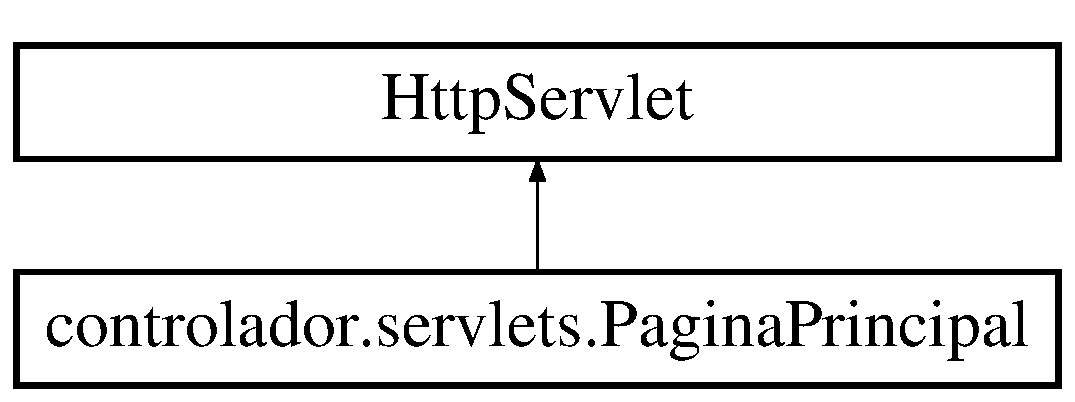
\includegraphics[height=2.000000cm]{classcontrolador_1_1servlets_1_1PaginaPrincipal}
\end{center}
\end{figure}
\subsection*{Public Member Functions}
\begin{DoxyCompactItemize}
\item 
\hyperlink{classcontrolador_1_1servlets_1_1PaginaPrincipal_a81b4ce3852074660b6c49ad8f9381db2}{Pagina\+Principal} ()
\end{DoxyCompactItemize}
\subsection*{Protected Member Functions}
\begin{DoxyCompactItemize}
\item 
void \hyperlink{classcontrolador_1_1servlets_1_1PaginaPrincipal_a1ebdc5a022ce170f3648fe141f9e1480}{do\+Get} (Http\+Servlet\+Request request, Http\+Servlet\+Response response)  throws Servlet\+Exception, I\+O\+Exception 
\item 
void \hyperlink{classcontrolador_1_1servlets_1_1PaginaPrincipal_ae33ae6fe9a5e9b39a5d9d58041b8b3ad}{do\+Post} (Http\+Servlet\+Request request, Http\+Servlet\+Response response)  throws Servlet\+Exception, I\+O\+Exception 
\end{DoxyCompactItemize}
\subsection*{Private Member Functions}
\begin{DoxyCompactItemize}
\item 
void \hyperlink{classcontrolador_1_1servlets_1_1PaginaPrincipal_a0a1fdddaf14f14c6454d400fb4cdc6f2}{processar\+Requisicao} (Http\+Servlet\+Request request, Http\+Servlet\+Response response)  throws Servlet\+Exception 
\item 
void \hyperlink{classcontrolador_1_1servlets_1_1PaginaPrincipal_a877a4f05faf8f1932e20cece0f7d39b7}{ir\+Para\+Resultados\+Semanticos} (Http\+Servlet\+Request request, Http\+Servlet\+Response response)
\item 
void \hyperlink{classcontrolador_1_1servlets_1_1PaginaPrincipal_a0aad40bb7b533fd6686c38b99b6aded8}{ir\+Para\+Resultados\+Simples} (Http\+Servlet\+Request request, Http\+Servlet\+Response response)
\end{DoxyCompactItemize}
\subsection*{Static Private Attributes}
\begin{DoxyCompactItemize}
\item 
static final long \hyperlink{classcontrolador_1_1servlets_1_1PaginaPrincipal_a49c31fd4aa9ba9711cd0e712eb5d805d}{serial\+Version\+U\+ID} = 1L
\end{DoxyCompactItemize}


\subsection{Detailed Description}


Definition at line 21 of file Pagina\+Principal.\+java.



\subsection{Constructor \& Destructor Documentation}
\hypertarget{classcontrolador_1_1servlets_1_1PaginaPrincipal_a81b4ce3852074660b6c49ad8f9381db2}{}\label{classcontrolador_1_1servlets_1_1PaginaPrincipal_a81b4ce3852074660b6c49ad8f9381db2} 
\index{controlador\+::servlets\+::\+Pagina\+Principal@{controlador\+::servlets\+::\+Pagina\+Principal}!Pagina\+Principal@{Pagina\+Principal}}
\index{Pagina\+Principal@{Pagina\+Principal}!controlador\+::servlets\+::\+Pagina\+Principal@{controlador\+::servlets\+::\+Pagina\+Principal}}
\subsubsection{\texorpdfstring{Pagina\+Principal()}{PaginaPrincipal()}}
{\footnotesize\ttfamily controlador.\+servlets.\+Pagina\+Principal.\+Pagina\+Principal (\begin{DoxyParamCaption}{ }\end{DoxyParamCaption})}



Definition at line 24 of file Pagina\+Principal.\+java.



\subsection{Member Function Documentation}
\hypertarget{classcontrolador_1_1servlets_1_1PaginaPrincipal_a1ebdc5a022ce170f3648fe141f9e1480}{}\label{classcontrolador_1_1servlets_1_1PaginaPrincipal_a1ebdc5a022ce170f3648fe141f9e1480} 
\index{controlador\+::servlets\+::\+Pagina\+Principal@{controlador\+::servlets\+::\+Pagina\+Principal}!do\+Get@{do\+Get}}
\index{do\+Get@{do\+Get}!controlador\+::servlets\+::\+Pagina\+Principal@{controlador\+::servlets\+::\+Pagina\+Principal}}
\subsubsection{\texorpdfstring{do\+Get()}{doGet()}}
{\footnotesize\ttfamily void controlador.\+servlets.\+Pagina\+Principal.\+do\+Get (\begin{DoxyParamCaption}\item[{Http\+Servlet\+Request}]{request,  }\item[{Http\+Servlet\+Response}]{response }\end{DoxyParamCaption}) throws Servlet\+Exception, I\+O\+Exception\hspace{0.3cm}{\ttfamily [protected]}}



Definition at line 132 of file Pagina\+Principal.\+java.

\hypertarget{classcontrolador_1_1servlets_1_1PaginaPrincipal_ae33ae6fe9a5e9b39a5d9d58041b8b3ad}{}\label{classcontrolador_1_1servlets_1_1PaginaPrincipal_ae33ae6fe9a5e9b39a5d9d58041b8b3ad} 
\index{controlador\+::servlets\+::\+Pagina\+Principal@{controlador\+::servlets\+::\+Pagina\+Principal}!do\+Post@{do\+Post}}
\index{do\+Post@{do\+Post}!controlador\+::servlets\+::\+Pagina\+Principal@{controlador\+::servlets\+::\+Pagina\+Principal}}
\subsubsection{\texorpdfstring{do\+Post()}{doPost()}}
{\footnotesize\ttfamily void controlador.\+servlets.\+Pagina\+Principal.\+do\+Post (\begin{DoxyParamCaption}\item[{Http\+Servlet\+Request}]{request,  }\item[{Http\+Servlet\+Response}]{response }\end{DoxyParamCaption}) throws Servlet\+Exception, I\+O\+Exception\hspace{0.3cm}{\ttfamily [protected]}}



Definition at line 138 of file Pagina\+Principal.\+java.

\hypertarget{classcontrolador_1_1servlets_1_1PaginaPrincipal_a877a4f05faf8f1932e20cece0f7d39b7}{}\label{classcontrolador_1_1servlets_1_1PaginaPrincipal_a877a4f05faf8f1932e20cece0f7d39b7} 
\index{controlador\+::servlets\+::\+Pagina\+Principal@{controlador\+::servlets\+::\+Pagina\+Principal}!ir\+Para\+Resultados\+Semanticos@{ir\+Para\+Resultados\+Semanticos}}
\index{ir\+Para\+Resultados\+Semanticos@{ir\+Para\+Resultados\+Semanticos}!controlador\+::servlets\+::\+Pagina\+Principal@{controlador\+::servlets\+::\+Pagina\+Principal}}
\subsubsection{\texorpdfstring{ir\+Para\+Resultados\+Semanticos()}{irParaResultadosSemanticos()}}
{\footnotesize\ttfamily void controlador.\+servlets.\+Pagina\+Principal.\+ir\+Para\+Resultados\+Semanticos (\begin{DoxyParamCaption}\item[{Http\+Servlet\+Request}]{request,  }\item[{Http\+Servlet\+Response}]{response }\end{DoxyParamCaption})\hspace{0.3cm}{\ttfamily [private]}}



Definition at line 104 of file Pagina\+Principal.\+java.

\hypertarget{classcontrolador_1_1servlets_1_1PaginaPrincipal_a0aad40bb7b533fd6686c38b99b6aded8}{}\label{classcontrolador_1_1servlets_1_1PaginaPrincipal_a0aad40bb7b533fd6686c38b99b6aded8} 
\index{controlador\+::servlets\+::\+Pagina\+Principal@{controlador\+::servlets\+::\+Pagina\+Principal}!ir\+Para\+Resultados\+Simples@{ir\+Para\+Resultados\+Simples}}
\index{ir\+Para\+Resultados\+Simples@{ir\+Para\+Resultados\+Simples}!controlador\+::servlets\+::\+Pagina\+Principal@{controlador\+::servlets\+::\+Pagina\+Principal}}
\subsubsection{\texorpdfstring{ir\+Para\+Resultados\+Simples()}{irParaResultadosSimples()}}
{\footnotesize\ttfamily void controlador.\+servlets.\+Pagina\+Principal.\+ir\+Para\+Resultados\+Simples (\begin{DoxyParamCaption}\item[{Http\+Servlet\+Request}]{request,  }\item[{Http\+Servlet\+Response}]{response }\end{DoxyParamCaption})\hspace{0.3cm}{\ttfamily [private]}}



Definition at line 118 of file Pagina\+Principal.\+java.

\hypertarget{classcontrolador_1_1servlets_1_1PaginaPrincipal_a0a1fdddaf14f14c6454d400fb4cdc6f2}{}\label{classcontrolador_1_1servlets_1_1PaginaPrincipal_a0a1fdddaf14f14c6454d400fb4cdc6f2} 
\index{controlador\+::servlets\+::\+Pagina\+Principal@{controlador\+::servlets\+::\+Pagina\+Principal}!processar\+Requisicao@{processar\+Requisicao}}
\index{processar\+Requisicao@{processar\+Requisicao}!controlador\+::servlets\+::\+Pagina\+Principal@{controlador\+::servlets\+::\+Pagina\+Principal}}
\subsubsection{\texorpdfstring{processar\+Requisicao()}{processarRequisicao()}}
{\footnotesize\ttfamily void controlador.\+servlets.\+Pagina\+Principal.\+processar\+Requisicao (\begin{DoxyParamCaption}\item[{Http\+Servlet\+Request}]{request,  }\item[{Http\+Servlet\+Response}]{response }\end{DoxyParamCaption}) throws Servlet\+Exception\hspace{0.3cm}{\ttfamily [private]}}



Definition at line 28 of file Pagina\+Principal.\+java.



References controlador.\+Semantics\+Search.\+busca\+Cypher\+Rest(), controlador.\+Semantics\+Search.\+cypher\+Search\+Bolt(), controlador.\+Semantics\+Search.\+document\+Search(), and controlador.\+Simple\+Search.\+simple\+Search().



\subsection{Member Data Documentation}
\hypertarget{classcontrolador_1_1servlets_1_1PaginaPrincipal_a49c31fd4aa9ba9711cd0e712eb5d805d}{}\label{classcontrolador_1_1servlets_1_1PaginaPrincipal_a49c31fd4aa9ba9711cd0e712eb5d805d} 
\index{controlador\+::servlets\+::\+Pagina\+Principal@{controlador\+::servlets\+::\+Pagina\+Principal}!serial\+Version\+U\+ID@{serial\+Version\+U\+ID}}
\index{serial\+Version\+U\+ID@{serial\+Version\+U\+ID}!controlador\+::servlets\+::\+Pagina\+Principal@{controlador\+::servlets\+::\+Pagina\+Principal}}
\subsubsection{\texorpdfstring{serial\+Version\+U\+ID}{serialVersionUID}}
{\footnotesize\ttfamily final long controlador.\+servlets.\+Pagina\+Principal.\+serial\+Version\+U\+ID = 1L\hspace{0.3cm}{\ttfamily [static]}, {\ttfamily [private]}}



Definition at line 22 of file Pagina\+Principal.\+java.



The documentation for this class was generated from the following file\+:\begin{DoxyCompactItemize}
\item 
controlador/servlets/\hyperlink{PaginaPrincipal_8java}{Pagina\+Principal.\+java}\end{DoxyCompactItemize}

\hypertarget{classcontrolador_1_1servlets_1_1PaginaResultados}{}\section{controlador.\+servlets.\+Pagina\+Resultados Class Reference}
\label{classcontrolador_1_1servlets_1_1PaginaResultados}\index{controlador.\+servlets.\+Pagina\+Resultados@{controlador.\+servlets.\+Pagina\+Resultados}}
Inheritance diagram for controlador.\+servlets.\+Pagina\+Resultados\+:\begin{figure}[H]
\begin{center}
\leavevmode
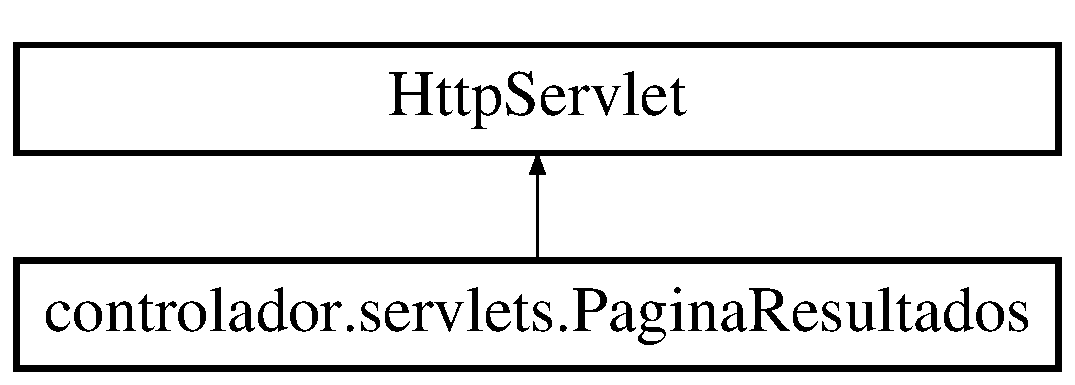
\includegraphics[height=2.000000cm]{classcontrolador_1_1servlets_1_1PaginaResultados}
\end{center}
\end{figure}
\subsection*{Public Member Functions}
\begin{DoxyCompactItemize}
\item 
\hyperlink{classcontrolador_1_1servlets_1_1PaginaResultados_add54c1c7fc8493235606b7675f67220b}{Pagina\+Resultados} ()
\end{DoxyCompactItemize}
\subsection*{Protected Member Functions}
\begin{DoxyCompactItemize}
\item 
void \hyperlink{classcontrolador_1_1servlets_1_1PaginaResultados_ab54c05fe6b07175f62c8902d3a58f885}{do\+Get} (Http\+Servlet\+Request request, Http\+Servlet\+Response response)  throws Servlet\+Exception, I\+O\+Exception 
\item 
void \hyperlink{classcontrolador_1_1servlets_1_1PaginaResultados_ac65f808df4a17b2e3f1cc36d8b5f69cd}{do\+Post} (Http\+Servlet\+Request request, Http\+Servlet\+Response response)  throws Servlet\+Exception, I\+O\+Exception 
\end{DoxyCompactItemize}
\subsection*{Private Member Functions}
\begin{DoxyCompactItemize}
\item 
void \hyperlink{classcontrolador_1_1servlets_1_1PaginaResultados_a4c45ab121c5b183b6a40aa3d0d3447de}{processar\+Requisicao} (Http\+Servlet\+Request request, Http\+Servlet\+Response response)  throws Servlet\+Exception 
\item 
void \hyperlink{classcontrolador_1_1servlets_1_1PaginaResultados_ab1ceb8a61e89cb50dc11aad9c79ac749}{ir\+Para\+Resultados\+Simples} (Http\+Servlet\+Request request, Http\+Servlet\+Response response)
\item 
void \hyperlink{classcontrolador_1_1servlets_1_1PaginaResultados_a900331c2d1545949444c5c88aeb7a03f}{ir\+Para\+Resultados\+Semanticos} (Http\+Servlet\+Request request, Http\+Servlet\+Response response)
\item 
void \hyperlink{classcontrolador_1_1servlets_1_1PaginaResultados_a4d8d584ec1bdfea0b521460a01f45e25}{ir\+Para\+Documento} (Http\+Servlet\+Request request, Http\+Servlet\+Response response)
\end{DoxyCompactItemize}
\subsection*{Static Private Attributes}
\begin{DoxyCompactItemize}
\item 
static final long \hyperlink{classcontrolador_1_1servlets_1_1PaginaResultados_a34b97ed1f44305439397ece4c6117929}{serial\+Version\+U\+ID} = 1L
\end{DoxyCompactItemize}


\subsection{Detailed Description}


Definition at line 22 of file Pagina\+Resultados.\+java.



\subsection{Constructor \& Destructor Documentation}
\hypertarget{classcontrolador_1_1servlets_1_1PaginaResultados_add54c1c7fc8493235606b7675f67220b}{}\label{classcontrolador_1_1servlets_1_1PaginaResultados_add54c1c7fc8493235606b7675f67220b} 
\index{controlador\+::servlets\+::\+Pagina\+Resultados@{controlador\+::servlets\+::\+Pagina\+Resultados}!Pagina\+Resultados@{Pagina\+Resultados}}
\index{Pagina\+Resultados@{Pagina\+Resultados}!controlador\+::servlets\+::\+Pagina\+Resultados@{controlador\+::servlets\+::\+Pagina\+Resultados}}
\subsubsection{\texorpdfstring{Pagina\+Resultados()}{PaginaResultados()}}
{\footnotesize\ttfamily controlador.\+servlets.\+Pagina\+Resultados.\+Pagina\+Resultados (\begin{DoxyParamCaption}{ }\end{DoxyParamCaption})}



Definition at line 25 of file Pagina\+Resultados.\+java.



\subsection{Member Function Documentation}
\hypertarget{classcontrolador_1_1servlets_1_1PaginaResultados_ab54c05fe6b07175f62c8902d3a58f885}{}\label{classcontrolador_1_1servlets_1_1PaginaResultados_ab54c05fe6b07175f62c8902d3a58f885} 
\index{controlador\+::servlets\+::\+Pagina\+Resultados@{controlador\+::servlets\+::\+Pagina\+Resultados}!do\+Get@{do\+Get}}
\index{do\+Get@{do\+Get}!controlador\+::servlets\+::\+Pagina\+Resultados@{controlador\+::servlets\+::\+Pagina\+Resultados}}
\subsubsection{\texorpdfstring{do\+Get()}{doGet()}}
{\footnotesize\ttfamily void controlador.\+servlets.\+Pagina\+Resultados.\+do\+Get (\begin{DoxyParamCaption}\item[{Http\+Servlet\+Request}]{request,  }\item[{Http\+Servlet\+Response}]{response }\end{DoxyParamCaption}) throws Servlet\+Exception, I\+O\+Exception\hspace{0.3cm}{\ttfamily [protected]}}



Definition at line 181 of file Pagina\+Resultados.\+java.

\hypertarget{classcontrolador_1_1servlets_1_1PaginaResultados_ac65f808df4a17b2e3f1cc36d8b5f69cd}{}\label{classcontrolador_1_1servlets_1_1PaginaResultados_ac65f808df4a17b2e3f1cc36d8b5f69cd} 
\index{controlador\+::servlets\+::\+Pagina\+Resultados@{controlador\+::servlets\+::\+Pagina\+Resultados}!do\+Post@{do\+Post}}
\index{do\+Post@{do\+Post}!controlador\+::servlets\+::\+Pagina\+Resultados@{controlador\+::servlets\+::\+Pagina\+Resultados}}
\subsubsection{\texorpdfstring{do\+Post()}{doPost()}}
{\footnotesize\ttfamily void controlador.\+servlets.\+Pagina\+Resultados.\+do\+Post (\begin{DoxyParamCaption}\item[{Http\+Servlet\+Request}]{request,  }\item[{Http\+Servlet\+Response}]{response }\end{DoxyParamCaption}) throws Servlet\+Exception, I\+O\+Exception\hspace{0.3cm}{\ttfamily [protected]}}



Definition at line 186 of file Pagina\+Resultados.\+java.

\hypertarget{classcontrolador_1_1servlets_1_1PaginaResultados_a4d8d584ec1bdfea0b521460a01f45e25}{}\label{classcontrolador_1_1servlets_1_1PaginaResultados_a4d8d584ec1bdfea0b521460a01f45e25} 
\index{controlador\+::servlets\+::\+Pagina\+Resultados@{controlador\+::servlets\+::\+Pagina\+Resultados}!ir\+Para\+Documento@{ir\+Para\+Documento}}
\index{ir\+Para\+Documento@{ir\+Para\+Documento}!controlador\+::servlets\+::\+Pagina\+Resultados@{controlador\+::servlets\+::\+Pagina\+Resultados}}
\subsubsection{\texorpdfstring{ir\+Para\+Documento()}{irParaDocumento()}}
{\footnotesize\ttfamily void controlador.\+servlets.\+Pagina\+Resultados.\+ir\+Para\+Documento (\begin{DoxyParamCaption}\item[{Http\+Servlet\+Request}]{request,  }\item[{Http\+Servlet\+Response}]{response }\end{DoxyParamCaption})\hspace{0.3cm}{\ttfamily [private]}}



Definition at line 167 of file Pagina\+Resultados.\+java.

\hypertarget{classcontrolador_1_1servlets_1_1PaginaResultados_a900331c2d1545949444c5c88aeb7a03f}{}\label{classcontrolador_1_1servlets_1_1PaginaResultados_a900331c2d1545949444c5c88aeb7a03f} 
\index{controlador\+::servlets\+::\+Pagina\+Resultados@{controlador\+::servlets\+::\+Pagina\+Resultados}!ir\+Para\+Resultados\+Semanticos@{ir\+Para\+Resultados\+Semanticos}}
\index{ir\+Para\+Resultados\+Semanticos@{ir\+Para\+Resultados\+Semanticos}!controlador\+::servlets\+::\+Pagina\+Resultados@{controlador\+::servlets\+::\+Pagina\+Resultados}}
\subsubsection{\texorpdfstring{ir\+Para\+Resultados\+Semanticos()}{irParaResultadosSemanticos()}}
{\footnotesize\ttfamily void controlador.\+servlets.\+Pagina\+Resultados.\+ir\+Para\+Resultados\+Semanticos (\begin{DoxyParamCaption}\item[{Http\+Servlet\+Request}]{request,  }\item[{Http\+Servlet\+Response}]{response }\end{DoxyParamCaption})\hspace{0.3cm}{\ttfamily [private]}}



Definition at line 153 of file Pagina\+Resultados.\+java.

\hypertarget{classcontrolador_1_1servlets_1_1PaginaResultados_ab1ceb8a61e89cb50dc11aad9c79ac749}{}\label{classcontrolador_1_1servlets_1_1PaginaResultados_ab1ceb8a61e89cb50dc11aad9c79ac749} 
\index{controlador\+::servlets\+::\+Pagina\+Resultados@{controlador\+::servlets\+::\+Pagina\+Resultados}!ir\+Para\+Resultados\+Simples@{ir\+Para\+Resultados\+Simples}}
\index{ir\+Para\+Resultados\+Simples@{ir\+Para\+Resultados\+Simples}!controlador\+::servlets\+::\+Pagina\+Resultados@{controlador\+::servlets\+::\+Pagina\+Resultados}}
\subsubsection{\texorpdfstring{ir\+Para\+Resultados\+Simples()}{irParaResultadosSimples()}}
{\footnotesize\ttfamily void controlador.\+servlets.\+Pagina\+Resultados.\+ir\+Para\+Resultados\+Simples (\begin{DoxyParamCaption}\item[{Http\+Servlet\+Request}]{request,  }\item[{Http\+Servlet\+Response}]{response }\end{DoxyParamCaption})\hspace{0.3cm}{\ttfamily [private]}}



Definition at line 139 of file Pagina\+Resultados.\+java.

\hypertarget{classcontrolador_1_1servlets_1_1PaginaResultados_a4c45ab121c5b183b6a40aa3d0d3447de}{}\label{classcontrolador_1_1servlets_1_1PaginaResultados_a4c45ab121c5b183b6a40aa3d0d3447de} 
\index{controlador\+::servlets\+::\+Pagina\+Resultados@{controlador\+::servlets\+::\+Pagina\+Resultados}!processar\+Requisicao@{processar\+Requisicao}}
\index{processar\+Requisicao@{processar\+Requisicao}!controlador\+::servlets\+::\+Pagina\+Resultados@{controlador\+::servlets\+::\+Pagina\+Resultados}}
\subsubsection{\texorpdfstring{processar\+Requisicao()}{processarRequisicao()}}
{\footnotesize\ttfamily void controlador.\+servlets.\+Pagina\+Resultados.\+processar\+Requisicao (\begin{DoxyParamCaption}\item[{Http\+Servlet\+Request}]{request,  }\item[{Http\+Servlet\+Response}]{response }\end{DoxyParamCaption}) throws Servlet\+Exception\hspace{0.3cm}{\ttfamily [private]}}



Definition at line 29 of file Pagina\+Resultados.\+java.



References controlador.\+Semantics\+Search.\+busca\+Cypher\+Rest(), controlador.\+Semantics\+Search.\+cypher\+Search\+Bolt(), controlador.\+Semantics\+Search.\+document\+Search(), D\+A\+O.\+File.\+read\+Prefixed\+File(), and controlador.\+Simple\+Search.\+simple\+Search().



\subsection{Member Data Documentation}
\hypertarget{classcontrolador_1_1servlets_1_1PaginaResultados_a34b97ed1f44305439397ece4c6117929}{}\label{classcontrolador_1_1servlets_1_1PaginaResultados_a34b97ed1f44305439397ece4c6117929} 
\index{controlador\+::servlets\+::\+Pagina\+Resultados@{controlador\+::servlets\+::\+Pagina\+Resultados}!serial\+Version\+U\+ID@{serial\+Version\+U\+ID}}
\index{serial\+Version\+U\+ID@{serial\+Version\+U\+ID}!controlador\+::servlets\+::\+Pagina\+Resultados@{controlador\+::servlets\+::\+Pagina\+Resultados}}
\subsubsection{\texorpdfstring{serial\+Version\+U\+ID}{serialVersionUID}}
{\footnotesize\ttfamily final long controlador.\+servlets.\+Pagina\+Resultados.\+serial\+Version\+U\+ID = 1L\hspace{0.3cm}{\ttfamily [static]}, {\ttfamily [private]}}



Definition at line 23 of file Pagina\+Resultados.\+java.



The documentation for this class was generated from the following file\+:\begin{DoxyCompactItemize}
\item 
controlador/servlets/\hyperlink{PaginaResultados_8java}{Pagina\+Resultados.\+java}\end{DoxyCompactItemize}

\hypertarget{enumDAO_1_1Paths}{}\section{D\+A\+O.\+Paths Enum Reference}
\label{enumDAO_1_1Paths}\index{D\+A\+O.\+Paths@{D\+A\+O.\+Paths}}
\subsection*{Public Member Functions}
\begin{DoxyCompactItemize}
\item 
String \hyperlink{enumDAO_1_1Paths_aec97ee6149db33c8d1880cf43ff3a77b}{to\+String} ()
\end{DoxyCompactItemize}
\subsection*{Public Attributes}
\begin{DoxyCompactItemize}
\item 
\hyperlink{enumDAO_1_1Paths_ab64a399f7d835455b9cf0b1207192eb0}{D\+A\+T\+A\+\_\+\+T\+E\+XT} =(\char`\"{}/home/geovani/cedim-\/data/\char`\"{})
\item 
\hyperlink{enumDAO_1_1Paths_a59211c627b8e37937625d10bcfab4899}{F\+O\+L\+D\+ER} =(\char`\"{}/C\+E\+D\+IM-\/II-\/G\+U\+E\+R\+RA\char`\"{})
\item 
\hyperlink{enumDAO_1_1Paths_a43cc47a733e9d706d1b299cb16a13f7a}{R\+E\+ST} =(\char`\"{}/home/geovani/git/tcc/Buscador\+Semantico/rest/\char`\"{})
\end{DoxyCompactItemize}
\subsection*{Private Member Functions}
\begin{DoxyCompactItemize}
\item 
\hyperlink{enumDAO_1_1Paths_a7986fd29f6dec9c0c8d6d28574b81b1c}{Paths} (final String \hyperlink{enumDAO_1_1Paths_aea7fb1a9db7ac0c55f6f7c9c81852d98}{text})
\end{DoxyCompactItemize}
\subsection*{Private Attributes}
\begin{DoxyCompactItemize}
\item 
final String \hyperlink{enumDAO_1_1Paths_aea7fb1a9db7ac0c55f6f7c9c81852d98}{text}
\end{DoxyCompactItemize}


\subsection{Detailed Description}
Esta classe tem como finalidade informar os diretórior de arquivos utilizados no sistema. O principal objetivo é centralizar as alterações, para que, caso necessário, essas informações sejam alteradas em apenas um local.

\begin{DoxyAuthor}{Author}
Geovani Celebrim 
\end{DoxyAuthor}


Definition at line 10 of file Paths.\+java.



\subsection{Constructor \& Destructor Documentation}
\hypertarget{enumDAO_1_1Paths_a7986fd29f6dec9c0c8d6d28574b81b1c}{}\label{enumDAO_1_1Paths_a7986fd29f6dec9c0c8d6d28574b81b1c} 
\index{D\+A\+O\+::\+Paths@{D\+A\+O\+::\+Paths}!Paths@{Paths}}
\index{Paths@{Paths}!D\+A\+O\+::\+Paths@{D\+A\+O\+::\+Paths}}
\subsubsection{\texorpdfstring{Paths()}{Paths()}}
{\footnotesize\ttfamily D\+A\+O.\+Paths.\+Paths (\begin{DoxyParamCaption}\item[{final String}]{text }\end{DoxyParamCaption})\hspace{0.3cm}{\ttfamily [private]}}



Definition at line 34 of file Paths.\+java.



\subsection{Member Function Documentation}
\hypertarget{enumDAO_1_1Paths_aec97ee6149db33c8d1880cf43ff3a77b}{}\label{enumDAO_1_1Paths_aec97ee6149db33c8d1880cf43ff3a77b} 
\index{D\+A\+O\+::\+Paths@{D\+A\+O\+::\+Paths}!to\+String@{to\+String}}
\index{to\+String@{to\+String}!D\+A\+O\+::\+Paths@{D\+A\+O\+::\+Paths}}
\subsubsection{\texorpdfstring{to\+String()}{toString()}}
{\footnotesize\ttfamily String D\+A\+O.\+Paths.\+to\+String (\begin{DoxyParamCaption}{ }\end{DoxyParamCaption})}

Pega o valor relacionado ao Enum em questão.

\begin{DoxyReturn}{Returns}
{\bfseries String} contendo o valor associado ao Enum.
\end{DoxyReturn}
\begin{DoxySeeAlso}{See also}
java.\+lang.\+Enum\+::to\+String() 

Enum 
\end{DoxySeeAlso}


Definition at line 47 of file Paths.\+java.



\subsection{Member Data Documentation}
\hypertarget{enumDAO_1_1Paths_ab64a399f7d835455b9cf0b1207192eb0}{}\label{enumDAO_1_1Paths_ab64a399f7d835455b9cf0b1207192eb0} 
\index{D\+A\+O\+::\+Paths@{D\+A\+O\+::\+Paths}!D\+A\+T\+A\+\_\+\+T\+E\+XT@{D\+A\+T\+A\+\_\+\+T\+E\+XT}}
\index{D\+A\+T\+A\+\_\+\+T\+E\+XT@{D\+A\+T\+A\+\_\+\+T\+E\+XT}!D\+A\+O\+::\+Paths@{D\+A\+O\+::\+Paths}}
\subsubsection{\texorpdfstring{D\+A\+T\+A\+\_\+\+T\+E\+XT}{DATA\_TEXT}}
{\footnotesize\ttfamily D\+A\+O.\+Paths.\+D\+A\+T\+A\+\_\+\+T\+E\+XT =(\char`\"{}/home/geovani/cedim-\/data/\char`\"{})}

Enum que representa o diretório de arquivos de texto retornados nas buscas. 

Definition at line 16 of file Paths.\+java.



Referenced by D\+A\+O.\+File.\+list\+Files(), and D\+A\+O.\+File.\+read\+Prefixed\+File().

\hypertarget{enumDAO_1_1Paths_a59211c627b8e37937625d10bcfab4899}{}\label{enumDAO_1_1Paths_a59211c627b8e37937625d10bcfab4899} 
\index{D\+A\+O\+::\+Paths@{D\+A\+O\+::\+Paths}!F\+O\+L\+D\+ER@{F\+O\+L\+D\+ER}}
\index{F\+O\+L\+D\+ER@{F\+O\+L\+D\+ER}!D\+A\+O\+::\+Paths@{D\+A\+O\+::\+Paths}}
\subsubsection{\texorpdfstring{F\+O\+L\+D\+ER}{FOLDER}}
{\footnotesize\ttfamily D\+A\+O.\+Paths.\+F\+O\+L\+D\+ER =(\char`\"{}/C\+E\+D\+IM-\/II-\/G\+U\+E\+R\+RA\char`\"{})}

Enum que representa a pasta dos dados utilizados no protótipo. 

Definition at line 23 of file Paths.\+java.



Referenced by D\+A\+O.\+File.\+list\+Files().

\hypertarget{enumDAO_1_1Paths_a43cc47a733e9d706d1b299cb16a13f7a}{}\label{enumDAO_1_1Paths_a43cc47a733e9d706d1b299cb16a13f7a} 
\index{D\+A\+O\+::\+Paths@{D\+A\+O\+::\+Paths}!R\+E\+ST@{R\+E\+ST}}
\index{R\+E\+ST@{R\+E\+ST}!D\+A\+O\+::\+Paths@{D\+A\+O\+::\+Paths}}
\subsubsection{\texorpdfstring{R\+E\+ST}{REST}}
{\footnotesize\ttfamily D\+A\+O.\+Paths.\+R\+E\+ST =(\char`\"{}/home/geovani/git/tcc/Buscador\+Semantico/rest/\char`\"{})}

Enum que representa o diretório do módulo em Python utilizado para conexão {\itshape R\+E\+ST} 

Definition at line 29 of file Paths.\+java.



Referenced by D\+A\+O.\+Neo4j\+\_\+\+Rest.\+rest\+\_\+query().

\hypertarget{enumDAO_1_1Paths_aea7fb1a9db7ac0c55f6f7c9c81852d98}{}\label{enumDAO_1_1Paths_aea7fb1a9db7ac0c55f6f7c9c81852d98} 
\index{D\+A\+O\+::\+Paths@{D\+A\+O\+::\+Paths}!text@{text}}
\index{text@{text}!D\+A\+O\+::\+Paths@{D\+A\+O\+::\+Paths}}
\subsubsection{\texorpdfstring{text}{text}}
{\footnotesize\ttfamily final String D\+A\+O.\+Paths.\+text\hspace{0.3cm}{\ttfamily [private]}}



Definition at line 32 of file Paths.\+java.



The documentation for this enum was generated from the following file\+:\begin{DoxyCompactItemize}
\item 
D\+A\+O/\hyperlink{Paths_8java}{Paths.\+java}\end{DoxyCompactItemize}

\hypertarget{classentidade_1_1Position}{}\section{entidade.\+Position Class Reference}
\label{classentidade_1_1Position}\index{entidade.\+Position@{entidade.\+Position}}
\subsection*{Public Member Functions}
\begin{DoxyCompactItemize}
\item 
\hyperlink{classentidade_1_1Position_a5c7ad4b5f26134b148dd56afa6bdcc60}{Position} (int inicio, int fim)
\item 
\hyperlink{classentidade_1_1Position_a2105dcad51d3f4924d5f0770958c529e}{Position} (String inicio, String fim)
\item 
int \hyperlink{classentidade_1_1Position_a1aa71cecbffd53debbe94973af2cca8c}{get\+Begin} ()
\item 
int \hyperlink{classentidade_1_1Position_aac6cfcd661388cf3faa47b6c80956e66}{get\+End} ()
\item 
String \hyperlink{classentidade_1_1Position_a65d216cd9c1de82bf23771f01a34c793}{to\+String} ()
\end{DoxyCompactItemize}


\subsection{Detailed Description}


Definition at line 3 of file Position.\+java.



\subsection{Constructor \& Destructor Documentation}
\hypertarget{classentidade_1_1Position_a5c7ad4b5f26134b148dd56afa6bdcc60}{}\label{classentidade_1_1Position_a5c7ad4b5f26134b148dd56afa6bdcc60} 
\index{entidade\+::\+Position@{entidade\+::\+Position}!Position@{Position}}
\index{Position@{Position}!entidade\+::\+Position@{entidade\+::\+Position}}
\subsubsection{\texorpdfstring{Position()}{Position()}\hspace{0.1cm}{\footnotesize\ttfamily [1/2]}}
{\footnotesize\ttfamily entidade.\+Position.\+Position (\begin{DoxyParamCaption}\item[{int}]{inicio,  }\item[{int}]{fim }\end{DoxyParamCaption})}



Definition at line 6 of file Position.\+java.

\hypertarget{classentidade_1_1Position_a2105dcad51d3f4924d5f0770958c529e}{}\label{classentidade_1_1Position_a2105dcad51d3f4924d5f0770958c529e} 
\index{entidade\+::\+Position@{entidade\+::\+Position}!Position@{Position}}
\index{Position@{Position}!entidade\+::\+Position@{entidade\+::\+Position}}
\subsubsection{\texorpdfstring{Position()}{Position()}\hspace{0.1cm}{\footnotesize\ttfamily [2/2]}}
{\footnotesize\ttfamily entidade.\+Position.\+Position (\begin{DoxyParamCaption}\item[{String}]{inicio,  }\item[{String}]{fim }\end{DoxyParamCaption})}



Definition at line 11 of file Position.\+java.



\subsection{Member Function Documentation}
\hypertarget{classentidade_1_1Position_a1aa71cecbffd53debbe94973af2cca8c}{}\label{classentidade_1_1Position_a1aa71cecbffd53debbe94973af2cca8c} 
\index{entidade\+::\+Position@{entidade\+::\+Position}!get\+Begin@{get\+Begin}}
\index{get\+Begin@{get\+Begin}!entidade\+::\+Position@{entidade\+::\+Position}}
\subsubsection{\texorpdfstring{get\+Begin()}{getBegin()}}
{\footnotesize\ttfamily int entidade.\+Position.\+get\+Begin (\begin{DoxyParamCaption}{ }\end{DoxyParamCaption})}



Definition at line 20 of file Position.\+java.

\hypertarget{classentidade_1_1Position_aac6cfcd661388cf3faa47b6c80956e66}{}\label{classentidade_1_1Position_aac6cfcd661388cf3faa47b6c80956e66} 
\index{entidade\+::\+Position@{entidade\+::\+Position}!get\+End@{get\+End}}
\index{get\+End@{get\+End}!entidade\+::\+Position@{entidade\+::\+Position}}
\subsubsection{\texorpdfstring{get\+End()}{getEnd()}}
{\footnotesize\ttfamily int entidade.\+Position.\+get\+End (\begin{DoxyParamCaption}{ }\end{DoxyParamCaption})}



Definition at line 24 of file Position.\+java.

\hypertarget{classentidade_1_1Position_a65d216cd9c1de82bf23771f01a34c793}{}\label{classentidade_1_1Position_a65d216cd9c1de82bf23771f01a34c793} 
\index{entidade\+::\+Position@{entidade\+::\+Position}!to\+String@{to\+String}}
\index{to\+String@{to\+String}!entidade\+::\+Position@{entidade\+::\+Position}}
\subsubsection{\texorpdfstring{to\+String()}{toString()}}
{\footnotesize\ttfamily String entidade.\+Position.\+to\+String (\begin{DoxyParamCaption}{ }\end{DoxyParamCaption})}



Definition at line 29 of file Position.\+java.



Referenced by entidade.\+resultados.\+Document\+Result.\+to\+String().



The documentation for this class was generated from the following file\+:\begin{DoxyCompactItemize}
\item 
entidade/\hyperlink{Position_8java}{Position.\+java}\end{DoxyCompactItemize}

\hypertarget{classexcessao_1_1QueryInvalidaException}{}\section{excessao.\+Query\+Invalida\+Exception Class Reference}
\label{classexcessao_1_1QueryInvalidaException}\index{excessao.\+Query\+Invalida\+Exception@{excessao.\+Query\+Invalida\+Exception}}
Inheritance diagram for excessao.\+Query\+Invalida\+Exception\+:\begin{figure}[H]
\begin{center}
\leavevmode
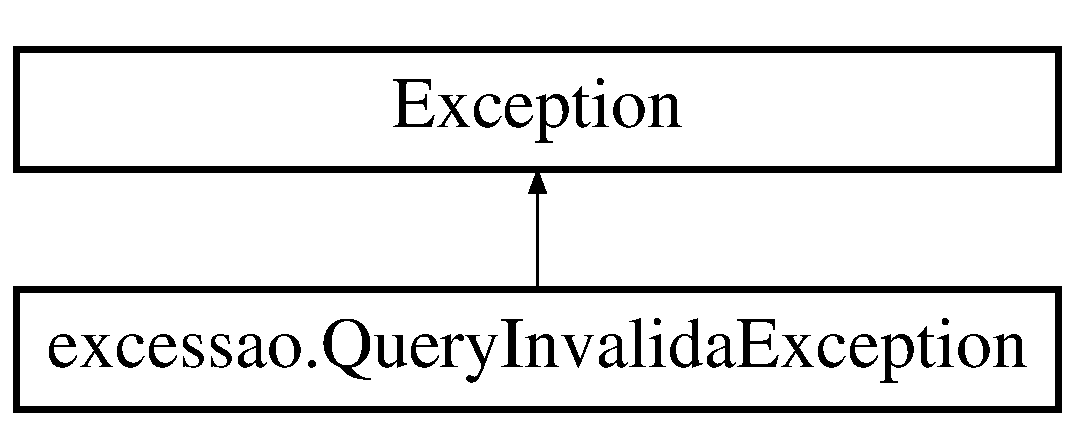
\includegraphics[height=2.000000cm]{classexcessao_1_1QueryInvalidaException}
\end{center}
\end{figure}
\subsection*{Public Member Functions}
\begin{DoxyCompactItemize}
\item 
String \hyperlink{classexcessao_1_1QueryInvalidaException_ac49499062d57f2eeefc351a1d14e5ce8}{to\+String} ()
\item 
String \hyperlink{classexcessao_1_1QueryInvalidaException_a22978d034834306fbaf113f7ff2f499f}{get\+Message} ()
\end{DoxyCompactItemize}


\subsection{Detailed Description}


Definition at line 4 of file Query\+Invalida\+Exception.\+java.



\subsection{Member Function Documentation}
\hypertarget{classexcessao_1_1QueryInvalidaException_a22978d034834306fbaf113f7ff2f499f}{}\label{classexcessao_1_1QueryInvalidaException_a22978d034834306fbaf113f7ff2f499f} 
\index{excessao\+::\+Query\+Invalida\+Exception@{excessao\+::\+Query\+Invalida\+Exception}!get\+Message@{get\+Message}}
\index{get\+Message@{get\+Message}!excessao\+::\+Query\+Invalida\+Exception@{excessao\+::\+Query\+Invalida\+Exception}}
\subsubsection{\texorpdfstring{get\+Message()}{getMessage()}}
{\footnotesize\ttfamily String excessao.\+Query\+Invalida\+Exception.\+get\+Message (\begin{DoxyParamCaption}{ }\end{DoxyParamCaption})}



Definition at line 11 of file Query\+Invalida\+Exception.\+java.

\hypertarget{classexcessao_1_1QueryInvalidaException_ac49499062d57f2eeefc351a1d14e5ce8}{}\label{classexcessao_1_1QueryInvalidaException_ac49499062d57f2eeefc351a1d14e5ce8} 
\index{excessao\+::\+Query\+Invalida\+Exception@{excessao\+::\+Query\+Invalida\+Exception}!to\+String@{to\+String}}
\index{to\+String@{to\+String}!excessao\+::\+Query\+Invalida\+Exception@{excessao\+::\+Query\+Invalida\+Exception}}
\subsubsection{\texorpdfstring{to\+String()}{toString()}}
{\footnotesize\ttfamily String excessao.\+Query\+Invalida\+Exception.\+to\+String (\begin{DoxyParamCaption}{ }\end{DoxyParamCaption})}



Definition at line 6 of file Query\+Invalida\+Exception.\+java.



The documentation for this class was generated from the following file\+:\begin{DoxyCompactItemize}
\item 
excessao/\hyperlink{QueryInvalidaException_8java}{Query\+Invalida\+Exception.\+java}\end{DoxyCompactItemize}

\hypertarget{classentidade_1_1resultados_1_1ResultadoGrafo}{}\section{entidade.\+resultados.\+Resultado\+Grafo Class Reference}
\label{classentidade_1_1resultados_1_1ResultadoGrafo}\index{entidade.\+resultados.\+Resultado\+Grafo@{entidade.\+resultados.\+Resultado\+Grafo}}


\subsection{Detailed Description}


Definition at line 3 of file Resultado\+Grafo.\+java.



The documentation for this class was generated from the following file\+:\begin{DoxyCompactItemize}
\item 
entidade/resultados/\hyperlink{ResultadoGrafo_8java}{Resultado\+Grafo.\+java}\end{DoxyCompactItemize}

\hypertarget{classcontrolador_1_1SemanticsSearch}{}\section{controlador.\+Semantics\+Search Class Reference}
\label{classcontrolador_1_1SemanticsSearch}\index{controlador.\+Semantics\+Search@{controlador.\+Semantics\+Search}}
\subsection*{Static Public Member Functions}
\begin{DoxyCompactItemize}
\item 
static Array\+List$<$ \hyperlink{classentidade_1_1resultados_1_1cypherResults}{cypher\+Results} $>$ \hyperlink{classcontrolador_1_1SemanticsSearch_a339848789ce165207406c6ee6f49c538}{cypher\+Search\+Bolt} (String cypher\+Query)  throws Exception 
\item 
static \hyperlink{classentidade_1_1Graph}{Graph} \hyperlink{classcontrolador_1_1SemanticsSearch_af6332056f2b69450b64220a5b11a69f4}{busca\+Cypher\+Rest} (String query)
\item 
static Array\+List$<$ \hyperlink{classentidade_1_1resultados_1_1DocumentResult}{Document\+Result} $>$ \hyperlink{classcontrolador_1_1SemanticsSearch_a0cd2e6b6e45fe9738ea91c606a48afef}{document\+Search} (String cypher\+Query)  throws Exception 
\end{DoxyCompactItemize}


\subsection{Detailed Description}
Controlador responsável por mediar as buscas semânticas no banco e no repositório de arquivos.

\begin{DoxyAuthor}{Author}
Geovani Celebrim 
\end{DoxyAuthor}


Definition at line 27 of file Semantics\+Search.\+java.



\subsection{Member Function Documentation}
\hypertarget{classcontrolador_1_1SemanticsSearch_af6332056f2b69450b64220a5b11a69f4}{}\label{classcontrolador_1_1SemanticsSearch_af6332056f2b69450b64220a5b11a69f4} 
\index{controlador\+::\+Semantics\+Search@{controlador\+::\+Semantics\+Search}!busca\+Cypher\+Rest@{busca\+Cypher\+Rest}}
\index{busca\+Cypher\+Rest@{busca\+Cypher\+Rest}!controlador\+::\+Semantics\+Search@{controlador\+::\+Semantics\+Search}}
\subsubsection{\texorpdfstring{busca\+Cypher\+Rest()}{buscaCypherRest()}}
{\footnotesize\ttfamily static \hyperlink{classentidade_1_1Graph}{Graph} controlador.\+Semantics\+Search.\+busca\+Cypher\+Rest (\begin{DoxyParamCaption}\item[{String}]{query }\end{DoxyParamCaption})\hspace{0.3cm}{\ttfamily [static]}}

Realiza uma busca no banco Neo4j, usando o módulo em Python, dada uma String no formato Cypher, e retorna um \hyperlink{}{Graph}.


\begin{DoxyParams}{Parameters}
{\em query} & String em formato Cypher. \\
\hline
\end{DoxyParams}
\begin{DoxyReturn}{Returns}
{\bfseries Graph} 
\end{DoxyReturn}


Definition at line 68 of file Semantics\+Search.\+java.



References D\+A\+O.\+Neo4j\+\_\+\+Rest.\+get\+Graph().



Referenced by controlador.\+servlets.\+Pagina\+Principal.\+processar\+Requisicao(), and controlador.\+servlets.\+Pagina\+Resultados.\+processar\+Requisicao().

\hypertarget{classcontrolador_1_1SemanticsSearch_a339848789ce165207406c6ee6f49c538}{}\label{classcontrolador_1_1SemanticsSearch_a339848789ce165207406c6ee6f49c538} 
\index{controlador\+::\+Semantics\+Search@{controlador\+::\+Semantics\+Search}!cypher\+Search\+Bolt@{cypher\+Search\+Bolt}}
\index{cypher\+Search\+Bolt@{cypher\+Search\+Bolt}!controlador\+::\+Semantics\+Search@{controlador\+::\+Semantics\+Search}}
\subsubsection{\texorpdfstring{cypher\+Search\+Bolt()}{cypherSearchBolt()}}
{\footnotesize\ttfamily static Array\+List$<$\hyperlink{classentidade_1_1resultados_1_1cypherResults}{cypher\+Results}$>$ controlador.\+Semantics\+Search.\+cypher\+Search\+Bolt (\begin{DoxyParamCaption}\item[{String}]{cypher\+Query }\end{DoxyParamCaption}) throws Exception\hspace{0.3cm}{\ttfamily [static]}}

Busca no banco Neo4j, dada uma String no formato Cypher, e retorna um \hyperlink{}{Array\+List} de \hyperlink{}{cypher\+Results}.


\begin{DoxyParams}{Parameters}
{\em cypher\+Query} & String no formato Cypher. \\
\hline
\end{DoxyParams}
\begin{DoxyReturn}{Returns}
{\bfseries Array\+List} de \hyperlink{}{cypher\+Results} contendo os resultados encontrados. 
\end{DoxyReturn}

\begin{DoxyExceptions}{Exceptions}
{\em Exception} & caso ocorra uma falha em algum passo da busca. \\
\hline
\end{DoxyExceptions}


Definition at line 41 of file Semantics\+Search.\+java.



References D\+A\+O.\+Neo4j.\+disconnect(), D\+A\+O.\+Neo4j.\+get\+Session(), and util.\+Data\+Processing.\+statement\+To\+Cypher().



Referenced by controlador.\+servlets.\+Pagina\+Principal.\+processar\+Requisicao(), and controlador.\+servlets.\+Pagina\+Resultados.\+processar\+Requisicao().

\hypertarget{classcontrolador_1_1SemanticsSearch_a0cd2e6b6e45fe9738ea91c606a48afef}{}\label{classcontrolador_1_1SemanticsSearch_a0cd2e6b6e45fe9738ea91c606a48afef} 
\index{controlador\+::\+Semantics\+Search@{controlador\+::\+Semantics\+Search}!document\+Search@{document\+Search}}
\index{document\+Search@{document\+Search}!controlador\+::\+Semantics\+Search@{controlador\+::\+Semantics\+Search}}
\subsubsection{\texorpdfstring{document\+Search()}{documentSearch()}}
{\footnotesize\ttfamily static Array\+List$<$\hyperlink{classentidade_1_1resultados_1_1DocumentResult}{Document\+Result}$>$ controlador.\+Semantics\+Search.\+document\+Search (\begin{DoxyParamCaption}\item[{String}]{cypher\+Query }\end{DoxyParamCaption}) throws Exception\hspace{0.3cm}{\ttfamily [static]}}

Realiza uma busca no banco Neo4j, dada uma String no formato Cypher, e retorna um \hyperlink{}{Array\+List} de \hyperlink{}{Document\+Result}. Essa busca cruza os dados do banco para obter o trecho onde a informação se encontra no documento.


\begin{DoxyParams}{Parameters}
{\em cypher\+Query} & String no formado Cypher. \\
\hline
\end{DoxyParams}
\begin{DoxyReturn}{Returns}
{\bfseries Array\+List} de \hyperlink{}{Document\+Result}. 
\end{DoxyReturn}

\begin{DoxyExceptions}{Exceptions}
{\em Exception} & caso ocorra algum erro na extração dos dados. \\
\hline
\end{DoxyExceptions}


Definition at line 104 of file Semantics\+Search.\+java.



References util.\+Documents\+Data.\+approaching\+Initial\+Index(), util.\+Data\+Processing.\+cross\+Data(), util.\+Documents\+Data.\+end\+Index(), entidade.\+resultados.\+Document\+Result.\+get\+Author(), entidade.\+resultados.\+Document\+Result.\+get\+Source(), D\+A\+O.\+File.\+read\+Prefixed\+File(), and util.\+Documents\+Data.\+search\+Author\+And\+Source().



Referenced by controlador.\+servlets.\+Pagina\+Principal.\+processar\+Requisicao(), and controlador.\+servlets.\+Pagina\+Resultados.\+processar\+Requisicao().



The documentation for this class was generated from the following file\+:\begin{DoxyCompactItemize}
\item 
controlador/\hyperlink{SemanticsSearch_8java}{Semantics\+Search.\+java}\end{DoxyCompactItemize}

\hypertarget{classentidade_1_1resultados_1_1SimpleResults}{}\section{entidade.\+resultados.\+Simple\+Results Class Reference}
\label{classentidade_1_1resultados_1_1SimpleResults}\index{entidade.\+resultados.\+Simple\+Results@{entidade.\+resultados.\+Simple\+Results}}
\subsection*{Public Member Functions}
\begin{DoxyCompactItemize}
\item 
\hyperlink{classentidade_1_1resultados_1_1SimpleResults_a36411d7a5b487a8cb8d49e5dc13cccc3}{Simple\+Results} (String \hyperlink{classentidade_1_1resultados_1_1SimpleResults_a9dec340294219ec16a2e2b42e68ba350}{nome\+Documento}, String \hyperlink{classentidade_1_1resultados_1_1SimpleResults_a94e8f77e73a35a3a544f30de1d4fa5b6}{trecho}, String \hyperlink{classentidade_1_1resultados_1_1SimpleResults_afc17e94212f3953a05f63f9de5d4c345}{autor}, String \hyperlink{classentidade_1_1resultados_1_1SimpleResults_a2442d65af6ba817cd26d5bd41ef8c65c}{fonte})
\item 
\hyperlink{classentidade_1_1resultados_1_1SimpleResults_a4096968b8553b2b79984846a6f51603d}{Simple\+Results} (String \hyperlink{classentidade_1_1resultados_1_1SimpleResults_a9dec340294219ec16a2e2b42e68ba350}{nome\+Documento})
\item 
\hyperlink{classentidade_1_1resultados_1_1SimpleResults_a812be57a6cbdee87ce754241eeae9bc0}{Simple\+Results} (String \hyperlink{classentidade_1_1resultados_1_1SimpleResults_afc17e94212f3953a05f63f9de5d4c345}{autor}, String \hyperlink{classentidade_1_1resultados_1_1SimpleResults_a2442d65af6ba817cd26d5bd41ef8c65c}{fonte})
\item 
String \hyperlink{classentidade_1_1resultados_1_1SimpleResults_a42841134beb2bdeada3038d4550bf177}{get\+Nome\+Documento} ()
\item 
String \hyperlink{classentidade_1_1resultados_1_1SimpleResults_ae3d772893f928871dd13263ba4453e11}{get\+Trecho} ()
\item 
String \hyperlink{classentidade_1_1resultados_1_1SimpleResults_a9d78a2cab567ec7193d5a0defdd8629c}{get\+Autor} ()
\item 
String \hyperlink{classentidade_1_1resultados_1_1SimpleResults_af74e679c1d8154f9c4fc247edda6abed}{get\+Fonte} ()
\item 
String \hyperlink{classentidade_1_1resultados_1_1SimpleResults_aed676e978f66a5e2fc11332124c9f91f}{to\+String} ()
\end{DoxyCompactItemize}
\subsection*{Private Attributes}
\begin{DoxyCompactItemize}
\item 
String \hyperlink{classentidade_1_1resultados_1_1SimpleResults_a9dec340294219ec16a2e2b42e68ba350}{nome\+Documento}
\item 
String \hyperlink{classentidade_1_1resultados_1_1SimpleResults_a94e8f77e73a35a3a544f30de1d4fa5b6}{trecho}
\item 
String \hyperlink{classentidade_1_1resultados_1_1SimpleResults_afc17e94212f3953a05f63f9de5d4c345}{autor}
\item 
String \hyperlink{classentidade_1_1resultados_1_1SimpleResults_a2442d65af6ba817cd26d5bd41ef8c65c}{fonte}
\end{DoxyCompactItemize}


\subsection{Detailed Description}


Definition at line 3 of file Simple\+Results.\+java.



\subsection{Constructor \& Destructor Documentation}
\hypertarget{classentidade_1_1resultados_1_1SimpleResults_a36411d7a5b487a8cb8d49e5dc13cccc3}{}\label{classentidade_1_1resultados_1_1SimpleResults_a36411d7a5b487a8cb8d49e5dc13cccc3} 
\index{entidade\+::resultados\+::\+Simple\+Results@{entidade\+::resultados\+::\+Simple\+Results}!Simple\+Results@{Simple\+Results}}
\index{Simple\+Results@{Simple\+Results}!entidade\+::resultados\+::\+Simple\+Results@{entidade\+::resultados\+::\+Simple\+Results}}
\subsubsection{\texorpdfstring{Simple\+Results()}{SimpleResults()}\hspace{0.1cm}{\footnotesize\ttfamily [1/3]}}
{\footnotesize\ttfamily entidade.\+resultados.\+Simple\+Results.\+Simple\+Results (\begin{DoxyParamCaption}\item[{String}]{nome\+Documento,  }\item[{String}]{trecho,  }\item[{String}]{autor,  }\item[{String}]{fonte }\end{DoxyParamCaption})}



Definition at line 9 of file Simple\+Results.\+java.



References entidade.\+resultados.\+Simple\+Results.\+autor, entidade.\+resultados.\+Simple\+Results.\+fonte, entidade.\+resultados.\+Simple\+Results.\+nome\+Documento, and entidade.\+resultados.\+Simple\+Results.\+trecho.

\hypertarget{classentidade_1_1resultados_1_1SimpleResults_a4096968b8553b2b79984846a6f51603d}{}\label{classentidade_1_1resultados_1_1SimpleResults_a4096968b8553b2b79984846a6f51603d} 
\index{entidade\+::resultados\+::\+Simple\+Results@{entidade\+::resultados\+::\+Simple\+Results}!Simple\+Results@{Simple\+Results}}
\index{Simple\+Results@{Simple\+Results}!entidade\+::resultados\+::\+Simple\+Results@{entidade\+::resultados\+::\+Simple\+Results}}
\subsubsection{\texorpdfstring{Simple\+Results()}{SimpleResults()}\hspace{0.1cm}{\footnotesize\ttfamily [2/3]}}
{\footnotesize\ttfamily entidade.\+resultados.\+Simple\+Results.\+Simple\+Results (\begin{DoxyParamCaption}\item[{String}]{nome\+Documento }\end{DoxyParamCaption})}



Definition at line 17 of file Simple\+Results.\+java.



References entidade.\+resultados.\+Simple\+Results.\+nome\+Documento.

\hypertarget{classentidade_1_1resultados_1_1SimpleResults_a812be57a6cbdee87ce754241eeae9bc0}{}\label{classentidade_1_1resultados_1_1SimpleResults_a812be57a6cbdee87ce754241eeae9bc0} 
\index{entidade\+::resultados\+::\+Simple\+Results@{entidade\+::resultados\+::\+Simple\+Results}!Simple\+Results@{Simple\+Results}}
\index{Simple\+Results@{Simple\+Results}!entidade\+::resultados\+::\+Simple\+Results@{entidade\+::resultados\+::\+Simple\+Results}}
\subsubsection{\texorpdfstring{Simple\+Results()}{SimpleResults()}\hspace{0.1cm}{\footnotesize\ttfamily [3/3]}}
{\footnotesize\ttfamily entidade.\+resultados.\+Simple\+Results.\+Simple\+Results (\begin{DoxyParamCaption}\item[{String}]{autor,  }\item[{String}]{fonte }\end{DoxyParamCaption})}



Definition at line 21 of file Simple\+Results.\+java.



References entidade.\+resultados.\+Simple\+Results.\+autor, and entidade.\+resultados.\+Simple\+Results.\+fonte.



\subsection{Member Function Documentation}
\hypertarget{classentidade_1_1resultados_1_1SimpleResults_a9d78a2cab567ec7193d5a0defdd8629c}{}\label{classentidade_1_1resultados_1_1SimpleResults_a9d78a2cab567ec7193d5a0defdd8629c} 
\index{entidade\+::resultados\+::\+Simple\+Results@{entidade\+::resultados\+::\+Simple\+Results}!get\+Autor@{get\+Autor}}
\index{get\+Autor@{get\+Autor}!entidade\+::resultados\+::\+Simple\+Results@{entidade\+::resultados\+::\+Simple\+Results}}
\subsubsection{\texorpdfstring{get\+Autor()}{getAutor()}}
{\footnotesize\ttfamily String entidade.\+resultados.\+Simple\+Results.\+get\+Autor (\begin{DoxyParamCaption}{ }\end{DoxyParamCaption})}



Definition at line 34 of file Simple\+Results.\+java.



References entidade.\+resultados.\+Simple\+Results.\+autor.

\hypertarget{classentidade_1_1resultados_1_1SimpleResults_af74e679c1d8154f9c4fc247edda6abed}{}\label{classentidade_1_1resultados_1_1SimpleResults_af74e679c1d8154f9c4fc247edda6abed} 
\index{entidade\+::resultados\+::\+Simple\+Results@{entidade\+::resultados\+::\+Simple\+Results}!get\+Fonte@{get\+Fonte}}
\index{get\+Fonte@{get\+Fonte}!entidade\+::resultados\+::\+Simple\+Results@{entidade\+::resultados\+::\+Simple\+Results}}
\subsubsection{\texorpdfstring{get\+Fonte()}{getFonte()}}
{\footnotesize\ttfamily String entidade.\+resultados.\+Simple\+Results.\+get\+Fonte (\begin{DoxyParamCaption}{ }\end{DoxyParamCaption})}



Definition at line 38 of file Simple\+Results.\+java.



References entidade.\+resultados.\+Simple\+Results.\+fonte.

\hypertarget{classentidade_1_1resultados_1_1SimpleResults_a42841134beb2bdeada3038d4550bf177}{}\label{classentidade_1_1resultados_1_1SimpleResults_a42841134beb2bdeada3038d4550bf177} 
\index{entidade\+::resultados\+::\+Simple\+Results@{entidade\+::resultados\+::\+Simple\+Results}!get\+Nome\+Documento@{get\+Nome\+Documento}}
\index{get\+Nome\+Documento@{get\+Nome\+Documento}!entidade\+::resultados\+::\+Simple\+Results@{entidade\+::resultados\+::\+Simple\+Results}}
\subsubsection{\texorpdfstring{get\+Nome\+Documento()}{getNomeDocumento()}}
{\footnotesize\ttfamily String entidade.\+resultados.\+Simple\+Results.\+get\+Nome\+Documento (\begin{DoxyParamCaption}{ }\end{DoxyParamCaption})}



Definition at line 26 of file Simple\+Results.\+java.



References entidade.\+resultados.\+Simple\+Results.\+nome\+Documento.

\hypertarget{classentidade_1_1resultados_1_1SimpleResults_ae3d772893f928871dd13263ba4453e11}{}\label{classentidade_1_1resultados_1_1SimpleResults_ae3d772893f928871dd13263ba4453e11} 
\index{entidade\+::resultados\+::\+Simple\+Results@{entidade\+::resultados\+::\+Simple\+Results}!get\+Trecho@{get\+Trecho}}
\index{get\+Trecho@{get\+Trecho}!entidade\+::resultados\+::\+Simple\+Results@{entidade\+::resultados\+::\+Simple\+Results}}
\subsubsection{\texorpdfstring{get\+Trecho()}{getTrecho()}}
{\footnotesize\ttfamily String entidade.\+resultados.\+Simple\+Results.\+get\+Trecho (\begin{DoxyParamCaption}{ }\end{DoxyParamCaption})}



Definition at line 30 of file Simple\+Results.\+java.



References entidade.\+resultados.\+Simple\+Results.\+trecho.

\hypertarget{classentidade_1_1resultados_1_1SimpleResults_aed676e978f66a5e2fc11332124c9f91f}{}\label{classentidade_1_1resultados_1_1SimpleResults_aed676e978f66a5e2fc11332124c9f91f} 
\index{entidade\+::resultados\+::\+Simple\+Results@{entidade\+::resultados\+::\+Simple\+Results}!to\+String@{to\+String}}
\index{to\+String@{to\+String}!entidade\+::resultados\+::\+Simple\+Results@{entidade\+::resultados\+::\+Simple\+Results}}
\subsubsection{\texorpdfstring{to\+String()}{toString()}}
{\footnotesize\ttfamily String entidade.\+resultados.\+Simple\+Results.\+to\+String (\begin{DoxyParamCaption}{ }\end{DoxyParamCaption})}



Definition at line 43 of file Simple\+Results.\+java.



References entidade.\+resultados.\+Simple\+Results.\+fonte.



\subsection{Member Data Documentation}
\hypertarget{classentidade_1_1resultados_1_1SimpleResults_afc17e94212f3953a05f63f9de5d4c345}{}\label{classentidade_1_1resultados_1_1SimpleResults_afc17e94212f3953a05f63f9de5d4c345} 
\index{entidade\+::resultados\+::\+Simple\+Results@{entidade\+::resultados\+::\+Simple\+Results}!autor@{autor}}
\index{autor@{autor}!entidade\+::resultados\+::\+Simple\+Results@{entidade\+::resultados\+::\+Simple\+Results}}
\subsubsection{\texorpdfstring{autor}{autor}}
{\footnotesize\ttfamily String entidade.\+resultados.\+Simple\+Results.\+autor\hspace{0.3cm}{\ttfamily [private]}}



Definition at line 6 of file Simple\+Results.\+java.



Referenced by entidade.\+resultados.\+Simple\+Results.\+get\+Autor(), and entidade.\+resultados.\+Simple\+Results.\+Simple\+Results().

\hypertarget{classentidade_1_1resultados_1_1SimpleResults_a2442d65af6ba817cd26d5bd41ef8c65c}{}\label{classentidade_1_1resultados_1_1SimpleResults_a2442d65af6ba817cd26d5bd41ef8c65c} 
\index{entidade\+::resultados\+::\+Simple\+Results@{entidade\+::resultados\+::\+Simple\+Results}!fonte@{fonte}}
\index{fonte@{fonte}!entidade\+::resultados\+::\+Simple\+Results@{entidade\+::resultados\+::\+Simple\+Results}}
\subsubsection{\texorpdfstring{fonte}{fonte}}
{\footnotesize\ttfamily String entidade.\+resultados.\+Simple\+Results.\+fonte\hspace{0.3cm}{\ttfamily [private]}}



Definition at line 7 of file Simple\+Results.\+java.



Referenced by entidade.\+resultados.\+Simple\+Results.\+get\+Fonte(), entidade.\+resultados.\+Simple\+Results.\+Simple\+Results(), and entidade.\+resultados.\+Simple\+Results.\+to\+String().

\hypertarget{classentidade_1_1resultados_1_1SimpleResults_a9dec340294219ec16a2e2b42e68ba350}{}\label{classentidade_1_1resultados_1_1SimpleResults_a9dec340294219ec16a2e2b42e68ba350} 
\index{entidade\+::resultados\+::\+Simple\+Results@{entidade\+::resultados\+::\+Simple\+Results}!nome\+Documento@{nome\+Documento}}
\index{nome\+Documento@{nome\+Documento}!entidade\+::resultados\+::\+Simple\+Results@{entidade\+::resultados\+::\+Simple\+Results}}
\subsubsection{\texorpdfstring{nome\+Documento}{nomeDocumento}}
{\footnotesize\ttfamily String entidade.\+resultados.\+Simple\+Results.\+nome\+Documento\hspace{0.3cm}{\ttfamily [private]}}



Definition at line 4 of file Simple\+Results.\+java.



Referenced by entidade.\+resultados.\+Simple\+Results.\+get\+Nome\+Documento(), and entidade.\+resultados.\+Simple\+Results.\+Simple\+Results().

\hypertarget{classentidade_1_1resultados_1_1SimpleResults_a94e8f77e73a35a3a544f30de1d4fa5b6}{}\label{classentidade_1_1resultados_1_1SimpleResults_a94e8f77e73a35a3a544f30de1d4fa5b6} 
\index{entidade\+::resultados\+::\+Simple\+Results@{entidade\+::resultados\+::\+Simple\+Results}!trecho@{trecho}}
\index{trecho@{trecho}!entidade\+::resultados\+::\+Simple\+Results@{entidade\+::resultados\+::\+Simple\+Results}}
\subsubsection{\texorpdfstring{trecho}{trecho}}
{\footnotesize\ttfamily String entidade.\+resultados.\+Simple\+Results.\+trecho\hspace{0.3cm}{\ttfamily [private]}}



Definition at line 5 of file Simple\+Results.\+java.



Referenced by entidade.\+resultados.\+Simple\+Results.\+get\+Trecho(), and entidade.\+resultados.\+Simple\+Results.\+Simple\+Results().



The documentation for this class was generated from the following file\+:\begin{DoxyCompactItemize}
\item 
entidade/resultados/\hyperlink{SimpleResults_8java}{Simple\+Results.\+java}\end{DoxyCompactItemize}

\hypertarget{classcontrolador_1_1SimpleSearch}{}\section{controlador.\+Simple\+Search Class Reference}
\label{classcontrolador_1_1SimpleSearch}\index{controlador.\+Simple\+Search@{controlador.\+Simple\+Search}}
\subsection*{Static Public Member Functions}
\begin{DoxyCompactItemize}
\item 
static Array\+List$<$ \hyperlink{classentidade_1_1resultados_1_1SimpleResults}{Simple\+Results} $>$ \hyperlink{classcontrolador_1_1SimpleSearch_acfd709c809ee48bf72041a0872f3a8e9}{simple\+Search} (String key\+Words)  throws Error\+File\+Exception 
\end{DoxyCompactItemize}
\subsection*{Static Private Member Functions}
\begin{DoxyCompactItemize}
\item 
static String \hyperlink{classcontrolador_1_1SimpleSearch_a2fddf8c80b57abf2d807faa6cb88a7cf}{search\+Author} (String document\+Name)
\item 
static String \hyperlink{classcontrolador_1_1SimpleSearch_aae34b43930609372fac59a868498b659}{search\+Source} (String document\+Name)
\end{DoxyCompactItemize}


\subsection{Detailed Description}
Controlador responsável por mediar as buscas por palavra chave no banco e no repositório de arquivos.

\begin{DoxyAuthor}{Author}
Geovani Celebrim 
\end{DoxyAuthor}


Definition at line 21 of file Simple\+Search.\+java.



\subsection{Member Function Documentation}
\hypertarget{classcontrolador_1_1SimpleSearch_a2fddf8c80b57abf2d807faa6cb88a7cf}{}\label{classcontrolador_1_1SimpleSearch_a2fddf8c80b57abf2d807faa6cb88a7cf} 
\index{controlador\+::\+Simple\+Search@{controlador\+::\+Simple\+Search}!search\+Author@{search\+Author}}
\index{search\+Author@{search\+Author}!controlador\+::\+Simple\+Search@{controlador\+::\+Simple\+Search}}
\subsubsection{\texorpdfstring{search\+Author()}{searchAuthor()}}
{\footnotesize\ttfamily static String controlador.\+Simple\+Search.\+search\+Author (\begin{DoxyParamCaption}\item[{String}]{document\+Name }\end{DoxyParamCaption})\hspace{0.3cm}{\ttfamily [static]}, {\ttfamily [private]}}

Busca um autor de um documento passado por parâmetro no banco. 
\begin{DoxyParams}{Parameters}
{\em document\+Name} & String contendo o nome do documento. \\
\hline
\end{DoxyParams}
\begin{DoxyReturn}{Returns}
{\bfseries String} contendo o nome do autor. 
\end{DoxyReturn}


Definition at line 64 of file Simple\+Search.\+java.



References D\+A\+O.\+Neo4j.\+disconnect(), and D\+A\+O.\+Neo4j.\+get\+Session().



Referenced by controlador.\+Simple\+Search.\+simple\+Search().

\hypertarget{classcontrolador_1_1SimpleSearch_aae34b43930609372fac59a868498b659}{}\label{classcontrolador_1_1SimpleSearch_aae34b43930609372fac59a868498b659} 
\index{controlador\+::\+Simple\+Search@{controlador\+::\+Simple\+Search}!search\+Source@{search\+Source}}
\index{search\+Source@{search\+Source}!controlador\+::\+Simple\+Search@{controlador\+::\+Simple\+Search}}
\subsubsection{\texorpdfstring{search\+Source()}{searchSource()}}
{\footnotesize\ttfamily static String controlador.\+Simple\+Search.\+search\+Source (\begin{DoxyParamCaption}\item[{String}]{document\+Name }\end{DoxyParamCaption})\hspace{0.3cm}{\ttfamily [static]}, {\ttfamily [private]}}

Busca a fonte de um documento passado por parâmetro no banco. 
\begin{DoxyParams}{Parameters}
{\em document\+Name} & String contendo o nome do documento. \\
\hline
\end{DoxyParams}
\begin{DoxyReturn}{Returns}
{\bfseries String} contendo o nome da fonte. 
\end{DoxyReturn}


Definition at line 91 of file Simple\+Search.\+java.



References D\+A\+O.\+Neo4j.\+disconnect(), and D\+A\+O.\+Neo4j.\+get\+Session().



Referenced by controlador.\+Simple\+Search.\+simple\+Search().

\hypertarget{classcontrolador_1_1SimpleSearch_acfd709c809ee48bf72041a0872f3a8e9}{}\label{classcontrolador_1_1SimpleSearch_acfd709c809ee48bf72041a0872f3a8e9} 
\index{controlador\+::\+Simple\+Search@{controlador\+::\+Simple\+Search}!simple\+Search@{simple\+Search}}
\index{simple\+Search@{simple\+Search}!controlador\+::\+Simple\+Search@{controlador\+::\+Simple\+Search}}
\subsubsection{\texorpdfstring{simple\+Search()}{simpleSearch()}}
{\footnotesize\ttfamily static Array\+List$<$\hyperlink{classentidade_1_1resultados_1_1SimpleResults}{Simple\+Results}$>$ controlador.\+Simple\+Search.\+simple\+Search (\begin{DoxyParamCaption}\item[{String}]{key\+Words }\end{DoxyParamCaption}) throws \hyperlink{classexcessao_1_1ErrorFileException}{Error\+File\+Exception}\hspace{0.3cm}{\ttfamily [static]}}

Realiza uma busca simples por palavra chave nos documentos do repositório. 
\begin{DoxyParams}{Parameters}
{\em key\+Words} & String da busca. \\
\hline
\end{DoxyParams}
\begin{DoxyReturn}{Returns}
{\bfseries Array\+List} de \hyperlink{}{Simple\+Results}. 
\end{DoxyReturn}

\begin{DoxyExceptions}{Exceptions}
{\em Error\+File\+Exception} & caso ocorra erro na leitura dos arquivos. \\
\hline
\end{DoxyExceptions}


Definition at line 31 of file Simple\+Search.\+java.



References D\+A\+O.\+File.\+list\+Files(), controlador.\+Simple\+Search.\+search\+Author(), and controlador.\+Simple\+Search.\+search\+Source().



Referenced by controlador.\+servlets.\+Pagina\+Principal.\+processar\+Requisicao(), and controlador.\+servlets.\+Pagina\+Resultados.\+processar\+Requisicao().



The documentation for this class was generated from the following file\+:\begin{DoxyCompactItemize}
\item 
controlador/\hyperlink{SimpleSearch_8java}{Simple\+Search.\+java}\end{DoxyCompactItemize}

\hypertarget{classutil_1_1Sys}{}\section{util.\+Sys Class Reference}
\label{classutil_1_1Sys}\index{util.\+Sys@{util.\+Sys}}
\subsection*{Static Public Member Functions}
\begin{DoxyCompactItemize}
\item 
static String \hyperlink{classutil_1_1Sys_a09f9de1caea875db232c91562c49c6a8}{command} (String comando)  throws I\+O\+Exception 
\end{DoxyCompactItemize}


\subsection{Detailed Description}


Definition at line 7 of file Sys.\+java.



\subsection{Member Function Documentation}
\hypertarget{classutil_1_1Sys_a09f9de1caea875db232c91562c49c6a8}{}\label{classutil_1_1Sys_a09f9de1caea875db232c91562c49c6a8} 
\index{util\+::\+Sys@{util\+::\+Sys}!command@{command}}
\index{command@{command}!util\+::\+Sys@{util\+::\+Sys}}
\subsubsection{\texorpdfstring{command()}{command()}}
{\footnotesize\ttfamily static String util.\+Sys.\+command (\begin{DoxyParamCaption}\item[{String}]{comando }\end{DoxyParamCaption}) throws I\+O\+Exception\hspace{0.3cm}{\ttfamily [static]}}



Definition at line 8 of file Sys.\+java.



Referenced by D\+A\+O.\+Neo4j\+\_\+\+Rest.\+rest\+\_\+query().



The documentation for this class was generated from the following file\+:\begin{DoxyCompactItemize}
\item 
util/\hyperlink{Sys_8java}{Sys.\+java}\end{DoxyCompactItemize}

\hypertarget{classentidade_1_1Vertex}{}\section{entidade.\+Vertex Class Reference}
\label{classentidade_1_1Vertex}\index{entidade.\+Vertex@{entidade.\+Vertex}}
\subsection*{Public Member Functions}
\begin{DoxyCompactItemize}
\item 
\hyperlink{classentidade_1_1Vertex_aefdd380ec5284dedc3d0e6b9d23a535a}{Vertex} (String \hyperlink{classentidade_1_1Vertex_a86c6f2ce5703dc144ec54026caaed1ea}{label}, String \hyperlink{classentidade_1_1Vertex_a39a2b03733748fe6bd89bbb253dddc2b}{id}, String \hyperlink{classentidade_1_1Vertex_af58a487a697cce6ba2e454501fb312af}{trecho})
\item 
String \hyperlink{classentidade_1_1Vertex_a29b7642968d6ac8634e004c223dfac59}{get\+Label} ()
\item 
String \hyperlink{classentidade_1_1Vertex_adab44db0925eba2da27edc6f9670f2b5}{get\+ID} ()
\item 
String \hyperlink{classentidade_1_1Vertex_ad70170f4e7e3b700ac8042024034e311}{get\+Trecho} ()
\item 
String \hyperlink{classentidade_1_1Vertex_a152cee1b8109d23baa3f1e2d194b0e48}{to\+String} ()
\end{DoxyCompactItemize}
\subsection*{Private Attributes}
\begin{DoxyCompactItemize}
\item 
String \hyperlink{classentidade_1_1Vertex_a86c6f2ce5703dc144ec54026caaed1ea}{label}
\item 
String \hyperlink{classentidade_1_1Vertex_a39a2b03733748fe6bd89bbb253dddc2b}{id}
\item 
String \hyperlink{classentidade_1_1Vertex_af58a487a697cce6ba2e454501fb312af}{trecho}
\end{DoxyCompactItemize}


\subsection{Detailed Description}


Definition at line 3 of file Vertex.\+java.



\subsection{Constructor \& Destructor Documentation}
\hypertarget{classentidade_1_1Vertex_aefdd380ec5284dedc3d0e6b9d23a535a}{}\label{classentidade_1_1Vertex_aefdd380ec5284dedc3d0e6b9d23a535a} 
\index{entidade\+::\+Vertex@{entidade\+::\+Vertex}!Vertex@{Vertex}}
\index{Vertex@{Vertex}!entidade\+::\+Vertex@{entidade\+::\+Vertex}}
\subsubsection{\texorpdfstring{Vertex()}{Vertex()}}
{\footnotesize\ttfamily entidade.\+Vertex.\+Vertex (\begin{DoxyParamCaption}\item[{String}]{label,  }\item[{String}]{id,  }\item[{String}]{trecho }\end{DoxyParamCaption})}



Definition at line 8 of file Vertex.\+java.



References entidade.\+Vertex.\+id, entidade.\+Vertex.\+label, and entidade.\+Vertex.\+trecho.



\subsection{Member Function Documentation}
\hypertarget{classentidade_1_1Vertex_adab44db0925eba2da27edc6f9670f2b5}{}\label{classentidade_1_1Vertex_adab44db0925eba2da27edc6f9670f2b5} 
\index{entidade\+::\+Vertex@{entidade\+::\+Vertex}!get\+ID@{get\+ID}}
\index{get\+ID@{get\+ID}!entidade\+::\+Vertex@{entidade\+::\+Vertex}}
\subsubsection{\texorpdfstring{get\+I\+D()}{getID()}}
{\footnotesize\ttfamily String entidade.\+Vertex.\+get\+ID (\begin{DoxyParamCaption}{ }\end{DoxyParamCaption})}



Definition at line 18 of file Vertex.\+java.



References entidade.\+Vertex.\+id.

\hypertarget{classentidade_1_1Vertex_a29b7642968d6ac8634e004c223dfac59}{}\label{classentidade_1_1Vertex_a29b7642968d6ac8634e004c223dfac59} 
\index{entidade\+::\+Vertex@{entidade\+::\+Vertex}!get\+Label@{get\+Label}}
\index{get\+Label@{get\+Label}!entidade\+::\+Vertex@{entidade\+::\+Vertex}}
\subsubsection{\texorpdfstring{get\+Label()}{getLabel()}}
{\footnotesize\ttfamily String entidade.\+Vertex.\+get\+Label (\begin{DoxyParamCaption}{ }\end{DoxyParamCaption})}



Definition at line 14 of file Vertex.\+java.



References entidade.\+Vertex.\+label.

\hypertarget{classentidade_1_1Vertex_ad70170f4e7e3b700ac8042024034e311}{}\label{classentidade_1_1Vertex_ad70170f4e7e3b700ac8042024034e311} 
\index{entidade\+::\+Vertex@{entidade\+::\+Vertex}!get\+Trecho@{get\+Trecho}}
\index{get\+Trecho@{get\+Trecho}!entidade\+::\+Vertex@{entidade\+::\+Vertex}}
\subsubsection{\texorpdfstring{get\+Trecho()}{getTrecho()}}
{\footnotesize\ttfamily String entidade.\+Vertex.\+get\+Trecho (\begin{DoxyParamCaption}{ }\end{DoxyParamCaption})}



Definition at line 22 of file Vertex.\+java.



References entidade.\+Vertex.\+trecho.

\hypertarget{classentidade_1_1Vertex_a152cee1b8109d23baa3f1e2d194b0e48}{}\label{classentidade_1_1Vertex_a152cee1b8109d23baa3f1e2d194b0e48} 
\index{entidade\+::\+Vertex@{entidade\+::\+Vertex}!to\+String@{to\+String}}
\index{to\+String@{to\+String}!entidade\+::\+Vertex@{entidade\+::\+Vertex}}
\subsubsection{\texorpdfstring{to\+String()}{toString()}}
{\footnotesize\ttfamily String entidade.\+Vertex.\+to\+String (\begin{DoxyParamCaption}{ }\end{DoxyParamCaption})}



Definition at line 27 of file Vertex.\+java.



References entidade.\+Vertex.\+trecho.



\subsection{Member Data Documentation}
\hypertarget{classentidade_1_1Vertex_a39a2b03733748fe6bd89bbb253dddc2b}{}\label{classentidade_1_1Vertex_a39a2b03733748fe6bd89bbb253dddc2b} 
\index{entidade\+::\+Vertex@{entidade\+::\+Vertex}!id@{id}}
\index{id@{id}!entidade\+::\+Vertex@{entidade\+::\+Vertex}}
\subsubsection{\texorpdfstring{id}{id}}
{\footnotesize\ttfamily String entidade.\+Vertex.\+id\hspace{0.3cm}{\ttfamily [private]}}



Definition at line 5 of file Vertex.\+java.



Referenced by entidade.\+Vertex.\+get\+I\+D(), and entidade.\+Vertex.\+Vertex().

\hypertarget{classentidade_1_1Vertex_a86c6f2ce5703dc144ec54026caaed1ea}{}\label{classentidade_1_1Vertex_a86c6f2ce5703dc144ec54026caaed1ea} 
\index{entidade\+::\+Vertex@{entidade\+::\+Vertex}!label@{label}}
\index{label@{label}!entidade\+::\+Vertex@{entidade\+::\+Vertex}}
\subsubsection{\texorpdfstring{label}{label}}
{\footnotesize\ttfamily String entidade.\+Vertex.\+label\hspace{0.3cm}{\ttfamily [private]}}



Definition at line 4 of file Vertex.\+java.



Referenced by entidade.\+Vertex.\+get\+Label(), and entidade.\+Vertex.\+Vertex().

\hypertarget{classentidade_1_1Vertex_af58a487a697cce6ba2e454501fb312af}{}\label{classentidade_1_1Vertex_af58a487a697cce6ba2e454501fb312af} 
\index{entidade\+::\+Vertex@{entidade\+::\+Vertex}!trecho@{trecho}}
\index{trecho@{trecho}!entidade\+::\+Vertex@{entidade\+::\+Vertex}}
\subsubsection{\texorpdfstring{trecho}{trecho}}
{\footnotesize\ttfamily String entidade.\+Vertex.\+trecho\hspace{0.3cm}{\ttfamily [private]}}



Definition at line 6 of file Vertex.\+java.



Referenced by entidade.\+Vertex.\+get\+Trecho(), entidade.\+Vertex.\+to\+String(), and entidade.\+Vertex.\+Vertex().



The documentation for this class was generated from the following file\+:\begin{DoxyCompactItemize}
\item 
entidade/\hyperlink{Vertex_8java}{Vertex.\+java}\end{DoxyCompactItemize}

\chapter{File Documentation}
\hypertarget{SemanticsSearch_8java}{}\section{controlador/\+Semantics\+Search.java File Reference}
\label{SemanticsSearch_8java}\index{controlador/\+Semantics\+Search.\+java@{controlador/\+Semantics\+Search.\+java}}
\subsection*{Classes}
\begin{DoxyCompactItemize}
\item 
class \hyperlink{classcontrolador_1_1SemanticsSearch}{controlador.\+Semantics\+Search}
\end{DoxyCompactItemize}
\subsection*{Packages}
\begin{DoxyCompactItemize}
\item 
package \hyperlink{namespacecontrolador}{controlador}
\end{DoxyCompactItemize}

\hypertarget{PaginaPrincipal_8java}{}\section{controlador/servlets/\+Pagina\+Principal.java File Reference}
\label{PaginaPrincipal_8java}\index{controlador/servlets/\+Pagina\+Principal.\+java@{controlador/servlets/\+Pagina\+Principal.\+java}}
\subsection*{Classes}
\begin{DoxyCompactItemize}
\item 
class \hyperlink{classcontrolador_1_1servlets_1_1PaginaPrincipal}{controlador.\+servlets.\+Pagina\+Principal}
\end{DoxyCompactItemize}
\subsection*{Packages}
\begin{DoxyCompactItemize}
\item 
package \hyperlink{namespacecontrolador_1_1servlets}{controlador.\+servlets}
\end{DoxyCompactItemize}

\hypertarget{PaginaResultados_8java}{}\section{controlador/servlets/\+Pagina\+Resultados.java File Reference}
\label{PaginaResultados_8java}\index{controlador/servlets/\+Pagina\+Resultados.\+java@{controlador/servlets/\+Pagina\+Resultados.\+java}}
\subsection*{Classes}
\begin{DoxyCompactItemize}
\item 
class \hyperlink{classcontrolador_1_1servlets_1_1PaginaResultados}{controlador.\+servlets.\+Pagina\+Resultados}
\end{DoxyCompactItemize}
\subsection*{Packages}
\begin{DoxyCompactItemize}
\item 
package \hyperlink{namespacecontrolador_1_1servlets}{controlador.\+servlets}
\end{DoxyCompactItemize}

\hypertarget{SimpleSearch_8java}{}\section{controlador/\+Simple\+Search.java File Reference}
\label{SimpleSearch_8java}\index{controlador/\+Simple\+Search.\+java@{controlador/\+Simple\+Search.\+java}}
\subsection*{Classes}
\begin{DoxyCompactItemize}
\item 
class \hyperlink{classcontrolador_1_1SimpleSearch}{controlador.\+Simple\+Search}
\end{DoxyCompactItemize}
\subsection*{Packages}
\begin{DoxyCompactItemize}
\item 
package \hyperlink{namespacecontrolador}{controlador}
\end{DoxyCompactItemize}

\hypertarget{Authentication_8java}{}\section{D\+A\+O/\+Authentication.java File Reference}
\label{Authentication_8java}\index{D\+A\+O/\+Authentication.\+java@{D\+A\+O/\+Authentication.\+java}}
\subsection*{Classes}
\begin{DoxyCompactItemize}
\item 
enum \hyperlink{enumDAO_1_1Authentication}{D\+A\+O.\+Authentication}
\end{DoxyCompactItemize}
\subsection*{Packages}
\begin{DoxyCompactItemize}
\item 
package \hyperlink{namespaceDAO}{D\+AO}
\end{DoxyCompactItemize}

\hypertarget{File_8java}{}\section{D\+A\+O/\+File.java File Reference}
\label{File_8java}\index{D\+A\+O/\+File.\+java@{D\+A\+O/\+File.\+java}}
\subsection*{Classes}
\begin{DoxyCompactItemize}
\item 
class \hyperlink{classDAO_1_1File}{D\+A\+O.\+File}
\end{DoxyCompactItemize}
\subsection*{Packages}
\begin{DoxyCompactItemize}
\item 
package \hyperlink{namespaceDAO}{D\+AO}
\end{DoxyCompactItemize}

\hypertarget{Neo4j_8java}{}\section{D\+A\+O/\+Neo4j.java File Reference}
\label{Neo4j_8java}\index{D\+A\+O/\+Neo4j.\+java@{D\+A\+O/\+Neo4j.\+java}}
\subsection*{Classes}
\begin{DoxyCompactItemize}
\item 
class \hyperlink{classDAO_1_1Neo4j}{D\+A\+O.\+Neo4j}
\end{DoxyCompactItemize}
\subsection*{Packages}
\begin{DoxyCompactItemize}
\item 
package \hyperlink{namespaceDAO}{D\+AO}
\end{DoxyCompactItemize}

\hypertarget{Neo4j__Rest_8java}{}\section{D\+A\+O/\+Neo4j\+\_\+\+Rest.java File Reference}
\label{Neo4j__Rest_8java}\index{D\+A\+O/\+Neo4j\+\_\+\+Rest.\+java@{D\+A\+O/\+Neo4j\+\_\+\+Rest.\+java}}
\subsection*{Classes}
\begin{DoxyCompactItemize}
\item 
class \hyperlink{classDAO_1_1Neo4j__Rest}{D\+A\+O.\+Neo4j\+\_\+\+Rest}
\end{DoxyCompactItemize}
\subsection*{Packages}
\begin{DoxyCompactItemize}
\item 
package \hyperlink{namespaceDAO}{D\+AO}
\end{DoxyCompactItemize}

\hypertarget{Paths_8java}{}\section{D\+A\+O/\+Paths.java File Reference}
\label{Paths_8java}\index{D\+A\+O/\+Paths.\+java@{D\+A\+O/\+Paths.\+java}}
\subsection*{Classes}
\begin{DoxyCompactItemize}
\item 
enum \hyperlink{enumDAO_1_1Paths}{D\+A\+O.\+Paths}
\end{DoxyCompactItemize}
\subsection*{Packages}
\begin{DoxyCompactItemize}
\item 
package \hyperlink{namespaceDAO}{D\+AO}
\end{DoxyCompactItemize}

\hypertarget{Document_8java}{}\section{entidade/\+Document.java File Reference}
\label{Document_8java}\index{entidade/\+Document.\+java@{entidade/\+Document.\+java}}
\subsection*{Classes}
\begin{DoxyCompactItemize}
\item 
class \hyperlink{classentidade_1_1Document}{entidade.\+Document}
\end{DoxyCompactItemize}
\subsection*{Packages}
\begin{DoxyCompactItemize}
\item 
package \hyperlink{namespaceentidade}{entidade}
\end{DoxyCompactItemize}

\hypertarget{Edge_8java}{}\section{entidade/\+Edge.java File Reference}
\label{Edge_8java}\index{entidade/\+Edge.\+java@{entidade/\+Edge.\+java}}
\subsection*{Classes}
\begin{DoxyCompactItemize}
\item 
class \hyperlink{classentidade_1_1Edge}{entidade.\+Edge}
\end{DoxyCompactItemize}
\subsection*{Packages}
\begin{DoxyCompactItemize}
\item 
package \hyperlink{namespaceentidade}{entidade}
\end{DoxyCompactItemize}

\hypertarget{Graph_8java}{}\section{entidade/\+Graph.java File Reference}
\label{Graph_8java}\index{entidade/\+Graph.\+java@{entidade/\+Graph.\+java}}
\subsection*{Classes}
\begin{DoxyCompactItemize}
\item 
class \hyperlink{classentidade_1_1Graph}{entidade.\+Graph}
\end{DoxyCompactItemize}
\subsection*{Packages}
\begin{DoxyCompactItemize}
\item 
package \hyperlink{namespaceentidade}{entidade}
\end{DoxyCompactItemize}

\hypertarget{Position_8java}{}\section{entidade/\+Position.java File Reference}
\label{Position_8java}\index{entidade/\+Position.\+java@{entidade/\+Position.\+java}}
\subsection*{Classes}
\begin{DoxyCompactItemize}
\item 
class \hyperlink{classentidade_1_1Position}{entidade.\+Position}
\end{DoxyCompactItemize}
\subsection*{Packages}
\begin{DoxyCompactItemize}
\item 
package \hyperlink{namespaceentidade}{entidade}
\end{DoxyCompactItemize}

\hypertarget{cypherResults_8java}{}\section{entidade/resultados/cypher\+Results.java File Reference}
\label{cypherResults_8java}\index{entidade/resultados/cypher\+Results.\+java@{entidade/resultados/cypher\+Results.\+java}}
\subsection*{Classes}
\begin{DoxyCompactItemize}
\item 
class \hyperlink{classentidade_1_1resultados_1_1cypherResults}{entidade.\+resultados.\+cypher\+Results}
\end{DoxyCompactItemize}
\subsection*{Packages}
\begin{DoxyCompactItemize}
\item 
package \hyperlink{namespaceentidade_1_1resultados}{entidade.\+resultados}
\end{DoxyCompactItemize}

\hypertarget{DocumentResult_8java}{}\section{entidade/resultados/\+Document\+Result.java File Reference}
\label{DocumentResult_8java}\index{entidade/resultados/\+Document\+Result.\+java@{entidade/resultados/\+Document\+Result.\+java}}
\subsection*{Classes}
\begin{DoxyCompactItemize}
\item 
class \hyperlink{classentidade_1_1resultados_1_1DocumentResult}{entidade.\+resultados.\+Document\+Result}
\end{DoxyCompactItemize}
\subsection*{Packages}
\begin{DoxyCompactItemize}
\item 
package \hyperlink{namespaceentidade_1_1resultados}{entidade.\+resultados}
\end{DoxyCompactItemize}

\hypertarget{ResultadoGrafo_8java}{}\section{entidade/resultados/\+Resultado\+Grafo.java File Reference}
\label{ResultadoGrafo_8java}\index{entidade/resultados/\+Resultado\+Grafo.\+java@{entidade/resultados/\+Resultado\+Grafo.\+java}}
\subsection*{Classes}
\begin{DoxyCompactItemize}
\item 
class \hyperlink{classentidade_1_1resultados_1_1ResultadoGrafo}{entidade.\+resultados.\+Resultado\+Grafo}
\end{DoxyCompactItemize}
\subsection*{Packages}
\begin{DoxyCompactItemize}
\item 
package \hyperlink{namespaceentidade_1_1resultados}{entidade.\+resultados}
\end{DoxyCompactItemize}

\hypertarget{SimpleResults_8java}{}\section{entidade/resultados/\+Simple\+Results.java File Reference}
\label{SimpleResults_8java}\index{entidade/resultados/\+Simple\+Results.\+java@{entidade/resultados/\+Simple\+Results.\+java}}
\subsection*{Classes}
\begin{DoxyCompactItemize}
\item 
class \hyperlink{classentidade_1_1resultados_1_1SimpleResults}{entidade.\+resultados.\+Simple\+Results}
\end{DoxyCompactItemize}
\subsection*{Packages}
\begin{DoxyCompactItemize}
\item 
package \hyperlink{namespaceentidade_1_1resultados}{entidade.\+resultados}
\end{DoxyCompactItemize}

\hypertarget{Vertex_8java}{}\section{entidade/\+Vertex.java File Reference}
\label{Vertex_8java}\index{entidade/\+Vertex.\+java@{entidade/\+Vertex.\+java}}
\subsection*{Classes}
\begin{DoxyCompactItemize}
\item 
class \hyperlink{classentidade_1_1Vertex}{entidade.\+Vertex}
\end{DoxyCompactItemize}
\subsection*{Packages}
\begin{DoxyCompactItemize}
\item 
package \hyperlink{namespaceentidade}{entidade}
\end{DoxyCompactItemize}

\hypertarget{ErrorFileException_8java}{}\section{excessao/\+Error\+File\+Exception.java File Reference}
\label{ErrorFileException_8java}\index{excessao/\+Error\+File\+Exception.\+java@{excessao/\+Error\+File\+Exception.\+java}}
\subsection*{Classes}
\begin{DoxyCompactItemize}
\item 
class \hyperlink{classexcessao_1_1ErrorFileException}{excessao.\+Error\+File\+Exception}
\end{DoxyCompactItemize}
\subsection*{Packages}
\begin{DoxyCompactItemize}
\item 
package \hyperlink{namespaceexcessao}{excessao}
\end{DoxyCompactItemize}

\hypertarget{QueryInvalidaException_8java}{}\section{excessao/\+Query\+Invalida\+Exception.java File Reference}
\label{QueryInvalidaException_8java}\index{excessao/\+Query\+Invalida\+Exception.\+java@{excessao/\+Query\+Invalida\+Exception.\+java}}
\subsection*{Classes}
\begin{DoxyCompactItemize}
\item 
class \hyperlink{classexcessao_1_1QueryInvalidaException}{excessao.\+Query\+Invalida\+Exception}
\end{DoxyCompactItemize}
\subsection*{Packages}
\begin{DoxyCompactItemize}
\item 
package \hyperlink{namespaceexcessao}{excessao}
\end{DoxyCompactItemize}

\hypertarget{DataProcessing_8java}{}\section{util/\+Data\+Processing.java File Reference}
\label{DataProcessing_8java}\index{util/\+Data\+Processing.\+java@{util/\+Data\+Processing.\+java}}
\subsection*{Classes}
\begin{DoxyCompactItemize}
\item 
class \hyperlink{classutil_1_1DataProcessing}{util.\+Data\+Processing}
\end{DoxyCompactItemize}
\subsection*{Packages}
\begin{DoxyCompactItemize}
\item 
package \hyperlink{namespaceutil}{util}
\end{DoxyCompactItemize}

\hypertarget{DocumentsData_8java}{}\section{util/\+Documents\+Data.java File Reference}
\label{DocumentsData_8java}\index{util/\+Documents\+Data.\+java@{util/\+Documents\+Data.\+java}}
\subsection*{Classes}
\begin{DoxyCompactItemize}
\item 
class \hyperlink{classutil_1_1DocumentsData}{util.\+Documents\+Data}
\end{DoxyCompactItemize}
\subsection*{Packages}
\begin{DoxyCompactItemize}
\item 
package \hyperlink{namespaceutil}{util}
\end{DoxyCompactItemize}

\hypertarget{Sys_8java}{}\section{util/\+Sys.java File Reference}
\label{Sys_8java}\index{util/\+Sys.\+java@{util/\+Sys.\+java}}
\subsection*{Classes}
\begin{DoxyCompactItemize}
\item 
class \hyperlink{classutil_1_1Sys}{util.\+Sys}
\end{DoxyCompactItemize}
\subsection*{Packages}
\begin{DoxyCompactItemize}
\item 
package \hyperlink{namespaceutil}{util}
\end{DoxyCompactItemize}

%--- End generated contents ---

% Index
\backmatter
\newpage
\phantomsection
\clearemptydoublepage
\addcontentsline{toc}{chapter}{Index}
\printindex

\end{document}
